% !TEX root = ../sethomas_thesis_main.tex
\section{Case Study: A Multi-Output SMA Mandrel}\label{sec:smacm-mandrel}
\subsection{Motivation and Background}
As previously stated, Shape Memory Alloys exhibit a relatively high volumetric work density. Thus, they are an ideal candidate in created lightweight actuators for applications where reducing the total weight of the system drastically improves the efficiency such as drone deliveries. Here, any reduced weight increases the total flight time of the drone and thus, makes it the ideal use case of lightweight SMA actuators.
In the context of drone deliveries, grippers generally consist of an actuator such as a motor and kinematic stage that converts the motion of the actuator into a gripping motion. In certain scenarios, the required gripping motion can be complex consisting of multiple outputs and radial movements such as gripper implemented in \todocite (iris gripper).
In this case study, the goal is to apply the design methodology presented in \cref{chap:design-methodology} to fabricate a drone-ready gripper with an advanced gripping mechanism. Using compliant mechanisms generated by topology optimization, an advanced kinematic stage can be designed to convert the motion of the SMA actuator into a multi-output gripping motion. Based on the design approach, the multi-output SMA gripper is sized and fabricated so as to validate the methodology.
\subsection{Working principle}
The working principle of the proposed SMA gripper is based on the traditional SMA actuator presented in \cref{chap:sma-actuator-design} adapted by the design methodology described in \cref{chap:design-methodology}. Here, the gripper consists of a simple SMA coil that acts as the active element and an accompanying compliant structure that behaves as the kinematic stage and as the biasing element.

The active SMA coil is prestretched by the biasing element at low temperature and contracts when heated above its transition temperature. The biasing element, which also acts as a conversion mechanism to transform the linear actuation of the SMA coil into a gripper movement, exhibits an inherent stiffness due to the fact that it composed of flexure-based hinges. As the SMA cools down, a spring force acts on the coil due to the stiffness of the compliant mechanism. When heating the SMA, the contraction of the coil deforms the compliant biasing element creating the desired gripping motion at the output. By controlling the temperature of the SMA coil, the entire system can be made to grip and release objects.

In this application, the SMA coil is heating using Joule's heating by applying a constant voltage across it. This simple solution makes use of the internal resistance of the SMA coil to exploit the Joule's losses when passing a current through it to raise the temperature of the material. The coil, here, is cooled using passive cooling by simple convection with the surrounding air. This standard solution allows for a simple control system that does not require any external heating system which would add weight to the system. Furthermore, an H-bridge is used to supply the current and control the heating of the SMA coil. Finally, as precise control of the system is required, a hall-effect sensor or any other low profile position sensor can be used to detect the state of the gripper.

\begin{figure}[hbt!] % t for top of the page, H could be put to impose the position of the float
  \centering
  \resizebox{0.6\textwidth}{!}{%% Creator: Matplotlib, PGF backend
%%
%% To include the figure in your LaTeX document, write
%%   \input{<filename>.pgf}
%%
%% Make sure the required packages are loaded in your preamble
%%   \usepackage{pgf}
%%
%% Figures using additional raster images can only be included by \input if
%% they are in the same directory as the main LaTeX file. For loading figures
%% from other directories you can use the `import` package
%%   \usepackage{import}
%% and then include the figures with
%%   \import{<path to file>}{<filename>.pgf}
%%
%% Matplotlib used the following preamble
%%
\begingroup%
\makeatletter%
\begin{pgfpicture}%
\pgfpathrectangle{\pgfpointorigin}{\pgfqpoint{5.628569in}{4.423493in}}%
\pgfusepath{use as bounding box, clip}%
\begin{pgfscope}%
\pgfsetbuttcap%
\pgfsetmiterjoin%
\pgfsetlinewidth{0.000000pt}%
\definecolor{currentstroke}{rgb}{0.000000,0.000000,0.000000}%
\pgfsetstrokecolor{currentstroke}%
\pgfsetstrokeopacity{0.000000}%
\pgfsetdash{}{0pt}%
\pgfpathmoveto{\pgfqpoint{0.000000in}{0.000000in}}%
\pgfpathlineto{\pgfqpoint{5.628569in}{0.000000in}}%
\pgfpathlineto{\pgfqpoint{5.628569in}{4.423493in}}%
\pgfpathlineto{\pgfqpoint{0.000000in}{4.423493in}}%
\pgfpathclose%
\pgfusepath{}%
\end{pgfscope}%
\begin{pgfscope}%
\pgfsetbuttcap%
\pgfsetmiterjoin%
\pgfsetlinewidth{0.000000pt}%
\definecolor{currentstroke}{rgb}{0.000000,0.000000,0.000000}%
\pgfsetstrokecolor{currentstroke}%
\pgfsetstrokeopacity{0.000000}%
\pgfsetdash{}{0pt}%
\pgfpathmoveto{\pgfqpoint{0.437333in}{0.627493in}}%
\pgfpathlineto{\pgfqpoint{5.397333in}{0.627493in}}%
\pgfpathlineto{\pgfqpoint{5.397333in}{4.323493in}}%
\pgfpathlineto{\pgfqpoint{0.437333in}{4.323493in}}%
\pgfpathclose%
\pgfusepath{}%
\end{pgfscope}%
\begin{pgfscope}%
\pgfsetbuttcap%
\pgfsetmiterjoin%
\definecolor{currentfill}{rgb}{0.000000,0.000000,0.000000}%
\pgfsetfillcolor{currentfill}%
\pgfsetlinewidth{1.003750pt}%
\definecolor{currentstroke}{rgb}{0.000000,0.000000,0.000000}%
\pgfsetstrokecolor{currentstroke}%
\pgfsetdash{}{0pt}%
\pgfpathmoveto{\pgfqpoint{5.397333in}{0.627493in}}%
\pgfpathlineto{\pgfqpoint{5.273333in}{0.581293in}}%
\pgfpathlineto{\pgfqpoint{5.310533in}{0.627401in}}%
\pgfpathlineto{\pgfqpoint{0.437333in}{0.627401in}}%
\pgfpathlineto{\pgfqpoint{0.437333in}{0.627584in}}%
\pgfpathlineto{\pgfqpoint{5.310533in}{0.627584in}}%
\pgfpathlineto{\pgfqpoint{5.273333in}{0.673693in}}%
\pgfpathclose%
\pgfusepath{stroke,fill}%
\end{pgfscope}%
\begin{pgfscope}%
\pgfsetbuttcap%
\pgfsetmiterjoin%
\definecolor{currentfill}{rgb}{0.000000,0.000000,0.000000}%
\pgfsetfillcolor{currentfill}%
\pgfsetlinewidth{1.003750pt}%
\definecolor{currentstroke}{rgb}{0.000000,0.000000,0.000000}%
\pgfsetstrokecolor{currentstroke}%
\pgfsetdash{}{0pt}%
\pgfpathmoveto{\pgfqpoint{0.437333in}{4.323493in}}%
\pgfpathlineto{\pgfqpoint{0.483533in}{4.199493in}}%
\pgfpathlineto{\pgfqpoint{0.437625in}{4.236693in}}%
\pgfpathlineto{\pgfqpoint{0.437625in}{0.627493in}}%
\pgfpathlineto{\pgfqpoint{0.437041in}{0.627493in}}%
\pgfpathlineto{\pgfqpoint{0.437041in}{4.236693in}}%
\pgfpathlineto{\pgfqpoint{0.391133in}{4.199493in}}%
\pgfpathclose%
\pgfusepath{stroke,fill}%
\end{pgfscope}%
\begin{pgfscope}%
\pgfsetbuttcap%
\pgfsetroundjoin%
\definecolor{currentfill}{rgb}{0.000000,0.000000,0.000000}%
\pgfsetfillcolor{currentfill}%
\pgfsetlinewidth{0.803000pt}%
\definecolor{currentstroke}{rgb}{0.000000,0.000000,0.000000}%
\pgfsetstrokecolor{currentstroke}%
\pgfsetdash{}{0pt}%
\pgfsys@defobject{currentmarker}{\pgfqpoint{0.000000in}{-0.048611in}}{\pgfqpoint{0.000000in}{0.000000in}}{%
\pgfpathmoveto{\pgfqpoint{0.000000in}{0.000000in}}%
\pgfpathlineto{\pgfqpoint{0.000000in}{-0.048611in}}%
\pgfusepath{stroke,fill}%
}%
\begin{pgfscope}%
\pgfsys@transformshift{0.437333in}{0.627493in}%
\pgfsys@useobject{currentmarker}{}%
\end{pgfscope}%
\end{pgfscope}%
\begin{pgfscope}%
\definecolor{textcolor}{rgb}{0.000000,0.000000,0.000000}%
\pgfsetstrokecolor{textcolor}%
\pgfsetfillcolor{textcolor}%
\pgftext[x=0.437333in,y=0.530271in,,top]{\color{textcolor}\rmfamily\fontsize{16.000000}{19.200000}\selectfont 0}%
\end{pgfscope}%
\begin{pgfscope}%
\pgfsetbuttcap%
\pgfsetroundjoin%
\definecolor{currentfill}{rgb}{0.000000,0.000000,0.000000}%
\pgfsetfillcolor{currentfill}%
\pgfsetlinewidth{0.803000pt}%
\definecolor{currentstroke}{rgb}{0.000000,0.000000,0.000000}%
\pgfsetstrokecolor{currentstroke}%
\pgfsetdash{}{0pt}%
\pgfsys@defobject{currentmarker}{\pgfqpoint{0.000000in}{-0.048611in}}{\pgfqpoint{0.000000in}{0.000000in}}{%
\pgfpathmoveto{\pgfqpoint{0.000000in}{0.000000in}}%
\pgfpathlineto{\pgfqpoint{0.000000in}{-0.048611in}}%
\pgfusepath{stroke,fill}%
}%
\begin{pgfscope}%
\pgfsys@transformshift{3.854481in}{0.627493in}%
\pgfsys@useobject{currentmarker}{}%
\end{pgfscope}%
\end{pgfscope}%
\begin{pgfscope}%
\definecolor{textcolor}{rgb}{0.000000,0.000000,0.000000}%
\pgfsetstrokecolor{textcolor}%
\pgfsetfillcolor{textcolor}%
\pgftext[x=3.854481in,y=0.530271in,,top]{\color{textcolor}\rmfamily\fontsize{16.000000}{19.200000}\selectfont \(\displaystyle x_1\)}%
\end{pgfscope}%
\begin{pgfscope}%
\pgfsetbuttcap%
\pgfsetroundjoin%
\definecolor{currentfill}{rgb}{0.000000,0.000000,0.000000}%
\pgfsetfillcolor{currentfill}%
\pgfsetlinewidth{0.803000pt}%
\definecolor{currentstroke}{rgb}{0.000000,0.000000,0.000000}%
\pgfsetstrokecolor{currentstroke}%
\pgfsetdash{}{0pt}%
\pgfsys@defobject{currentmarker}{\pgfqpoint{0.000000in}{-0.048611in}}{\pgfqpoint{0.000000in}{0.000000in}}{%
\pgfpathmoveto{\pgfqpoint{0.000000in}{0.000000in}}%
\pgfpathlineto{\pgfqpoint{0.000000in}{-0.048611in}}%
\pgfusepath{stroke,fill}%
}%
\begin{pgfscope}%
\pgfsys@transformshift{2.771451in}{0.627493in}%
\pgfsys@useobject{currentmarker}{}%
\end{pgfscope}%
\end{pgfscope}%
\begin{pgfscope}%
\definecolor{textcolor}{rgb}{0.000000,0.000000,0.000000}%
\pgfsetstrokecolor{textcolor}%
\pgfsetfillcolor{textcolor}%
\pgftext[x=2.771451in,y=0.530271in,,top]{\color{textcolor}\rmfamily\fontsize{16.000000}{19.200000}\selectfont \(\displaystyle x\)\(\displaystyle _{\textrm{Obj}}\)}%
\end{pgfscope}%
\begin{pgfscope}%
\pgfsetbuttcap%
\pgfsetroundjoin%
\definecolor{currentfill}{rgb}{0.000000,0.000000,0.000000}%
\pgfsetfillcolor{currentfill}%
\pgfsetlinewidth{0.803000pt}%
\definecolor{currentstroke}{rgb}{0.000000,0.000000,0.000000}%
\pgfsetstrokecolor{currentstroke}%
\pgfsetdash{}{0pt}%
\pgfsys@defobject{currentmarker}{\pgfqpoint{0.000000in}{-0.048611in}}{\pgfqpoint{0.000000in}{0.000000in}}{%
\pgfpathmoveto{\pgfqpoint{0.000000in}{0.000000in}}%
\pgfpathlineto{\pgfqpoint{0.000000in}{-0.048611in}}%
\pgfusepath{stroke,fill}%
}%
\begin{pgfscope}%
\pgfsys@transformshift{1.415328in}{0.627493in}%
\pgfsys@useobject{currentmarker}{}%
\end{pgfscope}%
\end{pgfscope}%
\begin{pgfscope}%
\definecolor{textcolor}{rgb}{0.000000,0.000000,0.000000}%
\pgfsetstrokecolor{textcolor}%
\pgfsetfillcolor{textcolor}%
\pgftext[x=1.415328in,y=0.530271in,,top]{\color{textcolor}\rmfamily\fontsize{16.000000}{19.200000}\selectfont \(\displaystyle x_2\)}%
\end{pgfscope}%
\begin{pgfscope}%
\pgfsetbuttcap%
\pgfsetroundjoin%
\definecolor{currentfill}{rgb}{0.000000,0.000000,0.000000}%
\pgfsetfillcolor{currentfill}%
\pgfsetlinewidth{0.803000pt}%
\definecolor{currentstroke}{rgb}{0.000000,0.000000,0.000000}%
\pgfsetstrokecolor{currentstroke}%
\pgfsetdash{}{0pt}%
\pgfsys@defobject{currentmarker}{\pgfqpoint{0.000000in}{-0.048611in}}{\pgfqpoint{0.000000in}{0.000000in}}{%
\pgfpathmoveto{\pgfqpoint{0.000000in}{0.000000in}}%
\pgfpathlineto{\pgfqpoint{0.000000in}{-0.048611in}}%
\pgfusepath{stroke,fill}%
}%
\begin{pgfscope}%
\pgfsys@transformshift{5.105568in}{0.627493in}%
\pgfsys@useobject{currentmarker}{}%
\end{pgfscope}%
\end{pgfscope}%
\begin{pgfscope}%
\definecolor{textcolor}{rgb}{0.000000,0.000000,0.000000}%
\pgfsetstrokecolor{textcolor}%
\pgfsetfillcolor{textcolor}%
\pgftext[x=5.105568in,y=0.530271in,,top]{\color{textcolor}\rmfamily\fontsize{16.000000}{19.200000}\selectfont \(\displaystyle x_{\textrm{off}}\)}%
\end{pgfscope}%
\begin{pgfscope}%
\definecolor{textcolor}{rgb}{0.000000,0.000000,0.000000}%
\pgfsetstrokecolor{textcolor}%
\pgfsetfillcolor{textcolor}%
\pgftext[x=5.149333in,y=0.313333in,,top]{\color{textcolor}\rmfamily\fontsize{18.000000}{21.600000}\bfseries\selectfont Stroke}%
\end{pgfscope}%
\begin{pgfscope}%
\pgfsetbuttcap%
\pgfsetroundjoin%
\definecolor{currentfill}{rgb}{0.000000,0.000000,0.000000}%
\pgfsetfillcolor{currentfill}%
\pgfsetlinewidth{0.803000pt}%
\definecolor{currentstroke}{rgb}{0.000000,0.000000,0.000000}%
\pgfsetstrokecolor{currentstroke}%
\pgfsetdash{}{0pt}%
\pgfsys@defobject{currentmarker}{\pgfqpoint{-0.048611in}{0.000000in}}{\pgfqpoint{0.000000in}{0.000000in}}{%
\pgfpathmoveto{\pgfqpoint{0.000000in}{0.000000in}}%
\pgfpathlineto{\pgfqpoint{-0.048611in}{0.000000in}}%
\pgfusepath{stroke,fill}%
}%
\begin{pgfscope}%
\pgfsys@transformshift{0.437333in}{0.627493in}%
\pgfsys@useobject{currentmarker}{}%
\end{pgfscope}%
\end{pgfscope}%
\begin{pgfscope}%
\definecolor{textcolor}{rgb}{0.000000,0.000000,0.000000}%
\pgfsetstrokecolor{textcolor}%
\pgfsetfillcolor{textcolor}%
\pgftext[x=0.293429in,y=0.572459in,left,base,rotate=90.000000]{\color{textcolor}\rmfamily\fontsize{16.000000}{19.200000}\selectfont 0}%
\end{pgfscope}%
\begin{pgfscope}%
\pgfsetbuttcap%
\pgfsetroundjoin%
\definecolor{currentfill}{rgb}{0.000000,0.000000,0.000000}%
\pgfsetfillcolor{currentfill}%
\pgfsetlinewidth{0.803000pt}%
\definecolor{currentstroke}{rgb}{0.000000,0.000000,0.000000}%
\pgfsetstrokecolor{currentstroke}%
\pgfsetdash{}{0pt}%
\pgfsys@defobject{currentmarker}{\pgfqpoint{-0.048611in}{0.000000in}}{\pgfqpoint{0.000000in}{0.000000in}}{%
\pgfpathmoveto{\pgfqpoint{0.000000in}{0.000000in}}%
\pgfpathlineto{\pgfqpoint{-0.048611in}{0.000000in}}%
\pgfusepath{stroke,fill}%
}%
\begin{pgfscope}%
\pgfsys@transformshift{0.437333in}{2.823136in}%
\pgfsys@useobject{currentmarker}{}%
\end{pgfscope}%
\end{pgfscope}%
\begin{pgfscope}%
\definecolor{textcolor}{rgb}{0.000000,0.000000,0.000000}%
\pgfsetstrokecolor{textcolor}%
\pgfsetfillcolor{textcolor}%
\pgftext[x=0.293429in,y=2.705581in,left,base,rotate=90.000000]{\color{textcolor}\rmfamily\fontsize{16.000000}{19.200000}\selectfont \(\displaystyle F_{3}\)}%
\end{pgfscope}%
\begin{pgfscope}%
\definecolor{textcolor}{rgb}{0.000000,0.000000,0.000000}%
\pgfsetstrokecolor{textcolor}%
\pgfsetfillcolor{textcolor}%
\pgftext[x=0.313333in,y=3.953893in,,bottom,rotate=90.000000]{\color{textcolor}\rmfamily\fontsize{18.000000}{21.600000}\bfseries\selectfont Force}%
\end{pgfscope}%
\begin{pgfscope}%
\pgfpathrectangle{\pgfqpoint{0.437333in}{0.627493in}}{\pgfqpoint{4.960000in}{3.696000in}}%
\pgfusepath{clip}%
\pgfsetrectcap%
\pgfsetroundjoin%
\pgfsetlinewidth{2.007500pt}%
\definecolor{currentstroke}{rgb}{0.000000,0.447059,0.741176}%
\pgfsetstrokecolor{currentstroke}%
\pgfsetdash{}{0pt}%
\pgfpathmoveto{\pgfqpoint{0.437333in}{0.627493in}}%
\pgfpathlineto{\pgfqpoint{0.484487in}{0.634886in}}%
\pgfpathlineto{\pgfqpoint{0.531641in}{0.642278in}}%
\pgfpathlineto{\pgfqpoint{0.578795in}{0.649671in}}%
\pgfpathlineto{\pgfqpoint{0.625948in}{0.657064in}}%
\pgfpathlineto{\pgfqpoint{0.673102in}{0.664457in}}%
\pgfpathlineto{\pgfqpoint{0.720256in}{0.671849in}}%
\pgfpathlineto{\pgfqpoint{0.767410in}{0.679242in}}%
\pgfpathlineto{\pgfqpoint{0.814564in}{0.686635in}}%
\pgfpathlineto{\pgfqpoint{0.861718in}{0.694028in}}%
\pgfpathlineto{\pgfqpoint{0.908872in}{0.701420in}}%
\pgfpathlineto{\pgfqpoint{0.956026in}{0.708813in}}%
\pgfpathlineto{\pgfqpoint{1.003180in}{0.716206in}}%
\pgfpathlineto{\pgfqpoint{1.050334in}{0.723599in}}%
\pgfpathlineto{\pgfqpoint{1.097487in}{0.730991in}}%
\pgfpathlineto{\pgfqpoint{1.144641in}{0.738384in}}%
\pgfpathlineto{\pgfqpoint{1.191795in}{0.745777in}}%
\pgfpathlineto{\pgfqpoint{1.238949in}{0.753169in}}%
\pgfpathlineto{\pgfqpoint{1.286103in}{0.760562in}}%
\pgfpathlineto{\pgfqpoint{1.333257in}{0.767955in}}%
\pgfpathlineto{\pgfqpoint{1.380411in}{0.775348in}}%
\pgfpathlineto{\pgfqpoint{1.427565in}{0.782740in}}%
\pgfpathlineto{\pgfqpoint{1.474719in}{0.790133in}}%
\pgfpathlineto{\pgfqpoint{1.521872in}{0.797526in}}%
\pgfpathlineto{\pgfqpoint{1.569026in}{0.804919in}}%
\pgfpathlineto{\pgfqpoint{1.616180in}{0.812311in}}%
\pgfpathlineto{\pgfqpoint{1.663334in}{0.819704in}}%
\pgfpathlineto{\pgfqpoint{1.710488in}{0.827097in}}%
\pgfpathlineto{\pgfqpoint{1.757642in}{0.834490in}}%
\pgfpathlineto{\pgfqpoint{1.804796in}{0.841882in}}%
\pgfpathlineto{\pgfqpoint{1.851950in}{0.849275in}}%
\pgfpathlineto{\pgfqpoint{1.899104in}{0.856668in}}%
\pgfpathlineto{\pgfqpoint{1.946257in}{0.864061in}}%
\pgfpathlineto{\pgfqpoint{1.993411in}{0.871453in}}%
\pgfpathlineto{\pgfqpoint{2.040565in}{0.878846in}}%
\pgfpathlineto{\pgfqpoint{2.087719in}{0.886239in}}%
\pgfpathlineto{\pgfqpoint{2.134873in}{0.893632in}}%
\pgfpathlineto{\pgfqpoint{2.182027in}{0.901024in}}%
\pgfpathlineto{\pgfqpoint{2.229181in}{0.908417in}}%
\pgfpathlineto{\pgfqpoint{2.276335in}{0.915810in}}%
\pgfpathlineto{\pgfqpoint{2.323489in}{0.923202in}}%
\pgfpathlineto{\pgfqpoint{2.370642in}{0.930595in}}%
\pgfpathlineto{\pgfqpoint{2.417796in}{0.937988in}}%
\pgfpathlineto{\pgfqpoint{2.464950in}{0.945381in}}%
\pgfpathlineto{\pgfqpoint{2.512104in}{0.952773in}}%
\pgfpathlineto{\pgfqpoint{2.559258in}{0.960166in}}%
\pgfpathlineto{\pgfqpoint{2.606412in}{0.967559in}}%
\pgfpathlineto{\pgfqpoint{2.653566in}{0.974952in}}%
\pgfpathlineto{\pgfqpoint{2.700720in}{0.982344in}}%
\pgfpathlineto{\pgfqpoint{2.747874in}{0.989737in}}%
\pgfpathlineto{\pgfqpoint{2.795028in}{0.997130in}}%
\pgfpathlineto{\pgfqpoint{2.842181in}{1.004523in}}%
\pgfpathlineto{\pgfqpoint{2.889335in}{1.011915in}}%
\pgfpathlineto{\pgfqpoint{2.936489in}{1.019308in}}%
\pgfpathlineto{\pgfqpoint{2.983643in}{1.026701in}}%
\pgfpathlineto{\pgfqpoint{3.030797in}{1.034094in}}%
\pgfpathlineto{\pgfqpoint{3.077951in}{1.041486in}}%
\pgfpathlineto{\pgfqpoint{3.125105in}{1.048879in}}%
\pgfpathlineto{\pgfqpoint{3.172259in}{1.056272in}}%
\pgfpathlineto{\pgfqpoint{3.219413in}{1.063665in}}%
\pgfpathlineto{\pgfqpoint{3.266566in}{1.071057in}}%
\pgfpathlineto{\pgfqpoint{3.313720in}{1.078450in}}%
\pgfpathlineto{\pgfqpoint{3.360874in}{1.085843in}}%
\pgfpathlineto{\pgfqpoint{3.408028in}{1.093235in}}%
\pgfpathlineto{\pgfqpoint{3.455182in}{1.100628in}}%
\pgfpathlineto{\pgfqpoint{3.502336in}{1.108021in}}%
\pgfpathlineto{\pgfqpoint{3.549490in}{1.115414in}}%
\pgfpathlineto{\pgfqpoint{3.596644in}{1.122806in}}%
\pgfpathlineto{\pgfqpoint{3.643798in}{1.130199in}}%
\pgfpathlineto{\pgfqpoint{3.690951in}{1.137592in}}%
\pgfpathlineto{\pgfqpoint{3.738105in}{1.144985in}}%
\pgfpathlineto{\pgfqpoint{3.785259in}{1.152377in}}%
\pgfpathlineto{\pgfqpoint{3.832413in}{1.159770in}}%
\pgfpathlineto{\pgfqpoint{3.879567in}{1.167163in}}%
\pgfpathlineto{\pgfqpoint{3.926721in}{1.174556in}}%
\pgfpathlineto{\pgfqpoint{3.973875in}{1.181948in}}%
\pgfpathlineto{\pgfqpoint{4.021029in}{1.189341in}}%
\pgfpathlineto{\pgfqpoint{4.068183in}{1.196734in}}%
\pgfpathlineto{\pgfqpoint{4.115336in}{1.204127in}}%
\pgfpathlineto{\pgfqpoint{4.162490in}{1.211519in}}%
\pgfpathlineto{\pgfqpoint{4.209644in}{1.218912in}}%
\pgfpathlineto{\pgfqpoint{4.256798in}{1.226305in}}%
\pgfpathlineto{\pgfqpoint{4.303952in}{1.233698in}}%
\pgfpathlineto{\pgfqpoint{4.351106in}{1.241090in}}%
\pgfpathlineto{\pgfqpoint{4.398260in}{1.248483in}}%
\pgfpathlineto{\pgfqpoint{4.445414in}{1.255876in}}%
\pgfpathlineto{\pgfqpoint{4.492568in}{1.263268in}}%
\pgfpathlineto{\pgfqpoint{4.539722in}{1.270661in}}%
\pgfpathlineto{\pgfqpoint{4.586875in}{1.278054in}}%
\pgfpathlineto{\pgfqpoint{4.634029in}{1.285447in}}%
\pgfpathlineto{\pgfqpoint{4.681183in}{1.292839in}}%
\pgfpathlineto{\pgfqpoint{4.728337in}{1.300232in}}%
\pgfpathlineto{\pgfqpoint{4.775491in}{1.307625in}}%
\pgfpathlineto{\pgfqpoint{4.822645in}{1.315018in}}%
\pgfpathlineto{\pgfqpoint{4.869799in}{1.322410in}}%
\pgfpathlineto{\pgfqpoint{4.916953in}{1.329803in}}%
\pgfpathlineto{\pgfqpoint{4.964107in}{1.337196in}}%
\pgfpathlineto{\pgfqpoint{5.011260in}{1.344589in}}%
\pgfpathlineto{\pgfqpoint{5.058414in}{1.351981in}}%
\pgfpathlineto{\pgfqpoint{5.105568in}{1.359374in}}%
\pgfusepath{stroke}%
\end{pgfscope}%
\begin{pgfscope}%
\pgfpathrectangle{\pgfqpoint{0.437333in}{0.627493in}}{\pgfqpoint{4.960000in}{3.696000in}}%
\pgfusepath{clip}%
\pgfsetrectcap%
\pgfsetroundjoin%
\pgfsetlinewidth{2.007500pt}%
\definecolor{currentstroke}{rgb}{0.768627,0.000000,0.047059}%
\pgfsetstrokecolor{currentstroke}%
\pgfsetdash{}{0pt}%
\pgfpathmoveto{\pgfqpoint{0.437333in}{0.627493in}}%
\pgfpathlineto{\pgfqpoint{0.484487in}{0.671849in}}%
\pgfpathlineto{\pgfqpoint{0.531641in}{0.716206in}}%
\pgfpathlineto{\pgfqpoint{0.578795in}{0.760562in}}%
\pgfpathlineto{\pgfqpoint{0.625948in}{0.804919in}}%
\pgfpathlineto{\pgfqpoint{0.673102in}{0.849275in}}%
\pgfpathlineto{\pgfqpoint{0.720256in}{0.893632in}}%
\pgfpathlineto{\pgfqpoint{0.767410in}{0.937988in}}%
\pgfpathlineto{\pgfqpoint{0.814564in}{0.982344in}}%
\pgfpathlineto{\pgfqpoint{0.861718in}{1.026701in}}%
\pgfpathlineto{\pgfqpoint{0.908872in}{1.071057in}}%
\pgfpathlineto{\pgfqpoint{0.956026in}{1.115414in}}%
\pgfpathlineto{\pgfqpoint{1.003180in}{1.159770in}}%
\pgfpathlineto{\pgfqpoint{1.050334in}{1.204127in}}%
\pgfpathlineto{\pgfqpoint{1.097487in}{1.248483in}}%
\pgfpathlineto{\pgfqpoint{1.144641in}{1.292839in}}%
\pgfpathlineto{\pgfqpoint{1.191795in}{1.337196in}}%
\pgfpathlineto{\pgfqpoint{1.238949in}{1.381552in}}%
\pgfpathlineto{\pgfqpoint{1.286103in}{1.425909in}}%
\pgfpathlineto{\pgfqpoint{1.333257in}{1.470265in}}%
\pgfpathlineto{\pgfqpoint{1.380411in}{1.514622in}}%
\pgfpathlineto{\pgfqpoint{1.427565in}{1.558978in}}%
\pgfpathlineto{\pgfqpoint{1.474719in}{1.603335in}}%
\pgfpathlineto{\pgfqpoint{1.521872in}{1.647691in}}%
\pgfpathlineto{\pgfqpoint{1.569026in}{1.692047in}}%
\pgfpathlineto{\pgfqpoint{1.616180in}{1.736404in}}%
\pgfpathlineto{\pgfqpoint{1.663334in}{1.780760in}}%
\pgfpathlineto{\pgfqpoint{1.710488in}{1.825117in}}%
\pgfpathlineto{\pgfqpoint{1.757642in}{1.869473in}}%
\pgfpathlineto{\pgfqpoint{1.804796in}{1.913830in}}%
\pgfpathlineto{\pgfqpoint{1.851950in}{1.958186in}}%
\pgfpathlineto{\pgfqpoint{1.899104in}{2.002542in}}%
\pgfpathlineto{\pgfqpoint{1.946257in}{2.046899in}}%
\pgfpathlineto{\pgfqpoint{1.993411in}{2.091255in}}%
\pgfpathlineto{\pgfqpoint{2.040565in}{2.135612in}}%
\pgfpathlineto{\pgfqpoint{2.087719in}{2.179968in}}%
\pgfpathlineto{\pgfqpoint{2.134873in}{2.224325in}}%
\pgfpathlineto{\pgfqpoint{2.182027in}{2.268681in}}%
\pgfpathlineto{\pgfqpoint{2.229181in}{2.313037in}}%
\pgfpathlineto{\pgfqpoint{2.276335in}{2.357394in}}%
\pgfpathlineto{\pgfqpoint{2.323489in}{2.401750in}}%
\pgfpathlineto{\pgfqpoint{2.370642in}{2.446107in}}%
\pgfpathlineto{\pgfqpoint{2.417796in}{2.490463in}}%
\pgfpathlineto{\pgfqpoint{2.464950in}{2.534820in}}%
\pgfpathlineto{\pgfqpoint{2.512104in}{2.579176in}}%
\pgfpathlineto{\pgfqpoint{2.559258in}{2.623533in}}%
\pgfpathlineto{\pgfqpoint{2.606412in}{2.667889in}}%
\pgfpathlineto{\pgfqpoint{2.653566in}{2.712245in}}%
\pgfpathlineto{\pgfqpoint{2.700720in}{2.756602in}}%
\pgfpathlineto{\pgfqpoint{2.747874in}{2.800958in}}%
\pgfpathlineto{\pgfqpoint{2.795028in}{2.845315in}}%
\pgfpathlineto{\pgfqpoint{2.842181in}{2.889671in}}%
\pgfpathlineto{\pgfqpoint{2.889335in}{2.934028in}}%
\pgfpathlineto{\pgfqpoint{2.936489in}{2.978384in}}%
\pgfpathlineto{\pgfqpoint{2.983643in}{3.022740in}}%
\pgfpathlineto{\pgfqpoint{3.030797in}{3.067097in}}%
\pgfpathlineto{\pgfqpoint{3.077951in}{3.111453in}}%
\pgfpathlineto{\pgfqpoint{3.125105in}{3.155810in}}%
\pgfpathlineto{\pgfqpoint{3.172259in}{3.200166in}}%
\pgfpathlineto{\pgfqpoint{3.219413in}{3.244523in}}%
\pgfpathlineto{\pgfqpoint{3.266566in}{3.288879in}}%
\pgfpathlineto{\pgfqpoint{3.313720in}{3.333235in}}%
\pgfpathlineto{\pgfqpoint{3.360874in}{3.377592in}}%
\pgfpathlineto{\pgfqpoint{3.408028in}{3.421948in}}%
\pgfpathlineto{\pgfqpoint{3.455182in}{3.466305in}}%
\pgfpathlineto{\pgfqpoint{3.502336in}{3.510661in}}%
\pgfpathlineto{\pgfqpoint{3.549490in}{3.555018in}}%
\pgfpathlineto{\pgfqpoint{3.596644in}{3.599374in}}%
\pgfpathlineto{\pgfqpoint{3.643798in}{3.643731in}}%
\pgfpathlineto{\pgfqpoint{3.690951in}{3.688087in}}%
\pgfpathlineto{\pgfqpoint{3.738105in}{3.732443in}}%
\pgfpathlineto{\pgfqpoint{3.785259in}{3.776800in}}%
\pgfpathlineto{\pgfqpoint{3.832413in}{3.821156in}}%
\pgfpathlineto{\pgfqpoint{3.879567in}{3.865513in}}%
\pgfpathlineto{\pgfqpoint{3.926721in}{3.909869in}}%
\pgfpathlineto{\pgfqpoint{3.973875in}{3.954226in}}%
\pgfpathlineto{\pgfqpoint{4.021029in}{3.998582in}}%
\pgfpathlineto{\pgfqpoint{4.068183in}{4.042938in}}%
\pgfpathlineto{\pgfqpoint{4.115336in}{4.087295in}}%
\pgfpathlineto{\pgfqpoint{4.162490in}{4.131651in}}%
\pgfpathlineto{\pgfqpoint{4.209644in}{4.176008in}}%
\pgfpathlineto{\pgfqpoint{4.256798in}{4.220364in}}%
\pgfpathlineto{\pgfqpoint{4.303952in}{4.264721in}}%
\pgfpathlineto{\pgfqpoint{4.351106in}{4.309077in}}%
\pgfpathlineto{\pgfqpoint{4.369975in}{4.326826in}}%
\pgfusepath{stroke}%
\end{pgfscope}%
\begin{pgfscope}%
\pgfpathrectangle{\pgfqpoint{0.437333in}{0.627493in}}{\pgfqpoint{4.960000in}{3.696000in}}%
\pgfusepath{clip}%
\pgfsetrectcap%
\pgfsetroundjoin%
\pgfsetlinewidth{2.007500pt}%
\definecolor{currentstroke}{rgb}{0.145098,0.560784,0.105882}%
\pgfsetstrokecolor{currentstroke}%
\pgfsetdash{}{0pt}%
\pgfpathmoveto{\pgfqpoint{0.437333in}{1.662529in}}%
\pgfpathlineto{\pgfqpoint{0.484487in}{1.657288in}}%
\pgfpathlineto{\pgfqpoint{0.531641in}{1.652021in}}%
\pgfpathlineto{\pgfqpoint{0.578795in}{1.646726in}}%
\pgfpathlineto{\pgfqpoint{0.625948in}{1.641404in}}%
\pgfpathlineto{\pgfqpoint{0.673102in}{1.636053in}}%
\pgfpathlineto{\pgfqpoint{0.720256in}{1.630674in}}%
\pgfpathlineto{\pgfqpoint{0.767410in}{1.625266in}}%
\pgfpathlineto{\pgfqpoint{0.814564in}{1.619829in}}%
\pgfpathlineto{\pgfqpoint{0.861718in}{1.614361in}}%
\pgfpathlineto{\pgfqpoint{0.908872in}{1.608863in}}%
\pgfpathlineto{\pgfqpoint{0.956026in}{1.603335in}}%
\pgfpathlineto{\pgfqpoint{1.003180in}{1.597774in}}%
\pgfpathlineto{\pgfqpoint{1.050334in}{1.592182in}}%
\pgfpathlineto{\pgfqpoint{1.097487in}{1.586557in}}%
\pgfpathlineto{\pgfqpoint{1.144641in}{1.580898in}}%
\pgfpathlineto{\pgfqpoint{1.191795in}{1.575206in}}%
\pgfpathlineto{\pgfqpoint{1.238949in}{1.569480in}}%
\pgfpathlineto{\pgfqpoint{1.286103in}{1.563718in}}%
\pgfpathlineto{\pgfqpoint{1.333257in}{1.557921in}}%
\pgfpathlineto{\pgfqpoint{1.380411in}{1.552088in}}%
\pgfpathlineto{\pgfqpoint{1.427565in}{1.546217in}}%
\pgfpathlineto{\pgfqpoint{1.474719in}{1.540309in}}%
\pgfpathlineto{\pgfqpoint{1.521872in}{1.534362in}}%
\pgfpathlineto{\pgfqpoint{1.569026in}{1.528376in}}%
\pgfpathlineto{\pgfqpoint{1.616180in}{1.522350in}}%
\pgfpathlineto{\pgfqpoint{1.663334in}{1.516283in}}%
\pgfpathlineto{\pgfqpoint{1.710488in}{1.510175in}}%
\pgfpathlineto{\pgfqpoint{1.757642in}{1.504024in}}%
\pgfpathlineto{\pgfqpoint{1.804796in}{1.497829in}}%
\pgfpathlineto{\pgfqpoint{1.851950in}{1.491590in}}%
\pgfpathlineto{\pgfqpoint{1.899104in}{1.485306in}}%
\pgfpathlineto{\pgfqpoint{1.946257in}{1.478975in}}%
\pgfpathlineto{\pgfqpoint{1.993411in}{1.472597in}}%
\pgfpathlineto{\pgfqpoint{2.040565in}{1.466170in}}%
\pgfpathlineto{\pgfqpoint{2.087719in}{1.459693in}}%
\pgfpathlineto{\pgfqpoint{2.134873in}{1.453166in}}%
\pgfpathlineto{\pgfqpoint{2.182027in}{1.446587in}}%
\pgfpathlineto{\pgfqpoint{2.229181in}{1.439955in}}%
\pgfpathlineto{\pgfqpoint{2.276335in}{1.433268in}}%
\pgfpathlineto{\pgfqpoint{2.323489in}{1.426525in}}%
\pgfpathlineto{\pgfqpoint{2.370642in}{1.419724in}}%
\pgfpathlineto{\pgfqpoint{2.417796in}{1.412865in}}%
\pgfpathlineto{\pgfqpoint{2.464950in}{1.405945in}}%
\pgfpathlineto{\pgfqpoint{2.512104in}{1.398963in}}%
\pgfpathlineto{\pgfqpoint{2.559258in}{1.391918in}}%
\pgfpathlineto{\pgfqpoint{2.606412in}{1.384807in}}%
\pgfpathlineto{\pgfqpoint{2.653566in}{1.377628in}}%
\pgfpathlineto{\pgfqpoint{2.700720in}{1.370380in}}%
\pgfpathlineto{\pgfqpoint{2.747874in}{1.363061in}}%
\pgfpathlineto{\pgfqpoint{2.795028in}{1.355668in}}%
\pgfpathlineto{\pgfqpoint{2.842181in}{1.348200in}}%
\pgfpathlineto{\pgfqpoint{2.889335in}{1.340653in}}%
\pgfpathlineto{\pgfqpoint{2.936489in}{1.333025in}}%
\pgfpathlineto{\pgfqpoint{2.983643in}{1.325314in}}%
\pgfpathlineto{\pgfqpoint{3.030797in}{1.317517in}}%
\pgfpathlineto{\pgfqpoint{3.077951in}{1.309631in}}%
\pgfpathlineto{\pgfqpoint{3.125105in}{1.301652in}}%
\pgfpathlineto{\pgfqpoint{3.172259in}{1.293578in}}%
\pgfpathlineto{\pgfqpoint{3.219413in}{1.285405in}}%
\pgfpathlineto{\pgfqpoint{3.266566in}{1.277129in}}%
\pgfpathlineto{\pgfqpoint{3.313720in}{1.268746in}}%
\pgfpathlineto{\pgfqpoint{3.360874in}{1.260253in}}%
\pgfpathlineto{\pgfqpoint{3.408028in}{1.251643in}}%
\pgfpathlineto{\pgfqpoint{3.455182in}{1.242913in}}%
\pgfpathlineto{\pgfqpoint{3.502336in}{1.234058in}}%
\pgfpathlineto{\pgfqpoint{3.549490in}{1.225071in}}%
\pgfpathlineto{\pgfqpoint{3.596644in}{1.215948in}}%
\pgfpathlineto{\pgfqpoint{3.643798in}{1.206680in}}%
\pgfpathlineto{\pgfqpoint{3.690951in}{1.197262in}}%
\pgfpathlineto{\pgfqpoint{3.738105in}{1.187685in}}%
\pgfpathlineto{\pgfqpoint{3.785259in}{1.177942in}}%
\pgfpathlineto{\pgfqpoint{3.832413in}{1.168023in}}%
\pgfpathlineto{\pgfqpoint{3.879567in}{1.157919in}}%
\pgfpathlineto{\pgfqpoint{3.926721in}{1.147618in}}%
\pgfpathlineto{\pgfqpoint{3.973875in}{1.137110in}}%
\pgfpathlineto{\pgfqpoint{4.021029in}{1.126380in}}%
\pgfpathlineto{\pgfqpoint{4.068183in}{1.115414in}}%
\pgfpathlineto{\pgfqpoint{4.115336in}{1.104196in}}%
\pgfpathlineto{\pgfqpoint{4.162490in}{1.092707in}}%
\pgfpathlineto{\pgfqpoint{4.209644in}{1.080928in}}%
\pgfpathlineto{\pgfqpoint{4.256798in}{1.068834in}}%
\pgfpathlineto{\pgfqpoint{4.303952in}{1.056399in}}%
\pgfpathlineto{\pgfqpoint{4.351106in}{1.043593in}}%
\pgfpathlineto{\pgfqpoint{4.398260in}{1.030380in}}%
\pgfpathlineto{\pgfqpoint{4.445414in}{1.016719in}}%
\pgfpathlineto{\pgfqpoint{4.492568in}{1.002561in}}%
\pgfpathlineto{\pgfqpoint{4.539722in}{0.987846in}}%
\pgfpathlineto{\pgfqpoint{4.586875in}{0.972505in}}%
\pgfpathlineto{\pgfqpoint{4.634029in}{0.956449in}}%
\pgfpathlineto{\pgfqpoint{4.681183in}{0.939568in}}%
\pgfpathlineto{\pgfqpoint{4.728337in}{0.921720in}}%
\pgfpathlineto{\pgfqpoint{4.775491in}{0.902717in}}%
\pgfpathlineto{\pgfqpoint{4.822645in}{0.882301in}}%
\pgfpathlineto{\pgfqpoint{4.869799in}{0.860100in}}%
\pgfpathlineto{\pgfqpoint{4.916953in}{0.835543in}}%
\pgfpathlineto{\pgfqpoint{4.964107in}{0.807670in}}%
\pgfpathlineto{\pgfqpoint{5.011260in}{0.774607in}}%
\pgfpathlineto{\pgfqpoint{5.058414in}{0.731518in}}%
\pgfpathlineto{\pgfqpoint{5.105568in}{0.627493in}}%
\pgfusepath{stroke}%
\end{pgfscope}%
\begin{pgfscope}%
\pgfpathrectangle{\pgfqpoint{0.437333in}{0.627493in}}{\pgfqpoint{4.960000in}{3.696000in}}%
\pgfusepath{clip}%
\pgfsetrectcap%
\pgfsetroundjoin%
\pgfsetlinewidth{2.007500pt}%
\definecolor{currentstroke}{rgb}{0.000000,0.000000,0.000000}%
\pgfsetstrokecolor{currentstroke}%
\pgfsetstrokeopacity{0.750000}%
\pgfsetdash{}{0pt}%
\pgfpathmoveto{\pgfqpoint{2.771451in}{0.627493in}}%
\pgfpathlineto{\pgfqpoint{2.771451in}{0.673698in}}%
\pgfpathlineto{\pgfqpoint{2.771451in}{0.719902in}}%
\pgfpathlineto{\pgfqpoint{2.771451in}{0.766107in}}%
\pgfpathlineto{\pgfqpoint{2.771451in}{0.812311in}}%
\pgfpathlineto{\pgfqpoint{2.771451in}{0.858516in}}%
\pgfpathlineto{\pgfqpoint{2.771451in}{0.904721in}}%
\pgfpathlineto{\pgfqpoint{2.771451in}{0.950925in}}%
\pgfpathlineto{\pgfqpoint{2.771451in}{0.997130in}}%
\pgfpathlineto{\pgfqpoint{2.771451in}{1.043335in}}%
\pgfpathlineto{\pgfqpoint{2.771451in}{1.089539in}}%
\pgfpathlineto{\pgfqpoint{2.771451in}{1.135744in}}%
\pgfpathlineto{\pgfqpoint{2.771451in}{1.181948in}}%
\pgfpathlineto{\pgfqpoint{2.771451in}{1.228153in}}%
\pgfpathlineto{\pgfqpoint{2.771451in}{1.274358in}}%
\pgfpathlineto{\pgfqpoint{2.771451in}{1.320562in}}%
\pgfpathlineto{\pgfqpoint{2.771451in}{1.366767in}}%
\pgfpathlineto{\pgfqpoint{2.771451in}{1.412971in}}%
\pgfpathlineto{\pgfqpoint{2.771451in}{1.459176in}}%
\pgfpathlineto{\pgfqpoint{2.771451in}{1.505381in}}%
\pgfpathlineto{\pgfqpoint{2.771451in}{1.551585in}}%
\pgfpathlineto{\pgfqpoint{2.771451in}{1.597790in}}%
\pgfpathlineto{\pgfqpoint{2.771451in}{1.643995in}}%
\pgfpathlineto{\pgfqpoint{2.771451in}{1.690199in}}%
\pgfpathlineto{\pgfqpoint{2.771451in}{1.736404in}}%
\pgfpathlineto{\pgfqpoint{2.771451in}{1.782608in}}%
\pgfpathlineto{\pgfqpoint{2.771451in}{1.828813in}}%
\pgfpathlineto{\pgfqpoint{2.771451in}{1.875018in}}%
\pgfpathlineto{\pgfqpoint{2.771451in}{1.921222in}}%
\pgfpathlineto{\pgfqpoint{2.771451in}{1.967427in}}%
\pgfpathlineto{\pgfqpoint{2.771451in}{2.013632in}}%
\pgfpathlineto{\pgfqpoint{2.771451in}{2.059836in}}%
\pgfpathlineto{\pgfqpoint{2.771451in}{2.106041in}}%
\pgfpathlineto{\pgfqpoint{2.771451in}{2.152245in}}%
\pgfpathlineto{\pgfqpoint{2.771451in}{2.198450in}}%
\pgfpathlineto{\pgfqpoint{2.771451in}{2.244655in}}%
\pgfpathlineto{\pgfqpoint{2.771451in}{2.290859in}}%
\pgfpathlineto{\pgfqpoint{2.771451in}{2.337064in}}%
\pgfpathlineto{\pgfqpoint{2.771451in}{2.383268in}}%
\pgfpathlineto{\pgfqpoint{2.771451in}{2.429473in}}%
\pgfpathlineto{\pgfqpoint{2.771451in}{2.475678in}}%
\pgfpathlineto{\pgfqpoint{2.771451in}{2.521882in}}%
\pgfpathlineto{\pgfqpoint{2.771451in}{2.568087in}}%
\pgfpathlineto{\pgfqpoint{2.771451in}{2.614292in}}%
\pgfpathlineto{\pgfqpoint{2.771451in}{2.660496in}}%
\pgfpathlineto{\pgfqpoint{2.771451in}{2.706701in}}%
\pgfpathlineto{\pgfqpoint{2.771451in}{2.752905in}}%
\pgfpathlineto{\pgfqpoint{2.771451in}{2.799110in}}%
\pgfpathlineto{\pgfqpoint{2.771451in}{2.845315in}}%
\pgfpathlineto{\pgfqpoint{2.771451in}{2.891519in}}%
\pgfpathlineto{\pgfqpoint{2.771451in}{2.937724in}}%
\pgfpathlineto{\pgfqpoint{2.771451in}{2.983929in}}%
\pgfpathlineto{\pgfqpoint{2.771451in}{3.030133in}}%
\pgfpathlineto{\pgfqpoint{2.771451in}{3.076338in}}%
\pgfpathlineto{\pgfqpoint{2.771451in}{3.122542in}}%
\pgfpathlineto{\pgfqpoint{2.771451in}{3.168747in}}%
\pgfpathlineto{\pgfqpoint{2.771451in}{3.214952in}}%
\pgfpathlineto{\pgfqpoint{2.771451in}{3.261156in}}%
\pgfpathlineto{\pgfqpoint{2.771451in}{3.307361in}}%
\pgfpathlineto{\pgfqpoint{2.771451in}{3.353566in}}%
\pgfpathlineto{\pgfqpoint{2.771451in}{3.399770in}}%
\pgfpathlineto{\pgfqpoint{2.771451in}{3.445975in}}%
\pgfpathlineto{\pgfqpoint{2.771451in}{3.492179in}}%
\pgfpathlineto{\pgfqpoint{2.771451in}{3.538384in}}%
\pgfpathlineto{\pgfqpoint{2.771451in}{3.584589in}}%
\pgfpathlineto{\pgfqpoint{2.771451in}{3.630793in}}%
\pgfpathlineto{\pgfqpoint{2.771451in}{3.676998in}}%
\pgfpathlineto{\pgfqpoint{2.771451in}{3.723202in}}%
\pgfpathlineto{\pgfqpoint{2.771451in}{3.769407in}}%
\pgfpathlineto{\pgfqpoint{2.771451in}{3.815612in}}%
\pgfpathlineto{\pgfqpoint{2.771451in}{3.861816in}}%
\pgfpathlineto{\pgfqpoint{2.771451in}{3.908021in}}%
\pgfpathlineto{\pgfqpoint{2.771451in}{3.954226in}}%
\pgfpathlineto{\pgfqpoint{2.771451in}{4.000430in}}%
\pgfpathlineto{\pgfqpoint{2.771451in}{4.046635in}}%
\pgfpathlineto{\pgfqpoint{2.771451in}{4.092839in}}%
\pgfpathlineto{\pgfqpoint{2.771451in}{4.139044in}}%
\pgfpathlineto{\pgfqpoint{2.771451in}{4.185249in}}%
\pgfpathlineto{\pgfqpoint{2.771451in}{4.231453in}}%
\pgfpathlineto{\pgfqpoint{2.771451in}{4.277658in}}%
\pgfpathlineto{\pgfqpoint{2.771451in}{4.323863in}}%
\pgfpathlineto{\pgfqpoint{2.771451in}{4.326826in}}%
\pgfusepath{stroke}%
\end{pgfscope}%
\begin{pgfscope}%
\pgfpathrectangle{\pgfqpoint{0.437333in}{0.627493in}}{\pgfqpoint{4.960000in}{3.696000in}}%
\pgfusepath{clip}%
\pgfsetbuttcap%
\pgfsetroundjoin%
\pgfsetlinewidth{1.505625pt}%
\definecolor{currentstroke}{rgb}{0.156863,0.172549,0.203922}%
\pgfsetstrokecolor{currentstroke}%
\pgfsetstrokeopacity{0.500000}%
\pgfsetdash{{1.500000pt}{2.475000pt}}{0.000000pt}%
\pgfpathmoveto{\pgfqpoint{0.437333in}{2.823136in}}%
\pgfpathlineto{\pgfqpoint{0.696679in}{2.823136in}}%
\pgfpathlineto{\pgfqpoint{0.956026in}{2.823136in}}%
\pgfpathlineto{\pgfqpoint{1.215372in}{2.823136in}}%
\pgfpathlineto{\pgfqpoint{1.474719in}{2.823136in}}%
\pgfpathlineto{\pgfqpoint{1.734065in}{2.823136in}}%
\pgfpathlineto{\pgfqpoint{1.993411in}{2.823136in}}%
\pgfpathlineto{\pgfqpoint{2.252758in}{2.823136in}}%
\pgfpathlineto{\pgfqpoint{2.512104in}{2.823136in}}%
\pgfpathlineto{\pgfqpoint{2.771451in}{2.823136in}}%
\pgfusepath{stroke}%
\end{pgfscope}%
\begin{pgfscope}%
\pgfpathrectangle{\pgfqpoint{0.437333in}{0.627493in}}{\pgfqpoint{4.960000in}{3.696000in}}%
\pgfusepath{clip}%
\pgfsetbuttcap%
\pgfsetroundjoin%
\definecolor{currentfill}{rgb}{0.000000,0.000000,0.000000}%
\pgfsetfillcolor{currentfill}%
\pgfsetlinewidth{1.003750pt}%
\definecolor{currentstroke}{rgb}{0.000000,0.000000,0.000000}%
\pgfsetstrokecolor{currentstroke}%
\pgfsetdash{}{0pt}%
\pgfsys@defobject{currentmarker}{\pgfqpoint{-0.041667in}{-0.041667in}}{\pgfqpoint{0.041667in}{0.041667in}}{%
\pgfpathmoveto{\pgfqpoint{0.000000in}{-0.041667in}}%
\pgfpathcurveto{\pgfqpoint{0.011050in}{-0.041667in}}{\pgfqpoint{0.021649in}{-0.037276in}}{\pgfqpoint{0.029463in}{-0.029463in}}%
\pgfpathcurveto{\pgfqpoint{0.037276in}{-0.021649in}}{\pgfqpoint{0.041667in}{-0.011050in}}{\pgfqpoint{0.041667in}{0.000000in}}%
\pgfpathcurveto{\pgfqpoint{0.041667in}{0.011050in}}{\pgfqpoint{0.037276in}{0.021649in}}{\pgfqpoint{0.029463in}{0.029463in}}%
\pgfpathcurveto{\pgfqpoint{0.021649in}{0.037276in}}{\pgfqpoint{0.011050in}{0.041667in}}{\pgfqpoint{0.000000in}{0.041667in}}%
\pgfpathcurveto{\pgfqpoint{-0.011050in}{0.041667in}}{\pgfqpoint{-0.021649in}{0.037276in}}{\pgfqpoint{-0.029463in}{0.029463in}}%
\pgfpathcurveto{\pgfqpoint{-0.037276in}{0.021649in}}{\pgfqpoint{-0.041667in}{0.011050in}}{\pgfqpoint{-0.041667in}{0.000000in}}%
\pgfpathcurveto{\pgfqpoint{-0.041667in}{-0.011050in}}{\pgfqpoint{-0.037276in}{-0.021649in}}{\pgfqpoint{-0.029463in}{-0.029463in}}%
\pgfpathcurveto{\pgfqpoint{-0.021649in}{-0.037276in}}{\pgfqpoint{-0.011050in}{-0.041667in}}{\pgfqpoint{0.000000in}{-0.041667in}}%
\pgfpathclose%
\pgfusepath{stroke,fill}%
}%
\begin{pgfscope}%
\pgfsys@transformshift{2.771451in}{2.823136in}%
\pgfsys@useobject{currentmarker}{}%
\end{pgfscope}%
\end{pgfscope}%
\begin{pgfscope}%
\pgfpathrectangle{\pgfqpoint{0.437333in}{0.627493in}}{\pgfqpoint{4.960000in}{3.696000in}}%
\pgfusepath{clip}%
\pgfsetbuttcap%
\pgfsetroundjoin%
\definecolor{currentfill}{rgb}{0.000000,0.000000,0.000000}%
\pgfsetfillcolor{currentfill}%
\pgfsetlinewidth{1.003750pt}%
\definecolor{currentstroke}{rgb}{0.000000,0.000000,0.000000}%
\pgfsetstrokecolor{currentstroke}%
\pgfsetdash{}{0pt}%
\pgfsys@defobject{currentmarker}{\pgfqpoint{-0.041667in}{-0.041667in}}{\pgfqpoint{0.041667in}{0.041667in}}{%
\pgfpathmoveto{\pgfqpoint{0.000000in}{-0.041667in}}%
\pgfpathcurveto{\pgfqpoint{0.011050in}{-0.041667in}}{\pgfqpoint{0.021649in}{-0.037276in}}{\pgfqpoint{0.029463in}{-0.029463in}}%
\pgfpathcurveto{\pgfqpoint{0.037276in}{-0.021649in}}{\pgfqpoint{0.041667in}{-0.011050in}}{\pgfqpoint{0.041667in}{0.000000in}}%
\pgfpathcurveto{\pgfqpoint{0.041667in}{0.011050in}}{\pgfqpoint{0.037276in}{0.021649in}}{\pgfqpoint{0.029463in}{0.029463in}}%
\pgfpathcurveto{\pgfqpoint{0.021649in}{0.037276in}}{\pgfqpoint{0.011050in}{0.041667in}}{\pgfqpoint{0.000000in}{0.041667in}}%
\pgfpathcurveto{\pgfqpoint{-0.011050in}{0.041667in}}{\pgfqpoint{-0.021649in}{0.037276in}}{\pgfqpoint{-0.029463in}{0.029463in}}%
\pgfpathcurveto{\pgfqpoint{-0.037276in}{0.021649in}}{\pgfqpoint{-0.041667in}{0.011050in}}{\pgfqpoint{-0.041667in}{0.000000in}}%
\pgfpathcurveto{\pgfqpoint{-0.041667in}{-0.011050in}}{\pgfqpoint{-0.037276in}{-0.021649in}}{\pgfqpoint{-0.029463in}{-0.029463in}}%
\pgfpathcurveto{\pgfqpoint{-0.021649in}{-0.037276in}}{\pgfqpoint{-0.011050in}{-0.041667in}}{\pgfqpoint{0.000000in}{-0.041667in}}%
\pgfpathclose%
\pgfusepath{stroke,fill}%
}%
\begin{pgfscope}%
\pgfsys@transformshift{1.415328in}{1.542344in}%
\pgfsys@useobject{currentmarker}{}%
\end{pgfscope}%
\end{pgfscope}%
\begin{pgfscope}%
\pgfpathrectangle{\pgfqpoint{0.437333in}{0.627493in}}{\pgfqpoint{4.960000in}{3.696000in}}%
\pgfusepath{clip}%
\pgfsetbuttcap%
\pgfsetroundjoin%
\definecolor{currentfill}{rgb}{0.000000,0.000000,0.000000}%
\pgfsetfillcolor{currentfill}%
\pgfsetlinewidth{1.003750pt}%
\definecolor{currentstroke}{rgb}{0.000000,0.000000,0.000000}%
\pgfsetstrokecolor{currentstroke}%
\pgfsetdash{}{0pt}%
\pgfsys@defobject{currentmarker}{\pgfqpoint{-0.041667in}{-0.041667in}}{\pgfqpoint{0.041667in}{0.041667in}}{%
\pgfpathmoveto{\pgfqpoint{0.000000in}{-0.041667in}}%
\pgfpathcurveto{\pgfqpoint{0.011050in}{-0.041667in}}{\pgfqpoint{0.021649in}{-0.037276in}}{\pgfqpoint{0.029463in}{-0.029463in}}%
\pgfpathcurveto{\pgfqpoint{0.037276in}{-0.021649in}}{\pgfqpoint{0.041667in}{-0.011050in}}{\pgfqpoint{0.041667in}{0.000000in}}%
\pgfpathcurveto{\pgfqpoint{0.041667in}{0.011050in}}{\pgfqpoint{0.037276in}{0.021649in}}{\pgfqpoint{0.029463in}{0.029463in}}%
\pgfpathcurveto{\pgfqpoint{0.021649in}{0.037276in}}{\pgfqpoint{0.011050in}{0.041667in}}{\pgfqpoint{0.000000in}{0.041667in}}%
\pgfpathcurveto{\pgfqpoint{-0.011050in}{0.041667in}}{\pgfqpoint{-0.021649in}{0.037276in}}{\pgfqpoint{-0.029463in}{0.029463in}}%
\pgfpathcurveto{\pgfqpoint{-0.037276in}{0.021649in}}{\pgfqpoint{-0.041667in}{0.011050in}}{\pgfqpoint{-0.041667in}{0.000000in}}%
\pgfpathcurveto{\pgfqpoint{-0.041667in}{-0.011050in}}{\pgfqpoint{-0.037276in}{-0.021649in}}{\pgfqpoint{-0.029463in}{-0.029463in}}%
\pgfpathcurveto{\pgfqpoint{-0.021649in}{-0.037276in}}{\pgfqpoint{-0.011050in}{-0.041667in}}{\pgfqpoint{0.000000in}{-0.041667in}}%
\pgfpathclose%
\pgfusepath{stroke,fill}%
}%
\begin{pgfscope}%
\pgfsys@transformshift{3.854481in}{1.163047in}%
\pgfsys@useobject{currentmarker}{}%
\end{pgfscope}%
\end{pgfscope}%
\begin{pgfscope}%
\pgfpathrectangle{\pgfqpoint{0.437333in}{0.627493in}}{\pgfqpoint{4.960000in}{3.696000in}}%
\pgfusepath{clip}%
\pgfsetbuttcap%
\pgfsetroundjoin%
\definecolor{currentfill}{rgb}{0.000000,0.000000,0.000000}%
\pgfsetfillcolor{currentfill}%
\pgfsetlinewidth{1.003750pt}%
\definecolor{currentstroke}{rgb}{0.000000,0.000000,0.000000}%
\pgfsetstrokecolor{currentstroke}%
\pgfsetdash{}{0pt}%
\pgfsys@defobject{currentmarker}{\pgfqpoint{-0.041667in}{-0.041667in}}{\pgfqpoint{0.041667in}{0.041667in}}{%
\pgfpathmoveto{\pgfqpoint{0.000000in}{-0.041667in}}%
\pgfpathcurveto{\pgfqpoint{0.011050in}{-0.041667in}}{\pgfqpoint{0.021649in}{-0.037276in}}{\pgfqpoint{0.029463in}{-0.029463in}}%
\pgfpathcurveto{\pgfqpoint{0.037276in}{-0.021649in}}{\pgfqpoint{0.041667in}{-0.011050in}}{\pgfqpoint{0.041667in}{0.000000in}}%
\pgfpathcurveto{\pgfqpoint{0.041667in}{0.011050in}}{\pgfqpoint{0.037276in}{0.021649in}}{\pgfqpoint{0.029463in}{0.029463in}}%
\pgfpathcurveto{\pgfqpoint{0.021649in}{0.037276in}}{\pgfqpoint{0.011050in}{0.041667in}}{\pgfqpoint{0.000000in}{0.041667in}}%
\pgfpathcurveto{\pgfqpoint{-0.011050in}{0.041667in}}{\pgfqpoint{-0.021649in}{0.037276in}}{\pgfqpoint{-0.029463in}{0.029463in}}%
\pgfpathcurveto{\pgfqpoint{-0.037276in}{0.021649in}}{\pgfqpoint{-0.041667in}{0.011050in}}{\pgfqpoint{-0.041667in}{0.000000in}}%
\pgfpathcurveto{\pgfqpoint{-0.041667in}{-0.011050in}}{\pgfqpoint{-0.037276in}{-0.021649in}}{\pgfqpoint{-0.029463in}{-0.029463in}}%
\pgfpathcurveto{\pgfqpoint{-0.021649in}{-0.037276in}}{\pgfqpoint{-0.011050in}{-0.041667in}}{\pgfqpoint{0.000000in}{-0.041667in}}%
\pgfpathclose%
\pgfusepath{stroke,fill}%
}%
\begin{pgfscope}%
\pgfsys@transformshift{2.771451in}{1.359374in}%
\pgfsys@useobject{currentmarker}{}%
\end{pgfscope}%
\end{pgfscope}%
\begin{pgfscope}%
\definecolor{textcolor}{rgb}{0.000000,0.000000,0.000000}%
\pgfsetstrokecolor{textcolor}%
\pgfsetfillcolor{textcolor}%
\pgftext[x=2.479686in,y=2.932919in,left,base]{\color{textcolor}\rmfamily\fontsize{10.000000}{12.000000}\selectfont \bigcircled{3}}%
\end{pgfscope}%
\begin{pgfscope}%
\definecolor{textcolor}{rgb}{0.000000,0.000000,0.000000}%
\pgfsetstrokecolor{textcolor}%
\pgfsetfillcolor{textcolor}%
\pgftext[x=1.240269in,y=1.688721in,left,base]{\color{textcolor}\rmfamily\fontsize{10.000000}{12.000000}\selectfont \bigcircled{2}}%
\end{pgfscope}%
\begin{pgfscope}%
\definecolor{textcolor}{rgb}{0.000000,0.000000,0.000000}%
\pgfsetstrokecolor{textcolor}%
\pgfsetfillcolor{textcolor}%
\pgftext[x=3.766952in,y=1.309423in,left,base]{\color{textcolor}\rmfamily\fontsize{10.000000}{12.000000}\selectfont \bigcircled{1}}%
\end{pgfscope}%
\begin{pgfscope}%
\pgfsetroundcap%
\pgfsetroundjoin%
\pgfsetlinewidth{1.003750pt}%
\definecolor{currentstroke}{rgb}{0.000000,0.000000,0.000000}%
\pgfsetstrokecolor{currentstroke}%
\pgfsetstrokeopacity{0.500000}%
\pgfsetdash{}{0pt}%
\pgfpathmoveto{\pgfqpoint{2.946509in}{2.779834in}}%
\pgfpathquadraticcurveto{\pgfqpoint{2.946509in}{2.091255in}}{\pgfqpoint{2.946509in}{1.402675in}}%
\pgfusepath{stroke}%
\end{pgfscope}%
\begin{pgfscope}%
\pgfsetroundcap%
\pgfsetroundjoin%
\pgfsetlinewidth{1.003750pt}%
\definecolor{currentstroke}{rgb}{0.000000,0.000000,0.000000}%
\pgfsetstrokecolor{currentstroke}%
\pgfsetstrokeopacity{0.500000}%
\pgfsetdash{}{0pt}%
\pgfpathmoveto{\pgfqpoint{2.918732in}{2.724279in}}%
\pgfpathlineto{\pgfqpoint{2.946509in}{2.779834in}}%
\pgfpathlineto{\pgfqpoint{2.974287in}{2.724279in}}%
\pgfusepath{stroke}%
\end{pgfscope}%
\begin{pgfscope}%
\pgfsetroundcap%
\pgfsetroundjoin%
\pgfsetlinewidth{1.003750pt}%
\definecolor{currentstroke}{rgb}{0.000000,0.000000,0.000000}%
\pgfsetstrokecolor{currentstroke}%
\pgfsetstrokeopacity{0.500000}%
\pgfsetdash{}{0pt}%
\pgfpathmoveto{\pgfqpoint{2.974287in}{1.458231in}}%
\pgfpathlineto{\pgfqpoint{2.946509in}{1.402675in}}%
\pgfpathlineto{\pgfqpoint{2.918732in}{1.458231in}}%
\pgfusepath{stroke}%
\end{pgfscope}%
\begin{pgfscope}%
\definecolor{textcolor}{rgb}{0.000000,0.000000,0.000000}%
\pgfsetstrokecolor{textcolor}%
\pgfsetfillcolor{textcolor}%
\pgftext[x=3.063215in,y=2.091255in,left,base]{\color{textcolor}\rmfamily\fontsize{16.000000}{19.200000}\selectfont \(\displaystyle F_{\textrm{Grip}}\)}%
\end{pgfscope}%
\begin{pgfscope}%
\pgfsetbuttcap%
\pgfsetmiterjoin%
\definecolor{currentfill}{rgb}{1.000000,1.000000,1.000000}%
\pgfsetfillcolor{currentfill}%
\pgfsetfillopacity{0.800000}%
\pgfsetlinewidth{1.003750pt}%
\definecolor{currentstroke}{rgb}{0.800000,0.800000,0.800000}%
\pgfsetstrokecolor{currentstroke}%
\pgfsetstrokeopacity{0.800000}%
\pgfsetdash{}{0pt}%
\pgfpathmoveto{\pgfqpoint{0.563722in}{3.182753in}}%
\pgfpathlineto{\pgfqpoint{2.369689in}{3.182753in}}%
\pgfpathquadraticcurveto{\pgfqpoint{2.405800in}{3.182753in}}{\pgfqpoint{2.405800in}{3.218865in}}%
\pgfpathlineto{\pgfqpoint{2.405800in}{4.197104in}}%
\pgfpathquadraticcurveto{\pgfqpoint{2.405800in}{4.233215in}}{\pgfqpoint{2.369689in}{4.233215in}}%
\pgfpathlineto{\pgfqpoint{0.563722in}{4.233215in}}%
\pgfpathquadraticcurveto{\pgfqpoint{0.527611in}{4.233215in}}{\pgfqpoint{0.527611in}{4.197104in}}%
\pgfpathlineto{\pgfqpoint{0.527611in}{3.218865in}}%
\pgfpathquadraticcurveto{\pgfqpoint{0.527611in}{3.182753in}}{\pgfqpoint{0.563722in}{3.182753in}}%
\pgfpathclose%
\pgfusepath{stroke,fill}%
\end{pgfscope}%
\begin{pgfscope}%
\pgfsetrectcap%
\pgfsetroundjoin%
\pgfsetlinewidth{2.007500pt}%
\definecolor{currentstroke}{rgb}{0.000000,0.447059,0.741176}%
\pgfsetstrokecolor{currentstroke}%
\pgfsetdash{}{0pt}%
\pgfpathmoveto{\pgfqpoint{0.599833in}{4.097798in}}%
\pgfpathlineto{\pgfqpoint{0.960944in}{4.097798in}}%
\pgfusepath{stroke}%
\end{pgfscope}%
\begin{pgfscope}%
\definecolor{textcolor}{rgb}{0.000000,0.000000,0.000000}%
\pgfsetstrokecolor{textcolor}%
\pgfsetfillcolor{textcolor}%
\pgftext[x=1.105388in,y=4.034604in,left,base]{\color{textcolor}\rmfamily\fontsize{13.000000}{15.600000}\selectfont SMA at 20\degreeC}%
\end{pgfscope}%
\begin{pgfscope}%
\pgfsetrectcap%
\pgfsetroundjoin%
\pgfsetlinewidth{2.007500pt}%
\definecolor{currentstroke}{rgb}{0.768627,0.000000,0.047059}%
\pgfsetstrokecolor{currentstroke}%
\pgfsetdash{}{0pt}%
\pgfpathmoveto{\pgfqpoint{0.599833in}{3.848725in}}%
\pgfpathlineto{\pgfqpoint{0.960944in}{3.848725in}}%
\pgfusepath{stroke}%
\end{pgfscope}%
\begin{pgfscope}%
\definecolor{textcolor}{rgb}{0.000000,0.000000,0.000000}%
\pgfsetstrokecolor{textcolor}%
\pgfsetfillcolor{textcolor}%
\pgftext[x=1.105388in,y=3.785530in,left,base]{\color{textcolor}\rmfamily\fontsize{13.000000}{15.600000}\selectfont SMA at 120\degreeC}%
\end{pgfscope}%
\begin{pgfscope}%
\pgfsetrectcap%
\pgfsetroundjoin%
\pgfsetlinewidth{2.007500pt}%
\definecolor{currentstroke}{rgb}{0.145098,0.560784,0.105882}%
\pgfsetstrokecolor{currentstroke}%
\pgfsetdash{}{0pt}%
\pgfpathmoveto{\pgfqpoint{0.599833in}{3.599651in}}%
\pgfpathlineto{\pgfqpoint{0.960944in}{3.599651in}}%
\pgfusepath{stroke}%
\end{pgfscope}%
\begin{pgfscope}%
\definecolor{textcolor}{rgb}{0.000000,0.000000,0.000000}%
\pgfsetstrokecolor{textcolor}%
\pgfsetfillcolor{textcolor}%
\pgftext[x=1.105388in,y=3.536457in,left,base]{\color{textcolor}\rmfamily\fontsize{13.000000}{15.600000}\selectfont Compliant mech.}%
\end{pgfscope}%
\begin{pgfscope}%
\pgfsetrectcap%
\pgfsetroundjoin%
\pgfsetlinewidth{2.007500pt}%
\definecolor{currentstroke}{rgb}{0.000000,0.000000,0.000000}%
\pgfsetstrokecolor{currentstroke}%
\pgfsetstrokeopacity{0.750000}%
\pgfsetdash{}{0pt}%
\pgfpathmoveto{\pgfqpoint{0.599833in}{3.350577in}}%
\pgfpathlineto{\pgfqpoint{0.960944in}{3.350577in}}%
\pgfusepath{stroke}%
\end{pgfscope}%
\begin{pgfscope}%
\definecolor{textcolor}{rgb}{0.000000,0.000000,0.000000}%
\pgfsetstrokecolor{textcolor}%
\pgfsetfillcolor{textcolor}%
\pgftext[x=1.105388in,y=3.287383in,left,base]{\color{textcolor}\rmfamily\fontsize{13.000000}{15.600000}\selectfont Rigid payload}%
\end{pgfscope}%
\end{pgfpicture}%
\makeatother%
\endgroup%
}
  \caption{The working principle of the multi-output gripper based on the proposed designing methodology.}
  \label{fig:mandrel-gripperwp}
\end{figure}

The working principle can be further visualised using the simplified sizing graphs presented in \cref{subsec:passive-biasing-compliant-mech} as shown in \todocite. The SMA coil within the gripper operates between the ambient temperature and a temperature above its transition temperature. This behaviour, as mentioned previously, can be simplified into two straight lines based on its temperature. It is important to note that there exists a locus of lines representing the SMA at every temperature in between. Based on the methodology, the operating point of the gripper can be deduced using the intersection of the SMA curves and the characteristic of the designed biasing element. This characteristic will be described and validated in the following sections. The operating points are labelled in the figure as \circled{1} and \circled{2}. The maximum possible stroke of the gripper can be estimated by taking the difference between the x-values of the two operating points, $x_1-x_2$. However, the variable, $x_\mathrm{off}$, represents the distance between the SMA and the biasing-element before they are prestretched and attached to each other. These operating points described represent the behaviour of the gripper without a payload. In the case a payload, is present, the behaviour of the gripper and the gripping force is dependant on the size of the payload, $x_\mathrm{Obj}$. This behaviour of the payload can be simplified as a perfectly rigid object with an infinite stiffness. Thus, the intersection between the force-displacement curve of the payload and the high temperature SMA will deduce the last operating point \circled{3}. The gripping force, $F_\mathrm{Grip}$, experienced by the payload can be estimated using this last operating point as shown in the figure. Thus, as established by the design methodology presented in \cref{chap:design-methodology}, the curves of the SMA and the compliant mechanism can be used to estimate the total stroke and gripper force of the system.
\subsection{Designing the Integrated Biased Kinematic Stage}
The main goal of the design presented in this section is to create a multi-output gripper actuated using a single SMA coil. When designing grippers with complex outputs such as the work shown in \todocite, multiple active elements are used. The goal of this design is to improve these grippers by implementing an integrated system that can present multi-output gripping motion while only using a single SMA coil as an input. Here, the design is based on the 4-Point Mandrel topology presented in \cref{chap:compliant-sma}. However, here, the structure is used as the passive element as opposed to the active element proposed in the following chapter. Thus, in this gripper design, the 4-prong radial compliant mechanism is used as the passive biasing element and as the kinematic stage. Furthermore, the compliant mechanism is redesigned using flexure-based hinges so as to improve the stroke of the gripper system. Here, as the topology is limited to the 2D plane, the flexural mechanism is further improved by extending the design space to a 2.5D design, which involved stacking 2D structures along the third dimension.
\subsubsection{Articulated Parallelogram Core and Analytical Geometry Approach}
The algorithmically generated mandrel topology consists of an articulated symmetrical parallelogram (rhombus). The topology can be reduced to four identical triangles joined at one vertex by a pivot as shown in \cref{fig:mandrel-kinematic}(a). The kinematics of the design is adapted from the generated one by using hinges instead of distributed deformation. In the figure, the blue arrows represent the input while the black arrows represent the output. The design has been generated such that the SMA coils can be placed at the inputs so as to generate a radial output towards the centre when actuated.

\begin{figure}[t] % t for top of the page, H could be put to impose the position of the float
  \centering
  \resizebox{\textwidth}{!}{% !TEX root = ../sethomas_thesis_main.tex
\documentclass[border=1mm,
               class=article
               preview]{standalone}
\usepackage{tikz}
\begin{document}
\begin{tikzpicture}
    \pgfmathsetmacro{\xLegendA}{1.6}
    \pgfmathsetmacro{\xLegendB}{5.5}
    \pgfmathsetmacro{\xLegendC}{8.98}
    \pgfmathsetmacro{\xLegendD}{12.7}
    \pgfmathsetmacro{\xLegendE}{3.6}
    \pgfmathsetmacro{\xLegendF}{11.1}
    \pgfmathsetmacro{\yLegendBottom}{-0.25}
    \pgfmathsetmacro{\yLegendTop}{2.5}

    % \node[anchor=south west,inner sep=0] (graph) at (0,0){\includegraphics[width=\textwidth]{img/kinematic_schematics_models.pdf}};%kinematic_schematics.pdf
    % \node[anchor=south west,inner sep=0] (graph) at (0,0){\includegraphics[width=\textwidth]{img/kinematic_schematics_models_legend.pdf}};
% 		\node[anchor=south west,inner sep=0] (graph) at (0,0){\includegraphics[width=\textwidth]{img/kinematic_schematics_models_reversed.pdf}};
    \node[anchor=south west,inner sep=0] (graph) at (0,0){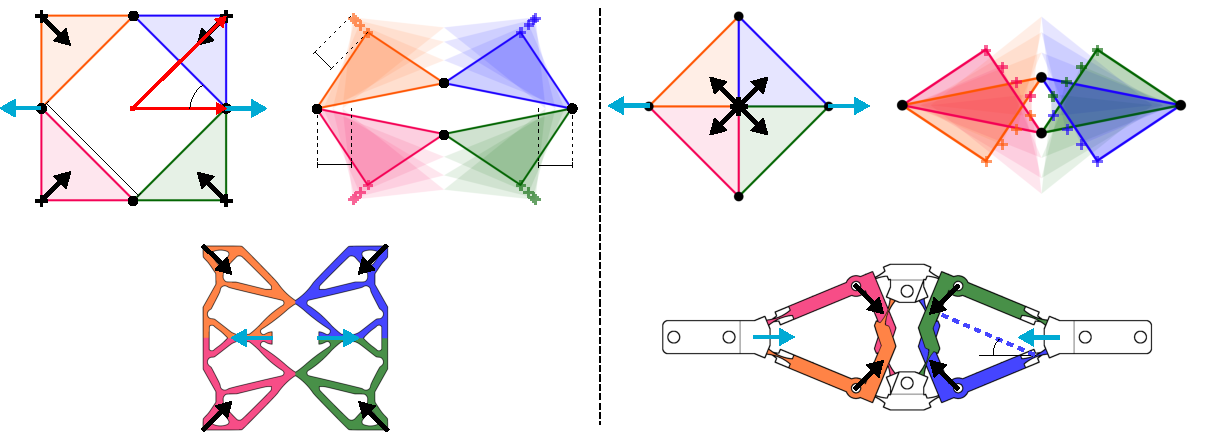
\includegraphics[width=\textwidth]{images/chap7/kinematic_schematics_models_reversed_legend_3.pdf}};
    \coordinate (ts0) at (\xLegendA,\yLegendTop); \node[align=left] at (ts0) {(a)};
    \coordinate (ts1) at (\xLegendB,\yLegendTop); \node[align=left] at (ts1) {(b)};
    \coordinate (ts2) at (\xLegendC,\yLegendTop); \node[align=left] at (ts2) {(c)};
    \coordinate (ts3) at (\xLegendD,\yLegendTop); \node[align=left] at (ts3) {(d)};
    \coordinate (ts4) at (\xLegendE,\yLegendBottom); \node[align=left] at (ts4) {(e)};
    \coordinate (ts5) at (\xLegendF,\yLegendBottom); \node[align=left] at (ts5) {(f)};

    %%%%%%%%%%%%%%%%%%%%%%%%%%%%%%%%%%%%%
    \node[align=left] at (\xLegendA+0.6,\yLegendTop+1.7) {$\theta$};
% 		\node[align=left] at (\xLegendA+0.45,\yLegendTop+2.1) {$\theta$};
% 		\node[align=left] at (\xLegendA+1.8,\yLegendTop+1.) {$L_s$};
    \node[align=left] at (\xLegendA+0.55,\yLegendTop+1.18) {\color{red}$\frac{x}{2}$};
    \node[align=left,rotate=45] at (\xLegendA+0.25,\yLegendTop+2.0) {\small\color{red}$R$};
    \node[align=left,rotate=-44] at (\xLegendA-0.2,\yLegendTop+1.0) {$L_h$};

    \node[align=left] at (\xLegendB+1.3,\yLegendTop+0.4) {$\frac{\Delta x}{2}$};
    \node[align=left] at (\xLegendB-1.5,\yLegendTop+0.4) {$\frac{\Delta x}{2}$};
% 		\node[align=left,rotate=-45] at (\xLegendB-2.1,\yLegendTop+2.35) {\small$R(\Delta x)$};
    \node[align=left,rotate=-45] at (\xLegendB-1.8,\yLegendTop+1.85) {\small$\Delta R$};

    \node[align=left] at (\xLegendF+0.55,\yLegendBottom+1.35) {$\theta_0$};
    % \draw[help lines] (0,0) grid (16,4); % $$$$$$$$$$$$$ HELPS A LOT FOR COORDINATES $$$$$$$
\end{tikzpicture}
\end{document}
}
  \caption{Kinematic diagram of proposed design where the black dots represent ideal pivots, the blue and black arrows represent the input and output displacement, respectively. On the left: the outward-triangle configuration with a) the initial position and b) the displaced one. On the right-hand side: the inward-triangle configuration achieving a stroke amplification with c) the initial position and d) the displaced one. e) represents mandrel topology generated with 2D topology optimization which behaves similarly to the outward version. f) shows the 2.5D adaptation of the inward version into a flexure-based mechanism distributed over multiple layers, and with a reversed actuation direction.}
  \label{fig:mandrel-kinematic}
\end{figure}

When examining the concept behind the mandrel mechanism, the conclusion can be made that the driving structure consists of four right-angled isosceles triangles which represent the four claws of the mandrel. Furthermore, the pivots, being constrained along the horizontal and vertical axes due to symmetry, force the outputs to move along a $45^{\circ}$ path. However, upon careful examination, these constraints can be satisfied in two distinct configurations as shown in \cref{fig:mandrel-kinematic}(a) and (c). The four triangles can be position inwardly or outwardly. Due to the inward-facing configuration having overlapping triangles, this topology cannot be generated from a 2D design space. The main advantage of the inward-facing configuration compared to the outward-facing configuration is the stroke amplification of the output vertices based on the stroke of the SMA coil contraction. It is also important to note that the direction of the radial output depends on the direction of the input displacement. Thus, the gripper can be made to open or close when the SMA coil is heated. By attaching the SMA coil to the vertical pivots rather than the horizontal ones, the gripper can be made to be always opened or always closed.

\subsubsection{Determining the Relationship between the Hinges and the SMA Stroke}
The stroke amplification, $\gamma$, of the system is not uniform and is dependant on the position of the mechanism, $x$. This amplification factor can be described by deriving the output vertex position, $R$, with respect to the input vertex position, $x$, and can be expressed analytically as :
\begin{equation}
\gamma(x) = \frac{\partial R(x)}{\partial x} = \frac{1}{2\sqrt{2}}\left(1-\text{sign}(\alpha)\frac{x}{\sqrt{L_{h}^2-\left(\frac{x}{2}\right)^2}} \right)
\label{eq:1}
\end{equation}
where,
\begin{equation}
\begin{split}
    R(x) &= L_{h}\cos\left(\theta(x) - \alpha\right)\\
     &= \frac{1}{\sqrt{2}} \left(\frac{x}{2} +\text{sign}(\alpha) \sqrt{L_{h}^2-\left(\frac{x}{2}\right)^2}\right),
    \label{eq:7}
\end{split}
\end{equation}
with,
\begin{equation}
\theta(x) = \arccos{\left(\frac{x}{2L_{h}}\right)} \quad \text{and} \quad \alpha=\pm\frac{\pi}{4}.
\label{eq:theta}
\end{equation}
Here, $L_h$ represents the length of the hypotenuse of each triangle, $\theta$ represents the angle between the horizontal and the hypotenuse, $\alpha$ represents the angle between the hypotenuse and the side of the triangle and can equal a value of $\pm\frac{\pi}{4}$. This angle is defined as positive for the outward-facing configuration and as negative for the inward-facing one. Here, the output stroke is majorly dependant on the sign of the angle $\alpha$. The outward configuration has a stroke amplification of less than one for almost all possible inputs, implying a stroke reduction. While, on the other hand, the inward configuration has a stroke amplification large than one. In the context of a gripper, the inward version was chosen for its larger output stroke.

\subsubsection{Simple Kinematics to a Compliant Mechanism}
The kinematic schematic is composed of only simple hinges and rigid links. This makes it the ideal candidate for implementation using flexure-based hinges. In this case, as shown in \cref{fig:mech_stages}, truncated semi-circular flexure hinges were selected for their ability to avoid high localised stress concentration and allow for an acceptable angular stroke as displayed in the work by \todocite.

\begin{figure}[t] % t for top of the page, H could be put to impose the position of the float
  \centering
  \resizebox{\textwidth}{!}{% !TEX root = ../sethomas_thesis_main.tex
\documentclass[border=1mm,
               class=article
               preview]{standalone}
\usepackage{tikz}
\begin{document}
\begin{tikzpicture}
    \pgfmathsetmacro{\YDelta}{1.1};%Offset for adding the side view

    \pgfmathsetmacro{\xLegendTop}{0.2};
    \pgfmathsetmacro{\yLegendTop}{5.3+\YDelta};

    \pgfmathsetmacro{\xLegendBottom}{1.1}; \pgfmathsetmacro{\yLegendBottom}{2.6+\YDelta};

    \pgfmathsetmacro{\xLegendSide}{0.2}; \pgfmathsetmacro{\yLegendSide}{0.65}

    % \node[anchor=south west,inner sep=0] (graph) at (0,0){\includegraphics[width=0.4\textwidth]{img/mechanism_iso_axes.png}};
    \node[anchor=south west,inner sep=0] (graph) at (0,0){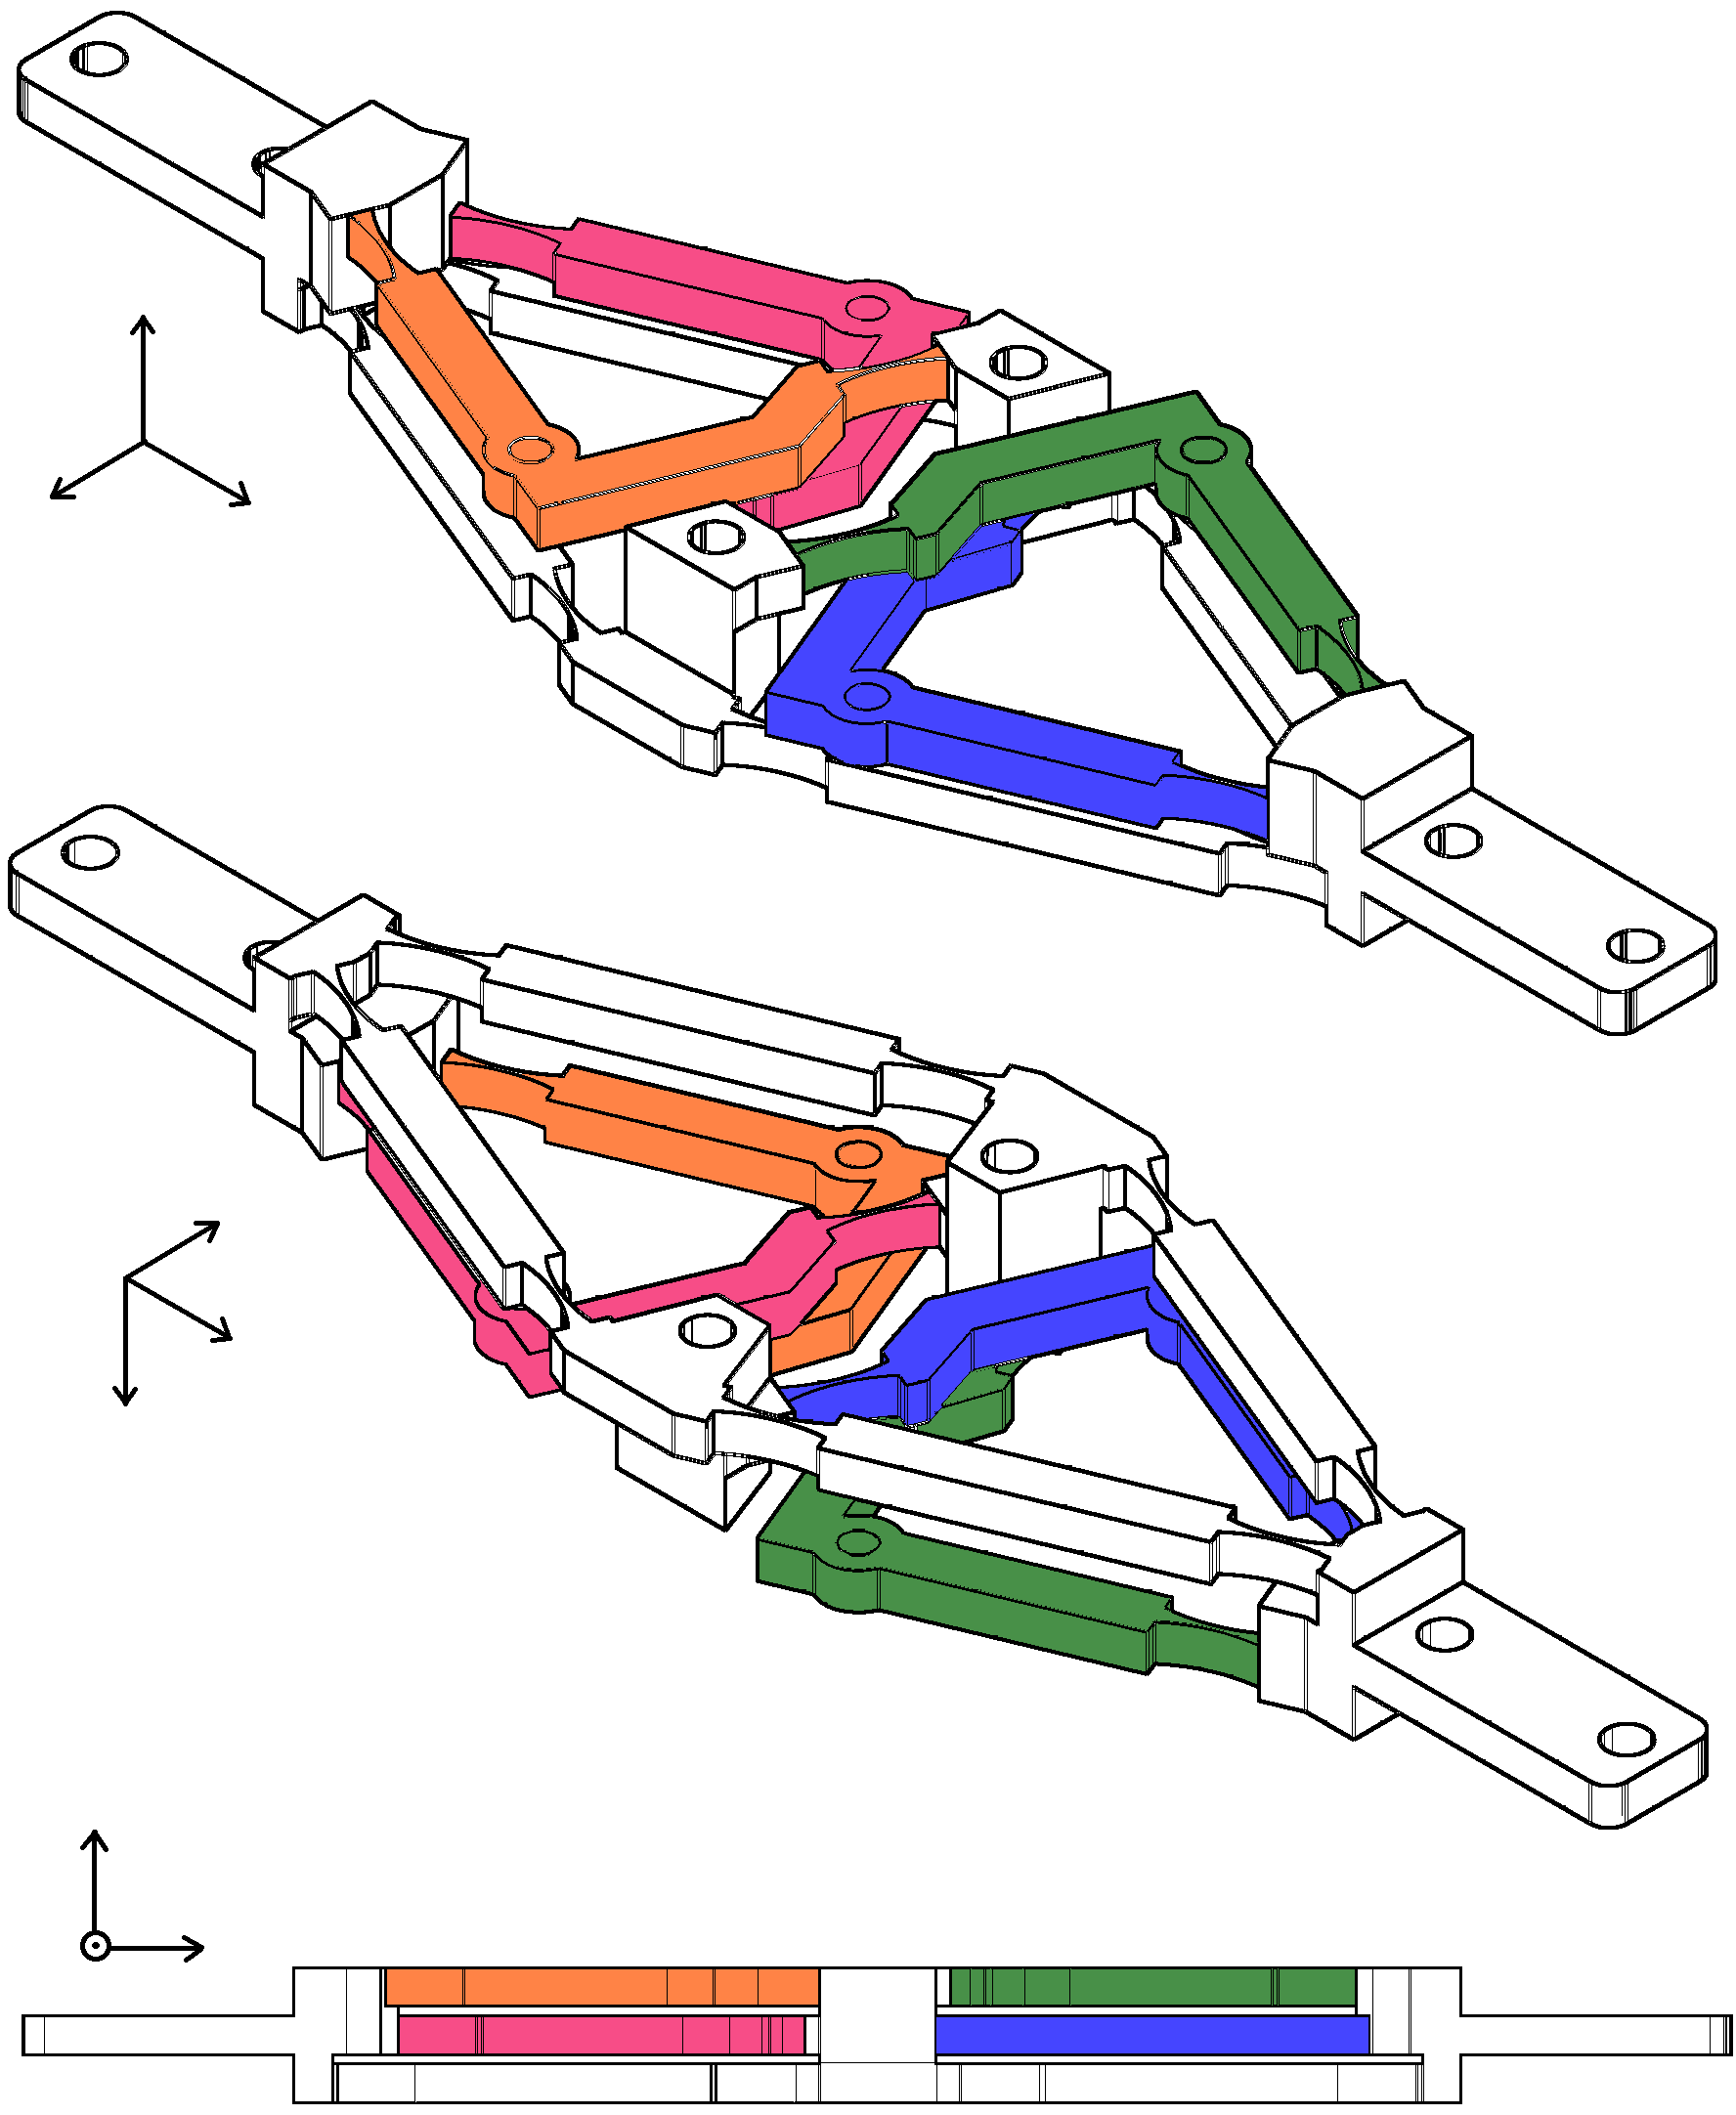
\includegraphics[width=0.4\textwidth]{images/chap7/mechanism_iso_axes_side.png}};
    \begin{scope}[x={(graph.south east)},y={(graph.north west)}]
        \node[align=left] at (0.04,0.742) {\footnotesize x};
        \node[align=left] at (0.15,0.735) {\footnotesize y};
        \node[align=left] at (0.06,0.85) {\footnotesize z};

        \node[align=left] at (0.095,0.445) {\footnotesize x};
        \node[align=left] at (0.155,0.345) {\footnotesize y};
        \node[align=left] at (0.045,0.34) {\footnotesize z};

        \node[align=left] at (0.03,0.1) {\footnotesize x};
        \node[align=left] at (0.135,0.1) {\footnotesize y};
        \node[align=left] at (0.08,0.155) {\footnotesize z};
    \end{scope}

    \pgfmathsetmacro{\xStartLine}{\xLegendSide-0.2};
    \pgfmathsetmacro{\xStopLine}{\xLegendSide+7};
    \draw[densely dotted] (\xStartLine,\yLegendSide-0.17) -- (\xStopLine,\yLegendSide-0.17);
    \node[align=left] at (\xStopLine+0.3,\yLegendSide-0.14) {\small $L_1$};
    \draw[densely dotted] (\xStartLine,\yLegendSide-0.37) -- (\xStopLine,\yLegendSide-0.37);
    \node[align=right] at (\xStartLine-0.3,\yLegendSide-0.34) {\small $L_2$}; %,draw,circle,inner sep=0.1pt
    \draw[densely dotted] (\xStartLine,\yLegendSide-0.57) -- (\xStopLine,\yLegendSide-0.57);
    \node[align=left] at (\xStopLine+0.3,\yLegendSide-0.6) {\small $L_3$};

    \pgfmathsetmacro{\xZOOM}{7.4};
    \pgfmathsetmacro{\yZOOM}{7.2};
    \node[anchor=north east,inner sep=0] (graph) at (\xZOOM,\yZOOM){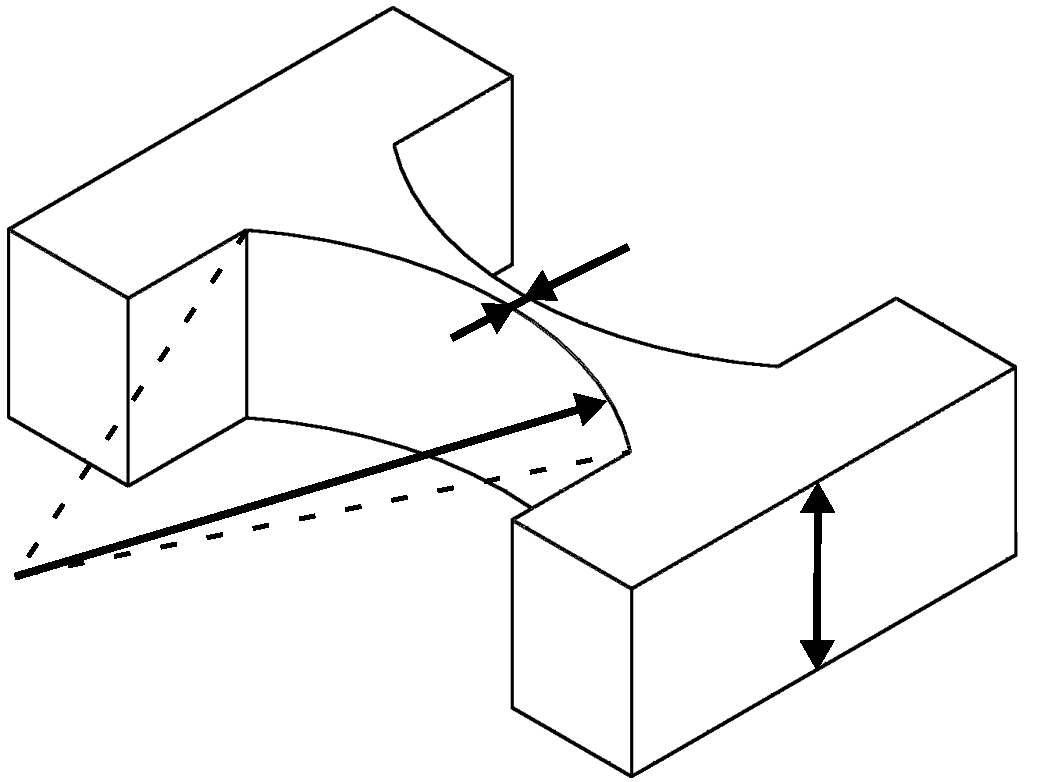
\includegraphics[width=2.5cm]{images/chap7/pivot.pdf}};
    \node[align=left] at (\xZOOM-1.,\yZOOM-0.45) {$e$};
    \node[align=left] at (\xZOOM-0.4,\yZOOM-1.3) {$b$};
    \node[align=left] at (\xZOOM-1.7,\yZOOM-1) {$r$};
    % \draw[help lines] (0,0) grid (8,8); % $$$$$$$$$$$$$ HELPS A LOT FOR COORDINATES $$$$$$$
\end{tikzpicture}
\end{document}
}
  \caption{Different views of the flexure-based compliant mechanism spreading over multiple stages, and parametrized flexure pivot.}
  \label{fig:mech_stages}
\end{figure}

As stated earlier, the inward-facing triangle configuration was chosen and due to fact that the triangles overlap during actuation, it makes it impossible to be implemented in a 2D design space. Thus, as shown in \cref{fig:mech_stages}, a 2.D design approach was implemented where each overlapping triangle is stacked in the 3\textsuperscript{rd} dimension. The mechanism is distributed among different superimposed layers linked at the vertices of the triangle to replicated the kinematic schematic. This adaptation to 2.5D design does not impact the functionality of the mechanism as long as the hinges are considered infinitely rigid when bending in any other direction other than the desired one. Here, two layers are implemented to accommodate the four triangles : the $L_1$ stage comprising of the green and orange triangles, and the $L_2$ stage comprising of the pink and blue triangles.

In the case of the ideal kinematic schematic, the triangles are attached at a single point to form a parallelogram. However, this is difficult to implement with a flexure-based solution due to the rigid links having a non-null width. This adds unwanted links and hinges to the kinematic chain which results in undesired Degrees of Freedom (DoF). This parasitic DoF is overcome by adding a third DoF-inhibiting stage, $L_3$, to the 2.5D design as shown in \cref{fig:mech_stages}.

As the goal of this gripper is for drone delivery purposes, another stage, which behaves as the frame of the drone, can be added to the design. For mechanism to behave as intended in the kinematic schematic, the left and right input vertices must be constraint to move along a single line. In this case, for simplicity, this constraint has been implemented using a rail. For a future drone mounted setup, an additional stage can be added to perform this required constraint, showing the advantage of the 2.5D design approach.

\subsubsection{Sizing of the Biasing Compliant Mechanism}
Based on the proposed design methodology, the goal of the mechanism is to create a kinematic stage that also behaves as the passive biasing element for the SMA coil. The inherent stiffness of the overall compliant mechanism due to the flexural hinges is harness to prestretch the SMA for activation. Thus, in order to size the actuator and the corresponding biasing element, an analytical model of the stiffness must be developed. Using the pseudo-rigid model, as presented in the work by \cite{heneinConceptionStructuresArticulees2005}, the flexural hinges can be considered as torsional spring with a constant angular stiffness, $K_\theta$. As detailed in \cref{chap:design-methodology}, the stiffness of the compliant structure requires an expression for the relationship between angular position of the flexural hinge and the contraction of the SMA, $\theta(\Delta x)$. In this case, this relationship can be expressed as :
\begin{equation}\label{eq:mandrel-theta-model}
\theta(\Delta x) = \arccos{\left(\frac{\Delta x}{2L_{h}} + \cos(\theta_0)\right)},
\end{equation}
with $\theta_0$ being the resting angle at which the mechanism is printer/fabricated as shown in \cref{fig:mandrel-kinematic}(f).

As detailed in the methodology, the next step is to calculate the potential energy within the system during deformation. Due to the symmetry of the mechanism, all the hinges store the same potential energy. Here, the $L_3$ stage has 8 hinges while the stages $L_1$ and $L_2$ have 4 hinges each. Thus, the total potential energy of the whole mechanism is :
\begin{equation}\label{eq:mandrel-potential-energy-model}
U_\mathrm{tot}(\Delta x) = 16\cdot U(\Delta x)
\end{equation}
The force-displacement characteristic of the mechanism is then given by :
\begin{equation}\label{eq:mandrel-force-model}
\begin{split}
    F(\Delta x) &= \lVert -\nabla{U_\text{tot}(\Delta x)}\rVert = \frac{\partial U_\text{tot}(\Delta x)}{\partial \Delta x}\\
     &= \frac{8K_{\theta}}{L_{h}}  \frac{(\theta(\Delta x)-\theta_{0})}{\sin(\theta(\Delta x))}.
\end{split}
\end{equation}
The resulting characteristic is plotted as shown in \cref{fig:mandrel-am-expt-compare}. Furthermore, the model is validated using experimental results obtained using a pull-tester. As the experimental results follow the model quite closely, it validates the working hypothesis and approximations used during the definition of the analytical model.
\begin{figure}[hbt!] % t for top of the page, H could be put to impose the position of the float
  \centering
  \resizebox{0.7\textwidth}{!}{%% Creator: Matplotlib, PGF backend
%%
%% To include the figure in your LaTeX document, write
%%   \input{<filename>.pgf}
%%
%% Make sure the required packages are loaded in your preamble
%%   \usepackage{pgf}
%%
%% and, on pdftex
%%   \usepackage[utf8]{inputenc}\DeclareUnicodeCharacter{2212}{-}
%%
%% or, on luatex and xetex
%%   \usepackage{unicode-math}
%%
%% Figures using additional raster images can only be included by \input if
%% they are in the same directory as the main LaTeX file. For loading figures
%% from other directories you can use the `import` package
%%   \usepackage{import}
%%
%% and then include the figures with
%%   \import{<path to file>}{<filename>.pgf}
%%
%% Matplotlib used the following preamble
%%
\begingroup%
\makeatletter%
\begin{pgfpicture}%
\pgfpathrectangle{\pgfpointorigin}{\pgfqpoint{6.300000in}{4.700000in}}%
\pgfusepath{use as bounding box, clip}%
\begin{pgfscope}%
\pgfsetbuttcap%
\pgfsetmiterjoin%
\pgfsetlinewidth{0.000000pt}%
\definecolor{currentstroke}{rgb}{0.000000,0.000000,0.000000}%
\pgfsetstrokecolor{currentstroke}%
\pgfsetstrokeopacity{0.000000}%
\pgfsetdash{}{0pt}%
\pgfpathmoveto{\pgfqpoint{-0.000000in}{-0.000000in}}%
\pgfpathlineto{\pgfqpoint{6.300000in}{-0.000000in}}%
\pgfpathlineto{\pgfqpoint{6.300000in}{4.700000in}}%
\pgfpathlineto{\pgfqpoint{-0.000000in}{4.700000in}}%
\pgfpathclose%
\pgfusepath{}%
\end{pgfscope}%
\begin{pgfscope}%
\pgfsetbuttcap%
\pgfsetmiterjoin%
\pgfsetlinewidth{0.000000pt}%
\definecolor{currentstroke}{rgb}{0.000000,0.000000,0.000000}%
\pgfsetstrokecolor{currentstroke}%
\pgfsetstrokeopacity{0.000000}%
\pgfsetdash{}{0pt}%
\pgfpathmoveto{\pgfqpoint{0.898145in}{0.670138in}}%
\pgfpathlineto{\pgfqpoint{6.200000in}{0.670138in}}%
\pgfpathlineto{\pgfqpoint{6.200000in}{4.600000in}}%
\pgfpathlineto{\pgfqpoint{0.898145in}{4.600000in}}%
\pgfpathclose%
\pgfusepath{}%
\end{pgfscope}%
\begin{pgfscope}%
\pgfpathrectangle{\pgfqpoint{0.898145in}{0.670138in}}{\pgfqpoint{5.301855in}{3.929862in}}%
\pgfusepath{clip}%
\pgfsetrectcap%
\pgfsetroundjoin%
\pgfsetlinewidth{0.803000pt}%
\definecolor{currentstroke}{rgb}{0.690196,0.690196,0.690196}%
\pgfsetstrokecolor{currentstroke}%
\pgfsetstrokeopacity{0.200000}%
\pgfsetdash{}{0pt}%
\pgfpathmoveto{\pgfqpoint{1.139138in}{0.670138in}}%
\pgfpathlineto{\pgfqpoint{1.139138in}{4.600000in}}%
\pgfusepath{stroke}%
\end{pgfscope}%
\begin{pgfscope}%
\pgfsetbuttcap%
\pgfsetroundjoin%
\definecolor{currentfill}{rgb}{0.000000,0.000000,0.000000}%
\pgfsetfillcolor{currentfill}%
\pgfsetlinewidth{0.803000pt}%
\definecolor{currentstroke}{rgb}{0.000000,0.000000,0.000000}%
\pgfsetstrokecolor{currentstroke}%
\pgfsetdash{}{0pt}%
\pgfsys@defobject{currentmarker}{\pgfqpoint{0.000000in}{-0.048611in}}{\pgfqpoint{0.000000in}{0.000000in}}{%
\pgfpathmoveto{\pgfqpoint{0.000000in}{0.000000in}}%
\pgfpathlineto{\pgfqpoint{0.000000in}{-0.048611in}}%
\pgfusepath{stroke,fill}%
}%
\begin{pgfscope}%
\pgfsys@transformshift{1.139138in}{0.670138in}%
\pgfsys@useobject{currentmarker}{}%
\end{pgfscope}%
\end{pgfscope}%
\begin{pgfscope}%
\definecolor{textcolor}{rgb}{0.000000,0.000000,0.000000}%
\pgfsetstrokecolor{textcolor}%
\pgfsetfillcolor{textcolor}%
\pgftext[x=1.139138in,y=0.572916in,,top]{\color{textcolor}\rmfamily\fontsize{14.000000}{16.800000}\selectfont \(\displaystyle {-6}\)}%
\end{pgfscope}%
\begin{pgfscope}%
\pgfpathrectangle{\pgfqpoint{0.898145in}{0.670138in}}{\pgfqpoint{5.301855in}{3.929862in}}%
\pgfusepath{clip}%
\pgfsetrectcap%
\pgfsetroundjoin%
\pgfsetlinewidth{0.803000pt}%
\definecolor{currentstroke}{rgb}{0.690196,0.690196,0.690196}%
\pgfsetstrokecolor{currentstroke}%
\pgfsetstrokeopacity{0.200000}%
\pgfsetdash{}{0pt}%
\pgfpathmoveto{\pgfqpoint{1.621125in}{0.670138in}}%
\pgfpathlineto{\pgfqpoint{1.621125in}{4.600000in}}%
\pgfusepath{stroke}%
\end{pgfscope}%
\begin{pgfscope}%
\pgfsetbuttcap%
\pgfsetroundjoin%
\definecolor{currentfill}{rgb}{0.000000,0.000000,0.000000}%
\pgfsetfillcolor{currentfill}%
\pgfsetlinewidth{0.803000pt}%
\definecolor{currentstroke}{rgb}{0.000000,0.000000,0.000000}%
\pgfsetstrokecolor{currentstroke}%
\pgfsetdash{}{0pt}%
\pgfsys@defobject{currentmarker}{\pgfqpoint{0.000000in}{-0.048611in}}{\pgfqpoint{0.000000in}{0.000000in}}{%
\pgfpathmoveto{\pgfqpoint{0.000000in}{0.000000in}}%
\pgfpathlineto{\pgfqpoint{0.000000in}{-0.048611in}}%
\pgfusepath{stroke,fill}%
}%
\begin{pgfscope}%
\pgfsys@transformshift{1.621125in}{0.670138in}%
\pgfsys@useobject{currentmarker}{}%
\end{pgfscope}%
\end{pgfscope}%
\begin{pgfscope}%
\definecolor{textcolor}{rgb}{0.000000,0.000000,0.000000}%
\pgfsetstrokecolor{textcolor}%
\pgfsetfillcolor{textcolor}%
\pgftext[x=1.621125in,y=0.572916in,,top]{\color{textcolor}\rmfamily\fontsize{14.000000}{16.800000}\selectfont \(\displaystyle {-5}\)}%
\end{pgfscope}%
\begin{pgfscope}%
\pgfpathrectangle{\pgfqpoint{0.898145in}{0.670138in}}{\pgfqpoint{5.301855in}{3.929862in}}%
\pgfusepath{clip}%
\pgfsetrectcap%
\pgfsetroundjoin%
\pgfsetlinewidth{0.803000pt}%
\definecolor{currentstroke}{rgb}{0.690196,0.690196,0.690196}%
\pgfsetstrokecolor{currentstroke}%
\pgfsetstrokeopacity{0.200000}%
\pgfsetdash{}{0pt}%
\pgfpathmoveto{\pgfqpoint{2.103112in}{0.670138in}}%
\pgfpathlineto{\pgfqpoint{2.103112in}{4.600000in}}%
\pgfusepath{stroke}%
\end{pgfscope}%
\begin{pgfscope}%
\pgfsetbuttcap%
\pgfsetroundjoin%
\definecolor{currentfill}{rgb}{0.000000,0.000000,0.000000}%
\pgfsetfillcolor{currentfill}%
\pgfsetlinewidth{0.803000pt}%
\definecolor{currentstroke}{rgb}{0.000000,0.000000,0.000000}%
\pgfsetstrokecolor{currentstroke}%
\pgfsetdash{}{0pt}%
\pgfsys@defobject{currentmarker}{\pgfqpoint{0.000000in}{-0.048611in}}{\pgfqpoint{0.000000in}{0.000000in}}{%
\pgfpathmoveto{\pgfqpoint{0.000000in}{0.000000in}}%
\pgfpathlineto{\pgfqpoint{0.000000in}{-0.048611in}}%
\pgfusepath{stroke,fill}%
}%
\begin{pgfscope}%
\pgfsys@transformshift{2.103112in}{0.670138in}%
\pgfsys@useobject{currentmarker}{}%
\end{pgfscope}%
\end{pgfscope}%
\begin{pgfscope}%
\definecolor{textcolor}{rgb}{0.000000,0.000000,0.000000}%
\pgfsetstrokecolor{textcolor}%
\pgfsetfillcolor{textcolor}%
\pgftext[x=2.103112in,y=0.572916in,,top]{\color{textcolor}\rmfamily\fontsize{14.000000}{16.800000}\selectfont \(\displaystyle {-4}\)}%
\end{pgfscope}%
\begin{pgfscope}%
\pgfpathrectangle{\pgfqpoint{0.898145in}{0.670138in}}{\pgfqpoint{5.301855in}{3.929862in}}%
\pgfusepath{clip}%
\pgfsetrectcap%
\pgfsetroundjoin%
\pgfsetlinewidth{0.803000pt}%
\definecolor{currentstroke}{rgb}{0.690196,0.690196,0.690196}%
\pgfsetstrokecolor{currentstroke}%
\pgfsetstrokeopacity{0.200000}%
\pgfsetdash{}{0pt}%
\pgfpathmoveto{\pgfqpoint{2.585099in}{0.670138in}}%
\pgfpathlineto{\pgfqpoint{2.585099in}{4.600000in}}%
\pgfusepath{stroke}%
\end{pgfscope}%
\begin{pgfscope}%
\pgfsetbuttcap%
\pgfsetroundjoin%
\definecolor{currentfill}{rgb}{0.000000,0.000000,0.000000}%
\pgfsetfillcolor{currentfill}%
\pgfsetlinewidth{0.803000pt}%
\definecolor{currentstroke}{rgb}{0.000000,0.000000,0.000000}%
\pgfsetstrokecolor{currentstroke}%
\pgfsetdash{}{0pt}%
\pgfsys@defobject{currentmarker}{\pgfqpoint{0.000000in}{-0.048611in}}{\pgfqpoint{0.000000in}{0.000000in}}{%
\pgfpathmoveto{\pgfqpoint{0.000000in}{0.000000in}}%
\pgfpathlineto{\pgfqpoint{0.000000in}{-0.048611in}}%
\pgfusepath{stroke,fill}%
}%
\begin{pgfscope}%
\pgfsys@transformshift{2.585099in}{0.670138in}%
\pgfsys@useobject{currentmarker}{}%
\end{pgfscope}%
\end{pgfscope}%
\begin{pgfscope}%
\definecolor{textcolor}{rgb}{0.000000,0.000000,0.000000}%
\pgfsetstrokecolor{textcolor}%
\pgfsetfillcolor{textcolor}%
\pgftext[x=2.585099in,y=0.572916in,,top]{\color{textcolor}\rmfamily\fontsize{14.000000}{16.800000}\selectfont \(\displaystyle {-3}\)}%
\end{pgfscope}%
\begin{pgfscope}%
\pgfpathrectangle{\pgfqpoint{0.898145in}{0.670138in}}{\pgfqpoint{5.301855in}{3.929862in}}%
\pgfusepath{clip}%
\pgfsetrectcap%
\pgfsetroundjoin%
\pgfsetlinewidth{0.803000pt}%
\definecolor{currentstroke}{rgb}{0.690196,0.690196,0.690196}%
\pgfsetstrokecolor{currentstroke}%
\pgfsetstrokeopacity{0.200000}%
\pgfsetdash{}{0pt}%
\pgfpathmoveto{\pgfqpoint{3.067086in}{0.670138in}}%
\pgfpathlineto{\pgfqpoint{3.067086in}{4.600000in}}%
\pgfusepath{stroke}%
\end{pgfscope}%
\begin{pgfscope}%
\pgfsetbuttcap%
\pgfsetroundjoin%
\definecolor{currentfill}{rgb}{0.000000,0.000000,0.000000}%
\pgfsetfillcolor{currentfill}%
\pgfsetlinewidth{0.803000pt}%
\definecolor{currentstroke}{rgb}{0.000000,0.000000,0.000000}%
\pgfsetstrokecolor{currentstroke}%
\pgfsetdash{}{0pt}%
\pgfsys@defobject{currentmarker}{\pgfqpoint{0.000000in}{-0.048611in}}{\pgfqpoint{0.000000in}{0.000000in}}{%
\pgfpathmoveto{\pgfqpoint{0.000000in}{0.000000in}}%
\pgfpathlineto{\pgfqpoint{0.000000in}{-0.048611in}}%
\pgfusepath{stroke,fill}%
}%
\begin{pgfscope}%
\pgfsys@transformshift{3.067086in}{0.670138in}%
\pgfsys@useobject{currentmarker}{}%
\end{pgfscope}%
\end{pgfscope}%
\begin{pgfscope}%
\definecolor{textcolor}{rgb}{0.000000,0.000000,0.000000}%
\pgfsetstrokecolor{textcolor}%
\pgfsetfillcolor{textcolor}%
\pgftext[x=3.067086in,y=0.572916in,,top]{\color{textcolor}\rmfamily\fontsize{14.000000}{16.800000}\selectfont \(\displaystyle {-2}\)}%
\end{pgfscope}%
\begin{pgfscope}%
\pgfpathrectangle{\pgfqpoint{0.898145in}{0.670138in}}{\pgfqpoint{5.301855in}{3.929862in}}%
\pgfusepath{clip}%
\pgfsetrectcap%
\pgfsetroundjoin%
\pgfsetlinewidth{0.803000pt}%
\definecolor{currentstroke}{rgb}{0.690196,0.690196,0.690196}%
\pgfsetstrokecolor{currentstroke}%
\pgfsetstrokeopacity{0.200000}%
\pgfsetdash{}{0pt}%
\pgfpathmoveto{\pgfqpoint{3.549072in}{0.670138in}}%
\pgfpathlineto{\pgfqpoint{3.549072in}{4.600000in}}%
\pgfusepath{stroke}%
\end{pgfscope}%
\begin{pgfscope}%
\pgfsetbuttcap%
\pgfsetroundjoin%
\definecolor{currentfill}{rgb}{0.000000,0.000000,0.000000}%
\pgfsetfillcolor{currentfill}%
\pgfsetlinewidth{0.803000pt}%
\definecolor{currentstroke}{rgb}{0.000000,0.000000,0.000000}%
\pgfsetstrokecolor{currentstroke}%
\pgfsetdash{}{0pt}%
\pgfsys@defobject{currentmarker}{\pgfqpoint{0.000000in}{-0.048611in}}{\pgfqpoint{0.000000in}{0.000000in}}{%
\pgfpathmoveto{\pgfqpoint{0.000000in}{0.000000in}}%
\pgfpathlineto{\pgfqpoint{0.000000in}{-0.048611in}}%
\pgfusepath{stroke,fill}%
}%
\begin{pgfscope}%
\pgfsys@transformshift{3.549072in}{0.670138in}%
\pgfsys@useobject{currentmarker}{}%
\end{pgfscope}%
\end{pgfscope}%
\begin{pgfscope}%
\definecolor{textcolor}{rgb}{0.000000,0.000000,0.000000}%
\pgfsetstrokecolor{textcolor}%
\pgfsetfillcolor{textcolor}%
\pgftext[x=3.549072in,y=0.572916in,,top]{\color{textcolor}\rmfamily\fontsize{14.000000}{16.800000}\selectfont \(\displaystyle {-1}\)}%
\end{pgfscope}%
\begin{pgfscope}%
\pgfpathrectangle{\pgfqpoint{0.898145in}{0.670138in}}{\pgfqpoint{5.301855in}{3.929862in}}%
\pgfusepath{clip}%
\pgfsetrectcap%
\pgfsetroundjoin%
\pgfsetlinewidth{0.803000pt}%
\definecolor{currentstroke}{rgb}{0.690196,0.690196,0.690196}%
\pgfsetstrokecolor{currentstroke}%
\pgfsetstrokeopacity{0.200000}%
\pgfsetdash{}{0pt}%
\pgfpathmoveto{\pgfqpoint{4.031059in}{0.670138in}}%
\pgfpathlineto{\pgfqpoint{4.031059in}{4.600000in}}%
\pgfusepath{stroke}%
\end{pgfscope}%
\begin{pgfscope}%
\pgfsetbuttcap%
\pgfsetroundjoin%
\definecolor{currentfill}{rgb}{0.000000,0.000000,0.000000}%
\pgfsetfillcolor{currentfill}%
\pgfsetlinewidth{0.803000pt}%
\definecolor{currentstroke}{rgb}{0.000000,0.000000,0.000000}%
\pgfsetstrokecolor{currentstroke}%
\pgfsetdash{}{0pt}%
\pgfsys@defobject{currentmarker}{\pgfqpoint{0.000000in}{-0.048611in}}{\pgfqpoint{0.000000in}{0.000000in}}{%
\pgfpathmoveto{\pgfqpoint{0.000000in}{0.000000in}}%
\pgfpathlineto{\pgfqpoint{0.000000in}{-0.048611in}}%
\pgfusepath{stroke,fill}%
}%
\begin{pgfscope}%
\pgfsys@transformshift{4.031059in}{0.670138in}%
\pgfsys@useobject{currentmarker}{}%
\end{pgfscope}%
\end{pgfscope}%
\begin{pgfscope}%
\definecolor{textcolor}{rgb}{0.000000,0.000000,0.000000}%
\pgfsetstrokecolor{textcolor}%
\pgfsetfillcolor{textcolor}%
\pgftext[x=4.031059in,y=0.572916in,,top]{\color{textcolor}\rmfamily\fontsize{14.000000}{16.800000}\selectfont \(\displaystyle {0}\)}%
\end{pgfscope}%
\begin{pgfscope}%
\pgfpathrectangle{\pgfqpoint{0.898145in}{0.670138in}}{\pgfqpoint{5.301855in}{3.929862in}}%
\pgfusepath{clip}%
\pgfsetrectcap%
\pgfsetroundjoin%
\pgfsetlinewidth{0.803000pt}%
\definecolor{currentstroke}{rgb}{0.690196,0.690196,0.690196}%
\pgfsetstrokecolor{currentstroke}%
\pgfsetstrokeopacity{0.200000}%
\pgfsetdash{}{0pt}%
\pgfpathmoveto{\pgfqpoint{4.513046in}{0.670138in}}%
\pgfpathlineto{\pgfqpoint{4.513046in}{4.600000in}}%
\pgfusepath{stroke}%
\end{pgfscope}%
\begin{pgfscope}%
\pgfsetbuttcap%
\pgfsetroundjoin%
\definecolor{currentfill}{rgb}{0.000000,0.000000,0.000000}%
\pgfsetfillcolor{currentfill}%
\pgfsetlinewidth{0.803000pt}%
\definecolor{currentstroke}{rgb}{0.000000,0.000000,0.000000}%
\pgfsetstrokecolor{currentstroke}%
\pgfsetdash{}{0pt}%
\pgfsys@defobject{currentmarker}{\pgfqpoint{0.000000in}{-0.048611in}}{\pgfqpoint{0.000000in}{0.000000in}}{%
\pgfpathmoveto{\pgfqpoint{0.000000in}{0.000000in}}%
\pgfpathlineto{\pgfqpoint{0.000000in}{-0.048611in}}%
\pgfusepath{stroke,fill}%
}%
\begin{pgfscope}%
\pgfsys@transformshift{4.513046in}{0.670138in}%
\pgfsys@useobject{currentmarker}{}%
\end{pgfscope}%
\end{pgfscope}%
\begin{pgfscope}%
\definecolor{textcolor}{rgb}{0.000000,0.000000,0.000000}%
\pgfsetstrokecolor{textcolor}%
\pgfsetfillcolor{textcolor}%
\pgftext[x=4.513046in,y=0.572916in,,top]{\color{textcolor}\rmfamily\fontsize{14.000000}{16.800000}\selectfont \(\displaystyle {1}\)}%
\end{pgfscope}%
\begin{pgfscope}%
\pgfpathrectangle{\pgfqpoint{0.898145in}{0.670138in}}{\pgfqpoint{5.301855in}{3.929862in}}%
\pgfusepath{clip}%
\pgfsetrectcap%
\pgfsetroundjoin%
\pgfsetlinewidth{0.803000pt}%
\definecolor{currentstroke}{rgb}{0.690196,0.690196,0.690196}%
\pgfsetstrokecolor{currentstroke}%
\pgfsetstrokeopacity{0.200000}%
\pgfsetdash{}{0pt}%
\pgfpathmoveto{\pgfqpoint{4.995033in}{0.670138in}}%
\pgfpathlineto{\pgfqpoint{4.995033in}{4.600000in}}%
\pgfusepath{stroke}%
\end{pgfscope}%
\begin{pgfscope}%
\pgfsetbuttcap%
\pgfsetroundjoin%
\definecolor{currentfill}{rgb}{0.000000,0.000000,0.000000}%
\pgfsetfillcolor{currentfill}%
\pgfsetlinewidth{0.803000pt}%
\definecolor{currentstroke}{rgb}{0.000000,0.000000,0.000000}%
\pgfsetstrokecolor{currentstroke}%
\pgfsetdash{}{0pt}%
\pgfsys@defobject{currentmarker}{\pgfqpoint{0.000000in}{-0.048611in}}{\pgfqpoint{0.000000in}{0.000000in}}{%
\pgfpathmoveto{\pgfqpoint{0.000000in}{0.000000in}}%
\pgfpathlineto{\pgfqpoint{0.000000in}{-0.048611in}}%
\pgfusepath{stroke,fill}%
}%
\begin{pgfscope}%
\pgfsys@transformshift{4.995033in}{0.670138in}%
\pgfsys@useobject{currentmarker}{}%
\end{pgfscope}%
\end{pgfscope}%
\begin{pgfscope}%
\definecolor{textcolor}{rgb}{0.000000,0.000000,0.000000}%
\pgfsetstrokecolor{textcolor}%
\pgfsetfillcolor{textcolor}%
\pgftext[x=4.995033in,y=0.572916in,,top]{\color{textcolor}\rmfamily\fontsize{14.000000}{16.800000}\selectfont \(\displaystyle {2}\)}%
\end{pgfscope}%
\begin{pgfscope}%
\pgfpathrectangle{\pgfqpoint{0.898145in}{0.670138in}}{\pgfqpoint{5.301855in}{3.929862in}}%
\pgfusepath{clip}%
\pgfsetrectcap%
\pgfsetroundjoin%
\pgfsetlinewidth{0.803000pt}%
\definecolor{currentstroke}{rgb}{0.690196,0.690196,0.690196}%
\pgfsetstrokecolor{currentstroke}%
\pgfsetstrokeopacity{0.200000}%
\pgfsetdash{}{0pt}%
\pgfpathmoveto{\pgfqpoint{5.477020in}{0.670138in}}%
\pgfpathlineto{\pgfqpoint{5.477020in}{4.600000in}}%
\pgfusepath{stroke}%
\end{pgfscope}%
\begin{pgfscope}%
\pgfsetbuttcap%
\pgfsetroundjoin%
\definecolor{currentfill}{rgb}{0.000000,0.000000,0.000000}%
\pgfsetfillcolor{currentfill}%
\pgfsetlinewidth{0.803000pt}%
\definecolor{currentstroke}{rgb}{0.000000,0.000000,0.000000}%
\pgfsetstrokecolor{currentstroke}%
\pgfsetdash{}{0pt}%
\pgfsys@defobject{currentmarker}{\pgfqpoint{0.000000in}{-0.048611in}}{\pgfqpoint{0.000000in}{0.000000in}}{%
\pgfpathmoveto{\pgfqpoint{0.000000in}{0.000000in}}%
\pgfpathlineto{\pgfqpoint{0.000000in}{-0.048611in}}%
\pgfusepath{stroke,fill}%
}%
\begin{pgfscope}%
\pgfsys@transformshift{5.477020in}{0.670138in}%
\pgfsys@useobject{currentmarker}{}%
\end{pgfscope}%
\end{pgfscope}%
\begin{pgfscope}%
\definecolor{textcolor}{rgb}{0.000000,0.000000,0.000000}%
\pgfsetstrokecolor{textcolor}%
\pgfsetfillcolor{textcolor}%
\pgftext[x=5.477020in,y=0.572916in,,top]{\color{textcolor}\rmfamily\fontsize{14.000000}{16.800000}\selectfont \(\displaystyle {3}\)}%
\end{pgfscope}%
\begin{pgfscope}%
\pgfpathrectangle{\pgfqpoint{0.898145in}{0.670138in}}{\pgfqpoint{5.301855in}{3.929862in}}%
\pgfusepath{clip}%
\pgfsetrectcap%
\pgfsetroundjoin%
\pgfsetlinewidth{0.803000pt}%
\definecolor{currentstroke}{rgb}{0.690196,0.690196,0.690196}%
\pgfsetstrokecolor{currentstroke}%
\pgfsetstrokeopacity{0.200000}%
\pgfsetdash{}{0pt}%
\pgfpathmoveto{\pgfqpoint{5.959007in}{0.670138in}}%
\pgfpathlineto{\pgfqpoint{5.959007in}{4.600000in}}%
\pgfusepath{stroke}%
\end{pgfscope}%
\begin{pgfscope}%
\pgfsetbuttcap%
\pgfsetroundjoin%
\definecolor{currentfill}{rgb}{0.000000,0.000000,0.000000}%
\pgfsetfillcolor{currentfill}%
\pgfsetlinewidth{0.803000pt}%
\definecolor{currentstroke}{rgb}{0.000000,0.000000,0.000000}%
\pgfsetstrokecolor{currentstroke}%
\pgfsetdash{}{0pt}%
\pgfsys@defobject{currentmarker}{\pgfqpoint{0.000000in}{-0.048611in}}{\pgfqpoint{0.000000in}{0.000000in}}{%
\pgfpathmoveto{\pgfqpoint{0.000000in}{0.000000in}}%
\pgfpathlineto{\pgfqpoint{0.000000in}{-0.048611in}}%
\pgfusepath{stroke,fill}%
}%
\begin{pgfscope}%
\pgfsys@transformshift{5.959007in}{0.670138in}%
\pgfsys@useobject{currentmarker}{}%
\end{pgfscope}%
\end{pgfscope}%
\begin{pgfscope}%
\definecolor{textcolor}{rgb}{0.000000,0.000000,0.000000}%
\pgfsetstrokecolor{textcolor}%
\pgfsetfillcolor{textcolor}%
\pgftext[x=5.959007in,y=0.572916in,,top]{\color{textcolor}\rmfamily\fontsize{14.000000}{16.800000}\selectfont \(\displaystyle {4}\)}%
\end{pgfscope}%
\begin{pgfscope}%
\definecolor{textcolor}{rgb}{0.000000,0.000000,0.000000}%
\pgfsetstrokecolor{textcolor}%
\pgfsetfillcolor{textcolor}%
\pgftext[x=3.549072in,y=0.339583in,,top]{\color{textcolor}\rmfamily\fontsize{16.000000}{19.200000}\selectfont Displacement [mm]}%
\end{pgfscope}%
\begin{pgfscope}%
\pgfpathrectangle{\pgfqpoint{0.898145in}{0.670138in}}{\pgfqpoint{5.301855in}{3.929862in}}%
\pgfusepath{clip}%
\pgfsetrectcap%
\pgfsetroundjoin%
\pgfsetlinewidth{0.803000pt}%
\definecolor{currentstroke}{rgb}{0.690196,0.690196,0.690196}%
\pgfsetstrokecolor{currentstroke}%
\pgfsetstrokeopacity{0.200000}%
\pgfsetdash{}{0pt}%
\pgfpathmoveto{\pgfqpoint{0.898145in}{0.763706in}}%
\pgfpathlineto{\pgfqpoint{6.200000in}{0.763706in}}%
\pgfusepath{stroke}%
\end{pgfscope}%
\begin{pgfscope}%
\pgfsetbuttcap%
\pgfsetroundjoin%
\definecolor{currentfill}{rgb}{0.000000,0.000000,0.000000}%
\pgfsetfillcolor{currentfill}%
\pgfsetlinewidth{0.803000pt}%
\definecolor{currentstroke}{rgb}{0.000000,0.000000,0.000000}%
\pgfsetstrokecolor{currentstroke}%
\pgfsetdash{}{0pt}%
\pgfsys@defobject{currentmarker}{\pgfqpoint{-0.048611in}{0.000000in}}{\pgfqpoint{-0.000000in}{0.000000in}}{%
\pgfpathmoveto{\pgfqpoint{-0.000000in}{0.000000in}}%
\pgfpathlineto{\pgfqpoint{-0.048611in}{0.000000in}}%
\pgfusepath{stroke,fill}%
}%
\begin{pgfscope}%
\pgfsys@transformshift{0.898145in}{0.763706in}%
\pgfsys@useobject{currentmarker}{}%
\end{pgfscope}%
\end{pgfscope}%
\begin{pgfscope}%
\definecolor{textcolor}{rgb}{0.000000,0.000000,0.000000}%
\pgfsetstrokecolor{textcolor}%
\pgfsetfillcolor{textcolor}%
\pgftext[x=0.395138in, y=0.694262in, left, base]{\color{textcolor}\rmfamily\fontsize{14.000000}{16.800000}\selectfont \(\displaystyle {-2.5}\)}%
\end{pgfscope}%
\begin{pgfscope}%
\pgfpathrectangle{\pgfqpoint{0.898145in}{0.670138in}}{\pgfqpoint{5.301855in}{3.929862in}}%
\pgfusepath{clip}%
\pgfsetrectcap%
\pgfsetroundjoin%
\pgfsetlinewidth{0.803000pt}%
\definecolor{currentstroke}{rgb}{0.690196,0.690196,0.690196}%
\pgfsetstrokecolor{currentstroke}%
\pgfsetstrokeopacity{0.200000}%
\pgfsetdash{}{0pt}%
\pgfpathmoveto{\pgfqpoint{0.898145in}{1.231547in}}%
\pgfpathlineto{\pgfqpoint{6.200000in}{1.231547in}}%
\pgfusepath{stroke}%
\end{pgfscope}%
\begin{pgfscope}%
\pgfsetbuttcap%
\pgfsetroundjoin%
\definecolor{currentfill}{rgb}{0.000000,0.000000,0.000000}%
\pgfsetfillcolor{currentfill}%
\pgfsetlinewidth{0.803000pt}%
\definecolor{currentstroke}{rgb}{0.000000,0.000000,0.000000}%
\pgfsetstrokecolor{currentstroke}%
\pgfsetdash{}{0pt}%
\pgfsys@defobject{currentmarker}{\pgfqpoint{-0.048611in}{0.000000in}}{\pgfqpoint{-0.000000in}{0.000000in}}{%
\pgfpathmoveto{\pgfqpoint{-0.000000in}{0.000000in}}%
\pgfpathlineto{\pgfqpoint{-0.048611in}{0.000000in}}%
\pgfusepath{stroke,fill}%
}%
\begin{pgfscope}%
\pgfsys@transformshift{0.898145in}{1.231547in}%
\pgfsys@useobject{currentmarker}{}%
\end{pgfscope}%
\end{pgfscope}%
\begin{pgfscope}%
\definecolor{textcolor}{rgb}{0.000000,0.000000,0.000000}%
\pgfsetstrokecolor{textcolor}%
\pgfsetfillcolor{textcolor}%
\pgftext[x=0.395138in, y=1.162103in, left, base]{\color{textcolor}\rmfamily\fontsize{14.000000}{16.800000}\selectfont \(\displaystyle {-2.0}\)}%
\end{pgfscope}%
\begin{pgfscope}%
\pgfpathrectangle{\pgfqpoint{0.898145in}{0.670138in}}{\pgfqpoint{5.301855in}{3.929862in}}%
\pgfusepath{clip}%
\pgfsetrectcap%
\pgfsetroundjoin%
\pgfsetlinewidth{0.803000pt}%
\definecolor{currentstroke}{rgb}{0.690196,0.690196,0.690196}%
\pgfsetstrokecolor{currentstroke}%
\pgfsetstrokeopacity{0.200000}%
\pgfsetdash{}{0pt}%
\pgfpathmoveto{\pgfqpoint{0.898145in}{1.699388in}}%
\pgfpathlineto{\pgfqpoint{6.200000in}{1.699388in}}%
\pgfusepath{stroke}%
\end{pgfscope}%
\begin{pgfscope}%
\pgfsetbuttcap%
\pgfsetroundjoin%
\definecolor{currentfill}{rgb}{0.000000,0.000000,0.000000}%
\pgfsetfillcolor{currentfill}%
\pgfsetlinewidth{0.803000pt}%
\definecolor{currentstroke}{rgb}{0.000000,0.000000,0.000000}%
\pgfsetstrokecolor{currentstroke}%
\pgfsetdash{}{0pt}%
\pgfsys@defobject{currentmarker}{\pgfqpoint{-0.048611in}{0.000000in}}{\pgfqpoint{-0.000000in}{0.000000in}}{%
\pgfpathmoveto{\pgfqpoint{-0.000000in}{0.000000in}}%
\pgfpathlineto{\pgfqpoint{-0.048611in}{0.000000in}}%
\pgfusepath{stroke,fill}%
}%
\begin{pgfscope}%
\pgfsys@transformshift{0.898145in}{1.699388in}%
\pgfsys@useobject{currentmarker}{}%
\end{pgfscope}%
\end{pgfscope}%
\begin{pgfscope}%
\definecolor{textcolor}{rgb}{0.000000,0.000000,0.000000}%
\pgfsetstrokecolor{textcolor}%
\pgfsetfillcolor{textcolor}%
\pgftext[x=0.395138in, y=1.629943in, left, base]{\color{textcolor}\rmfamily\fontsize{14.000000}{16.800000}\selectfont \(\displaystyle {-1.5}\)}%
\end{pgfscope}%
\begin{pgfscope}%
\pgfpathrectangle{\pgfqpoint{0.898145in}{0.670138in}}{\pgfqpoint{5.301855in}{3.929862in}}%
\pgfusepath{clip}%
\pgfsetrectcap%
\pgfsetroundjoin%
\pgfsetlinewidth{0.803000pt}%
\definecolor{currentstroke}{rgb}{0.690196,0.690196,0.690196}%
\pgfsetstrokecolor{currentstroke}%
\pgfsetstrokeopacity{0.200000}%
\pgfsetdash{}{0pt}%
\pgfpathmoveto{\pgfqpoint{0.898145in}{2.167228in}}%
\pgfpathlineto{\pgfqpoint{6.200000in}{2.167228in}}%
\pgfusepath{stroke}%
\end{pgfscope}%
\begin{pgfscope}%
\pgfsetbuttcap%
\pgfsetroundjoin%
\definecolor{currentfill}{rgb}{0.000000,0.000000,0.000000}%
\pgfsetfillcolor{currentfill}%
\pgfsetlinewidth{0.803000pt}%
\definecolor{currentstroke}{rgb}{0.000000,0.000000,0.000000}%
\pgfsetstrokecolor{currentstroke}%
\pgfsetdash{}{0pt}%
\pgfsys@defobject{currentmarker}{\pgfqpoint{-0.048611in}{0.000000in}}{\pgfqpoint{-0.000000in}{0.000000in}}{%
\pgfpathmoveto{\pgfqpoint{-0.000000in}{0.000000in}}%
\pgfpathlineto{\pgfqpoint{-0.048611in}{0.000000in}}%
\pgfusepath{stroke,fill}%
}%
\begin{pgfscope}%
\pgfsys@transformshift{0.898145in}{2.167228in}%
\pgfsys@useobject{currentmarker}{}%
\end{pgfscope}%
\end{pgfscope}%
\begin{pgfscope}%
\definecolor{textcolor}{rgb}{0.000000,0.000000,0.000000}%
\pgfsetstrokecolor{textcolor}%
\pgfsetfillcolor{textcolor}%
\pgftext[x=0.395138in, y=2.097784in, left, base]{\color{textcolor}\rmfamily\fontsize{14.000000}{16.800000}\selectfont \(\displaystyle {-1.0}\)}%
\end{pgfscope}%
\begin{pgfscope}%
\pgfpathrectangle{\pgfqpoint{0.898145in}{0.670138in}}{\pgfqpoint{5.301855in}{3.929862in}}%
\pgfusepath{clip}%
\pgfsetrectcap%
\pgfsetroundjoin%
\pgfsetlinewidth{0.803000pt}%
\definecolor{currentstroke}{rgb}{0.690196,0.690196,0.690196}%
\pgfsetstrokecolor{currentstroke}%
\pgfsetstrokeopacity{0.200000}%
\pgfsetdash{}{0pt}%
\pgfpathmoveto{\pgfqpoint{0.898145in}{2.635069in}}%
\pgfpathlineto{\pgfqpoint{6.200000in}{2.635069in}}%
\pgfusepath{stroke}%
\end{pgfscope}%
\begin{pgfscope}%
\pgfsetbuttcap%
\pgfsetroundjoin%
\definecolor{currentfill}{rgb}{0.000000,0.000000,0.000000}%
\pgfsetfillcolor{currentfill}%
\pgfsetlinewidth{0.803000pt}%
\definecolor{currentstroke}{rgb}{0.000000,0.000000,0.000000}%
\pgfsetstrokecolor{currentstroke}%
\pgfsetdash{}{0pt}%
\pgfsys@defobject{currentmarker}{\pgfqpoint{-0.048611in}{0.000000in}}{\pgfqpoint{-0.000000in}{0.000000in}}{%
\pgfpathmoveto{\pgfqpoint{-0.000000in}{0.000000in}}%
\pgfpathlineto{\pgfqpoint{-0.048611in}{0.000000in}}%
\pgfusepath{stroke,fill}%
}%
\begin{pgfscope}%
\pgfsys@transformshift{0.898145in}{2.635069in}%
\pgfsys@useobject{currentmarker}{}%
\end{pgfscope}%
\end{pgfscope}%
\begin{pgfscope}%
\definecolor{textcolor}{rgb}{0.000000,0.000000,0.000000}%
\pgfsetstrokecolor{textcolor}%
\pgfsetfillcolor{textcolor}%
\pgftext[x=0.395138in, y=2.565625in, left, base]{\color{textcolor}\rmfamily\fontsize{14.000000}{16.800000}\selectfont \(\displaystyle {-0.5}\)}%
\end{pgfscope}%
\begin{pgfscope}%
\pgfpathrectangle{\pgfqpoint{0.898145in}{0.670138in}}{\pgfqpoint{5.301855in}{3.929862in}}%
\pgfusepath{clip}%
\pgfsetrectcap%
\pgfsetroundjoin%
\pgfsetlinewidth{0.803000pt}%
\definecolor{currentstroke}{rgb}{0.690196,0.690196,0.690196}%
\pgfsetstrokecolor{currentstroke}%
\pgfsetstrokeopacity{0.200000}%
\pgfsetdash{}{0pt}%
\pgfpathmoveto{\pgfqpoint{0.898145in}{3.102910in}}%
\pgfpathlineto{\pgfqpoint{6.200000in}{3.102910in}}%
\pgfusepath{stroke}%
\end{pgfscope}%
\begin{pgfscope}%
\pgfsetbuttcap%
\pgfsetroundjoin%
\definecolor{currentfill}{rgb}{0.000000,0.000000,0.000000}%
\pgfsetfillcolor{currentfill}%
\pgfsetlinewidth{0.803000pt}%
\definecolor{currentstroke}{rgb}{0.000000,0.000000,0.000000}%
\pgfsetstrokecolor{currentstroke}%
\pgfsetdash{}{0pt}%
\pgfsys@defobject{currentmarker}{\pgfqpoint{-0.048611in}{0.000000in}}{\pgfqpoint{-0.000000in}{0.000000in}}{%
\pgfpathmoveto{\pgfqpoint{-0.000000in}{0.000000in}}%
\pgfpathlineto{\pgfqpoint{-0.048611in}{0.000000in}}%
\pgfusepath{stroke,fill}%
}%
\begin{pgfscope}%
\pgfsys@transformshift{0.898145in}{3.102910in}%
\pgfsys@useobject{currentmarker}{}%
\end{pgfscope}%
\end{pgfscope}%
\begin{pgfscope}%
\definecolor{textcolor}{rgb}{0.000000,0.000000,0.000000}%
\pgfsetstrokecolor{textcolor}%
\pgfsetfillcolor{textcolor}%
\pgftext[x=0.550694in, y=3.033465in, left, base]{\color{textcolor}\rmfamily\fontsize{14.000000}{16.800000}\selectfont \(\displaystyle {0.0}\)}%
\end{pgfscope}%
\begin{pgfscope}%
\pgfpathrectangle{\pgfqpoint{0.898145in}{0.670138in}}{\pgfqpoint{5.301855in}{3.929862in}}%
\pgfusepath{clip}%
\pgfsetrectcap%
\pgfsetroundjoin%
\pgfsetlinewidth{0.803000pt}%
\definecolor{currentstroke}{rgb}{0.690196,0.690196,0.690196}%
\pgfsetstrokecolor{currentstroke}%
\pgfsetstrokeopacity{0.200000}%
\pgfsetdash{}{0pt}%
\pgfpathmoveto{\pgfqpoint{0.898145in}{3.570750in}}%
\pgfpathlineto{\pgfqpoint{6.200000in}{3.570750in}}%
\pgfusepath{stroke}%
\end{pgfscope}%
\begin{pgfscope}%
\pgfsetbuttcap%
\pgfsetroundjoin%
\definecolor{currentfill}{rgb}{0.000000,0.000000,0.000000}%
\pgfsetfillcolor{currentfill}%
\pgfsetlinewidth{0.803000pt}%
\definecolor{currentstroke}{rgb}{0.000000,0.000000,0.000000}%
\pgfsetstrokecolor{currentstroke}%
\pgfsetdash{}{0pt}%
\pgfsys@defobject{currentmarker}{\pgfqpoint{-0.048611in}{0.000000in}}{\pgfqpoint{-0.000000in}{0.000000in}}{%
\pgfpathmoveto{\pgfqpoint{-0.000000in}{0.000000in}}%
\pgfpathlineto{\pgfqpoint{-0.048611in}{0.000000in}}%
\pgfusepath{stroke,fill}%
}%
\begin{pgfscope}%
\pgfsys@transformshift{0.898145in}{3.570750in}%
\pgfsys@useobject{currentmarker}{}%
\end{pgfscope}%
\end{pgfscope}%
\begin{pgfscope}%
\definecolor{textcolor}{rgb}{0.000000,0.000000,0.000000}%
\pgfsetstrokecolor{textcolor}%
\pgfsetfillcolor{textcolor}%
\pgftext[x=0.550694in, y=3.501306in, left, base]{\color{textcolor}\rmfamily\fontsize{14.000000}{16.800000}\selectfont \(\displaystyle {0.5}\)}%
\end{pgfscope}%
\begin{pgfscope}%
\pgfpathrectangle{\pgfqpoint{0.898145in}{0.670138in}}{\pgfqpoint{5.301855in}{3.929862in}}%
\pgfusepath{clip}%
\pgfsetrectcap%
\pgfsetroundjoin%
\pgfsetlinewidth{0.803000pt}%
\definecolor{currentstroke}{rgb}{0.690196,0.690196,0.690196}%
\pgfsetstrokecolor{currentstroke}%
\pgfsetstrokeopacity{0.200000}%
\pgfsetdash{}{0pt}%
\pgfpathmoveto{\pgfqpoint{0.898145in}{4.038591in}}%
\pgfpathlineto{\pgfqpoint{6.200000in}{4.038591in}}%
\pgfusepath{stroke}%
\end{pgfscope}%
\begin{pgfscope}%
\pgfsetbuttcap%
\pgfsetroundjoin%
\definecolor{currentfill}{rgb}{0.000000,0.000000,0.000000}%
\pgfsetfillcolor{currentfill}%
\pgfsetlinewidth{0.803000pt}%
\definecolor{currentstroke}{rgb}{0.000000,0.000000,0.000000}%
\pgfsetstrokecolor{currentstroke}%
\pgfsetdash{}{0pt}%
\pgfsys@defobject{currentmarker}{\pgfqpoint{-0.048611in}{0.000000in}}{\pgfqpoint{-0.000000in}{0.000000in}}{%
\pgfpathmoveto{\pgfqpoint{-0.000000in}{0.000000in}}%
\pgfpathlineto{\pgfqpoint{-0.048611in}{0.000000in}}%
\pgfusepath{stroke,fill}%
}%
\begin{pgfscope}%
\pgfsys@transformshift{0.898145in}{4.038591in}%
\pgfsys@useobject{currentmarker}{}%
\end{pgfscope}%
\end{pgfscope}%
\begin{pgfscope}%
\definecolor{textcolor}{rgb}{0.000000,0.000000,0.000000}%
\pgfsetstrokecolor{textcolor}%
\pgfsetfillcolor{textcolor}%
\pgftext[x=0.550694in, y=3.969147in, left, base]{\color{textcolor}\rmfamily\fontsize{14.000000}{16.800000}\selectfont \(\displaystyle {1.0}\)}%
\end{pgfscope}%
\begin{pgfscope}%
\pgfpathrectangle{\pgfqpoint{0.898145in}{0.670138in}}{\pgfqpoint{5.301855in}{3.929862in}}%
\pgfusepath{clip}%
\pgfsetrectcap%
\pgfsetroundjoin%
\pgfsetlinewidth{0.803000pt}%
\definecolor{currentstroke}{rgb}{0.690196,0.690196,0.690196}%
\pgfsetstrokecolor{currentstroke}%
\pgfsetstrokeopacity{0.200000}%
\pgfsetdash{}{0pt}%
\pgfpathmoveto{\pgfqpoint{0.898145in}{4.506432in}}%
\pgfpathlineto{\pgfqpoint{6.200000in}{4.506432in}}%
\pgfusepath{stroke}%
\end{pgfscope}%
\begin{pgfscope}%
\pgfsetbuttcap%
\pgfsetroundjoin%
\definecolor{currentfill}{rgb}{0.000000,0.000000,0.000000}%
\pgfsetfillcolor{currentfill}%
\pgfsetlinewidth{0.803000pt}%
\definecolor{currentstroke}{rgb}{0.000000,0.000000,0.000000}%
\pgfsetstrokecolor{currentstroke}%
\pgfsetdash{}{0pt}%
\pgfsys@defobject{currentmarker}{\pgfqpoint{-0.048611in}{0.000000in}}{\pgfqpoint{-0.000000in}{0.000000in}}{%
\pgfpathmoveto{\pgfqpoint{-0.000000in}{0.000000in}}%
\pgfpathlineto{\pgfqpoint{-0.048611in}{0.000000in}}%
\pgfusepath{stroke,fill}%
}%
\begin{pgfscope}%
\pgfsys@transformshift{0.898145in}{4.506432in}%
\pgfsys@useobject{currentmarker}{}%
\end{pgfscope}%
\end{pgfscope}%
\begin{pgfscope}%
\definecolor{textcolor}{rgb}{0.000000,0.000000,0.000000}%
\pgfsetstrokecolor{textcolor}%
\pgfsetfillcolor{textcolor}%
\pgftext[x=0.550694in, y=4.436988in, left, base]{\color{textcolor}\rmfamily\fontsize{14.000000}{16.800000}\selectfont \(\displaystyle {1.5}\)}%
\end{pgfscope}%
\begin{pgfscope}%
\definecolor{textcolor}{rgb}{0.000000,0.000000,0.000000}%
\pgfsetstrokecolor{textcolor}%
\pgfsetfillcolor{textcolor}%
\pgftext[x=0.339583in,y=2.635069in,,bottom,rotate=90.000000]{\color{textcolor}\rmfamily\fontsize{16.000000}{19.200000}\selectfont Force [N]}%
\end{pgfscope}%
\begin{pgfscope}%
\pgfpathrectangle{\pgfqpoint{0.898145in}{0.670138in}}{\pgfqpoint{5.301855in}{3.929862in}}%
\pgfusepath{clip}%
\pgfsetrectcap%
\pgfsetroundjoin%
\pgfsetlinewidth{2.509375pt}%
\definecolor{currentstroke}{rgb}{0.219608,0.858824,0.164706}%
\pgfsetstrokecolor{currentstroke}%
\pgfsetdash{}{0pt}%
\pgfpathmoveto{\pgfqpoint{4.039735in}{3.102910in}}%
\pgfpathlineto{\pgfqpoint{4.059014in}{3.084196in}}%
\pgfpathlineto{\pgfqpoint{4.076366in}{3.074839in}}%
\pgfpathlineto{\pgfqpoint{4.096127in}{3.056126in}}%
\pgfpathlineto{\pgfqpoint{4.115889in}{3.046769in}}%
\pgfpathlineto{\pgfqpoint{4.134204in}{3.028055in}}%
\pgfpathlineto{\pgfqpoint{4.151556in}{3.028055in}}%
\pgfpathlineto{\pgfqpoint{4.171799in}{3.009342in}}%
\pgfpathlineto{\pgfqpoint{4.208912in}{2.990628in}}%
\pgfpathlineto{\pgfqpoint{4.226264in}{2.981271in}}%
\pgfpathlineto{\pgfqpoint{4.266269in}{2.943844in}}%
\pgfpathlineto{\pgfqpoint{4.286512in}{2.934487in}}%
\pgfpathlineto{\pgfqpoint{4.322661in}{2.897060in}}%
\pgfpathlineto{\pgfqpoint{4.341459in}{2.897060in}}%
\pgfpathlineto{\pgfqpoint{4.361220in}{2.878346in}}%
\pgfpathlineto{\pgfqpoint{4.379536in}{2.868989in}}%
\pgfpathlineto{\pgfqpoint{4.396887in}{2.840919in}}%
\pgfpathlineto{\pgfqpoint{4.416649in}{2.831562in}}%
\pgfpathlineto{\pgfqpoint{4.434964in}{2.822205in}}%
\pgfpathlineto{\pgfqpoint{4.452316in}{2.803492in}}%
\pgfpathlineto{\pgfqpoint{4.471595in}{2.784778in}}%
\pgfpathlineto{\pgfqpoint{4.489911in}{2.784778in}}%
\pgfpathlineto{\pgfqpoint{4.508226in}{2.756708in}}%
\pgfpathlineto{\pgfqpoint{4.527506in}{2.747351in}}%
\pgfpathlineto{\pgfqpoint{4.564619in}{2.709924in}}%
\pgfpathlineto{\pgfqpoint{4.582934in}{2.700567in}}%
\pgfpathlineto{\pgfqpoint{4.602214in}{2.681853in}}%
\pgfpathlineto{\pgfqpoint{4.622457in}{2.663139in}}%
\pgfpathlineto{\pgfqpoint{4.656678in}{2.625712in}}%
\pgfpathlineto{\pgfqpoint{4.676440in}{2.616355in}}%
\pgfpathlineto{\pgfqpoint{4.696201in}{2.597642in}}%
\pgfpathlineto{\pgfqpoint{4.714035in}{2.578928in}}%
\pgfpathlineto{\pgfqpoint{4.733314in}{2.569571in}}%
\pgfpathlineto{\pgfqpoint{4.751148in}{2.550858in}}%
\pgfpathlineto{\pgfqpoint{4.770909in}{2.522787in}}%
\pgfpathlineto{\pgfqpoint{4.789707in}{2.513430in}}%
\pgfpathlineto{\pgfqpoint{4.807058in}{2.494717in}}%
\pgfpathlineto{\pgfqpoint{4.825856in}{2.476003in}}%
\pgfpathlineto{\pgfqpoint{4.843689in}{2.457290in}}%
\pgfpathlineto{\pgfqpoint{4.862487in}{2.438576in}}%
\pgfpathlineto{\pgfqpoint{4.901527in}{2.401149in}}%
\pgfpathlineto{\pgfqpoint{4.939604in}{2.363721in}}%
\pgfpathlineto{\pgfqpoint{4.955992in}{2.345008in}}%
\pgfpathlineto{\pgfqpoint{4.975753in}{2.326294in}}%
\pgfpathlineto{\pgfqpoint{4.995033in}{2.316937in}}%
\pgfpathlineto{\pgfqpoint{5.013830in}{2.288867in}}%
\pgfpathlineto{\pgfqpoint{5.032628in}{2.270153in}}%
\pgfpathlineto{\pgfqpoint{5.049497in}{2.251440in}}%
\pgfpathlineto{\pgfqpoint{5.070223in}{2.232726in}}%
\pgfpathlineto{\pgfqpoint{5.088538in}{2.204656in}}%
\pgfpathlineto{\pgfqpoint{5.105890in}{2.195299in}}%
\pgfpathlineto{\pgfqpoint{5.123723in}{2.176585in}}%
\pgfpathlineto{\pgfqpoint{5.141557in}{2.148515in}}%
\pgfpathlineto{\pgfqpoint{5.159872in}{2.129801in}}%
\pgfpathlineto{\pgfqpoint{5.178670in}{2.101731in}}%
\pgfpathlineto{\pgfqpoint{5.198431in}{2.083017in}}%
\pgfpathlineto{\pgfqpoint{5.217229in}{2.064303in}}%
\pgfpathlineto{\pgfqpoint{5.235544in}{2.036233in}}%
\pgfpathlineto{\pgfqpoint{5.252896in}{2.017519in}}%
\pgfpathlineto{\pgfqpoint{5.272175in}{1.998806in}}%
\pgfpathlineto{\pgfqpoint{5.291937in}{1.970735in}}%
\pgfpathlineto{\pgfqpoint{5.311216in}{1.952022in}}%
\pgfpathlineto{\pgfqpoint{5.330978in}{1.923951in}}%
\pgfpathlineto{\pgfqpoint{5.347847in}{1.914594in}}%
\pgfpathlineto{\pgfqpoint{5.366645in}{1.877167in}}%
\pgfpathlineto{\pgfqpoint{5.385442in}{1.858453in}}%
\pgfpathlineto{\pgfqpoint{5.404240in}{1.830383in}}%
\pgfpathlineto{\pgfqpoint{5.421591in}{1.802313in}}%
\pgfpathlineto{\pgfqpoint{5.458704in}{1.764885in}}%
\pgfpathlineto{\pgfqpoint{5.474610in}{1.746172in}}%
\pgfpathlineto{\pgfqpoint{5.459668in}{1.774242in}}%
\pgfpathlineto{\pgfqpoint{5.440871in}{1.802313in}}%
\pgfpathlineto{\pgfqpoint{5.421591in}{1.839740in}}%
\pgfpathlineto{\pgfqpoint{5.402794in}{1.867810in}}%
\pgfpathlineto{\pgfqpoint{5.384478in}{1.895881in}}%
\pgfpathlineto{\pgfqpoint{5.364235in}{1.923951in}}%
\pgfpathlineto{\pgfqpoint{5.344955in}{1.961378in}}%
\pgfpathlineto{\pgfqpoint{5.326640in}{1.989449in}}%
\pgfpathlineto{\pgfqpoint{5.307360in}{2.008162in}}%
\pgfpathlineto{\pgfqpoint{5.290009in}{2.036233in}}%
\pgfpathlineto{\pgfqpoint{5.270729in}{2.054947in}}%
\pgfpathlineto{\pgfqpoint{5.250968in}{2.092374in}}%
\pgfpathlineto{\pgfqpoint{5.232170in}{2.111087in}}%
\pgfpathlineto{\pgfqpoint{5.213373in}{2.139158in}}%
\pgfpathlineto{\pgfqpoint{5.196021in}{2.157872in}}%
\pgfpathlineto{\pgfqpoint{5.177706in}{2.185942in}}%
\pgfpathlineto{\pgfqpoint{5.158908in}{2.204656in}}%
\pgfpathlineto{\pgfqpoint{5.141075in}{2.223369in}}%
\pgfpathlineto{\pgfqpoint{5.123241in}{2.251440in}}%
\pgfpathlineto{\pgfqpoint{5.105408in}{2.270153in}}%
\pgfpathlineto{\pgfqpoint{5.087092in}{2.298224in}}%
\pgfpathlineto{\pgfqpoint{5.070223in}{2.316937in}}%
\pgfpathlineto{\pgfqpoint{5.049497in}{2.335651in}}%
\pgfpathlineto{\pgfqpoint{5.031182in}{2.363721in}}%
\pgfpathlineto{\pgfqpoint{5.013830in}{2.373078in}}%
\pgfpathlineto{\pgfqpoint{4.994551in}{2.401149in}}%
\pgfpathlineto{\pgfqpoint{4.977199in}{2.419862in}}%
\pgfpathlineto{\pgfqpoint{4.956956in}{2.447933in}}%
\pgfpathlineto{\pgfqpoint{4.939122in}{2.457290in}}%
\pgfpathlineto{\pgfqpoint{4.922735in}{2.476003in}}%
\pgfpathlineto{\pgfqpoint{4.903455in}{2.504074in}}%
\pgfpathlineto{\pgfqpoint{4.864896in}{2.541501in}}%
\pgfpathlineto{\pgfqpoint{4.846581in}{2.560215in}}%
\pgfpathlineto{\pgfqpoint{4.825374in}{2.578928in}}%
\pgfpathlineto{\pgfqpoint{4.805612in}{2.597642in}}%
\pgfpathlineto{\pgfqpoint{4.787779in}{2.616355in}}%
\pgfpathlineto{\pgfqpoint{4.768981in}{2.635069in}}%
\pgfpathlineto{\pgfqpoint{4.747774in}{2.653783in}}%
\pgfpathlineto{\pgfqpoint{4.729940in}{2.681853in}}%
\pgfpathlineto{\pgfqpoint{4.711143in}{2.691210in}}%
\pgfpathlineto{\pgfqpoint{4.693791in}{2.709924in}}%
\pgfpathlineto{\pgfqpoint{4.674512in}{2.719280in}}%
\pgfpathlineto{\pgfqpoint{4.656196in}{2.737994in}}%
\pgfpathlineto{\pgfqpoint{4.637399in}{2.747351in}}%
\pgfpathlineto{\pgfqpoint{4.619565in}{2.775421in}}%
\pgfpathlineto{\pgfqpoint{4.601732in}{2.784778in}}%
\pgfpathlineto{\pgfqpoint{4.581970in}{2.803492in}}%
\pgfpathlineto{\pgfqpoint{4.560763in}{2.822205in}}%
\pgfpathlineto{\pgfqpoint{4.541965in}{2.840919in}}%
\pgfpathlineto{\pgfqpoint{4.524614in}{2.850276in}}%
\pgfpathlineto{\pgfqpoint{4.505816in}{2.878346in}}%
\pgfpathlineto{\pgfqpoint{4.487983in}{2.887703in}}%
\pgfpathlineto{\pgfqpoint{4.470149in}{2.906417in}}%
\pgfpathlineto{\pgfqpoint{4.451352in}{2.915773in}}%
\pgfpathlineto{\pgfqpoint{4.434964in}{2.925130in}}%
\pgfpathlineto{\pgfqpoint{4.414721in}{2.943844in}}%
\pgfpathlineto{\pgfqpoint{4.395441in}{2.962558in}}%
\pgfpathlineto{\pgfqpoint{4.375198in}{2.971914in}}%
\pgfpathlineto{\pgfqpoint{4.357364in}{2.981271in}}%
\pgfpathlineto{\pgfqpoint{4.338567in}{2.990628in}}%
\pgfpathlineto{\pgfqpoint{4.320251in}{3.009342in}}%
\pgfpathlineto{\pgfqpoint{4.298562in}{3.018698in}}%
\pgfpathlineto{\pgfqpoint{4.276873in}{3.037412in}}%
\pgfpathlineto{\pgfqpoint{4.257593in}{3.046769in}}%
\pgfpathlineto{\pgfqpoint{4.216624in}{3.084196in}}%
\pgfpathlineto{\pgfqpoint{4.197345in}{3.093553in}}%
\pgfpathlineto{\pgfqpoint{4.179029in}{3.102910in}}%
\pgfpathlineto{\pgfqpoint{4.162160in}{3.112267in}}%
\pgfpathlineto{\pgfqpoint{4.142880in}{3.130980in}}%
\pgfpathlineto{\pgfqpoint{4.125047in}{3.130980in}}%
\pgfpathlineto{\pgfqpoint{4.106731in}{3.149694in}}%
\pgfpathlineto{\pgfqpoint{4.087934in}{3.159051in}}%
\pgfpathlineto{\pgfqpoint{4.067690in}{3.168407in}}%
\pgfpathlineto{\pgfqpoint{4.049375in}{3.187121in}}%
\pgfpathlineto{\pgfqpoint{4.024311in}{3.187121in}}%
\pgfpathlineto{\pgfqpoint{4.013708in}{3.121623in}}%
\pgfpathlineto{\pgfqpoint{3.996838in}{3.130980in}}%
\pgfpathlineto{\pgfqpoint{3.979005in}{3.130980in}}%
\pgfpathlineto{\pgfqpoint{3.959725in}{3.149694in}}%
\pgfpathlineto{\pgfqpoint{3.942856in}{3.159051in}}%
\pgfpathlineto{\pgfqpoint{3.923094in}{3.177764in}}%
\pgfpathlineto{\pgfqpoint{3.905743in}{3.177764in}}%
\pgfpathlineto{\pgfqpoint{3.867184in}{3.215192in}}%
\pgfpathlineto{\pgfqpoint{3.850796in}{3.224548in}}%
\pgfpathlineto{\pgfqpoint{3.831035in}{3.224548in}}%
\pgfpathlineto{\pgfqpoint{3.811755in}{3.243262in}}%
\pgfpathlineto{\pgfqpoint{3.791994in}{3.252619in}}%
\pgfpathlineto{\pgfqpoint{3.773678in}{3.271332in}}%
\pgfpathlineto{\pgfqpoint{3.753435in}{3.271332in}}%
\pgfpathlineto{\pgfqpoint{3.734637in}{3.280689in}}%
\pgfpathlineto{\pgfqpoint{3.716322in}{3.299403in}}%
\pgfpathlineto{\pgfqpoint{3.699452in}{3.308760in}}%
\pgfpathlineto{\pgfqpoint{3.683065in}{3.308760in}}%
\pgfpathlineto{\pgfqpoint{3.666195in}{3.327473in}}%
\pgfpathlineto{\pgfqpoint{3.650772in}{3.336830in}}%
\pgfpathlineto{\pgfqpoint{3.630046in}{3.336830in}}%
\pgfpathlineto{\pgfqpoint{3.609321in}{3.355544in}}%
\pgfpathlineto{\pgfqpoint{3.592451in}{3.355544in}}%
\pgfpathlineto{\pgfqpoint{3.572690in}{3.374257in}}%
\pgfpathlineto{\pgfqpoint{3.535577in}{3.392971in}}%
\pgfpathlineto{\pgfqpoint{3.518225in}{3.402328in}}%
\pgfpathlineto{\pgfqpoint{3.478702in}{3.421041in}}%
\pgfpathlineto{\pgfqpoint{3.461833in}{3.430398in}}%
\pgfpathlineto{\pgfqpoint{3.444963in}{3.430398in}}%
\pgfpathlineto{\pgfqpoint{3.426648in}{3.449112in}}%
\pgfpathlineto{\pgfqpoint{3.410742in}{3.458469in}}%
\pgfpathlineto{\pgfqpoint{3.393873in}{3.458469in}}%
\pgfpathlineto{\pgfqpoint{3.377485in}{3.467825in}}%
\pgfpathlineto{\pgfqpoint{3.358688in}{3.477182in}}%
\pgfpathlineto{\pgfqpoint{3.341336in}{3.486539in}}%
\pgfpathlineto{\pgfqpoint{3.326395in}{3.486539in}}%
\pgfpathlineto{\pgfqpoint{3.308079in}{3.495896in}}%
\pgfpathlineto{\pgfqpoint{3.292173in}{3.514610in}}%
\pgfpathlineto{\pgfqpoint{3.273858in}{3.523966in}}%
\pgfpathlineto{\pgfqpoint{3.256988in}{3.533323in}}%
\pgfpathlineto{\pgfqpoint{3.237709in}{3.533323in}}%
\pgfpathlineto{\pgfqpoint{3.218429in}{3.542680in}}%
\pgfpathlineto{\pgfqpoint{3.181798in}{3.561394in}}%
\pgfpathlineto{\pgfqpoint{3.165411in}{3.570750in}}%
\pgfpathlineto{\pgfqpoint{3.146131in}{3.570750in}}%
\pgfpathlineto{\pgfqpoint{3.126370in}{3.589464in}}%
\pgfpathlineto{\pgfqpoint{3.107091in}{3.589464in}}%
\pgfpathlineto{\pgfqpoint{3.088775in}{3.598821in}}%
\pgfpathlineto{\pgfqpoint{3.066604in}{3.608178in}}%
\pgfpathlineto{\pgfqpoint{3.049252in}{3.617535in}}%
\pgfpathlineto{\pgfqpoint{3.033347in}{3.617535in}}%
\pgfpathlineto{\pgfqpoint{3.017923in}{3.626891in}}%
\pgfpathlineto{\pgfqpoint{3.000571in}{3.645605in}}%
\pgfpathlineto{\pgfqpoint{2.982256in}{3.645605in}}%
\pgfpathlineto{\pgfqpoint{2.965868in}{3.654962in}}%
\pgfpathlineto{\pgfqpoint{2.945143in}{3.664319in}}%
\pgfpathlineto{\pgfqpoint{2.926827in}{3.664319in}}%
\pgfpathlineto{\pgfqpoint{2.906584in}{3.673675in}}%
\pgfpathlineto{\pgfqpoint{2.888750in}{3.683032in}}%
\pgfpathlineto{\pgfqpoint{2.873809in}{3.692389in}}%
\pgfpathlineto{\pgfqpoint{2.855011in}{3.692389in}}%
\pgfpathlineto{\pgfqpoint{2.816934in}{3.711103in}}%
\pgfpathlineto{\pgfqpoint{2.800547in}{3.720459in}}%
\pgfpathlineto{\pgfqpoint{2.784159in}{3.720459in}}%
\pgfpathlineto{\pgfqpoint{2.766808in}{3.739173in}}%
\pgfpathlineto{\pgfqpoint{2.747046in}{3.748530in}}%
\pgfpathlineto{\pgfqpoint{2.728249in}{3.748530in}}%
\pgfpathlineto{\pgfqpoint{2.709933in}{3.757887in}}%
\pgfpathlineto{\pgfqpoint{2.690654in}{3.757887in}}%
\pgfpathlineto{\pgfqpoint{2.676676in}{3.767244in}}%
\pgfpathlineto{\pgfqpoint{2.636671in}{3.785957in}}%
\pgfpathlineto{\pgfqpoint{2.618356in}{3.785957in}}%
\pgfpathlineto{\pgfqpoint{2.601004in}{3.795314in}}%
\pgfpathlineto{\pgfqpoint{2.582689in}{3.795314in}}%
\pgfpathlineto{\pgfqpoint{2.544612in}{3.814028in}}%
\pgfpathlineto{\pgfqpoint{2.527260in}{3.814028in}}%
\pgfpathlineto{\pgfqpoint{2.506535in}{3.823384in}}%
\pgfpathlineto{\pgfqpoint{2.488219in}{3.832741in}}%
\pgfpathlineto{\pgfqpoint{2.471832in}{3.842098in}}%
\pgfpathlineto{\pgfqpoint{2.452552in}{3.842098in}}%
\pgfpathlineto{\pgfqpoint{2.416403in}{3.860812in}}%
\pgfpathlineto{\pgfqpoint{2.399052in}{3.870168in}}%
\pgfpathlineto{\pgfqpoint{2.364831in}{3.870168in}}%
\pgfpathlineto{\pgfqpoint{2.346033in}{3.879525in}}%
\pgfpathlineto{\pgfqpoint{2.329646in}{3.879525in}}%
\pgfpathlineto{\pgfqpoint{2.310848in}{3.898239in}}%
\pgfpathlineto{\pgfqpoint{2.291569in}{3.898239in}}%
\pgfpathlineto{\pgfqpoint{2.256866in}{3.916953in}}%
\pgfpathlineto{\pgfqpoint{2.238068in}{3.916953in}}%
\pgfpathlineto{\pgfqpoint{2.219271in}{3.926309in}}%
\pgfpathlineto{\pgfqpoint{2.199027in}{3.926309in}}%
\pgfpathlineto{\pgfqpoint{2.180712in}{3.935666in}}%
\pgfpathlineto{\pgfqpoint{2.164324in}{3.945023in}}%
\pgfpathlineto{\pgfqpoint{2.144081in}{3.945023in}}%
\pgfpathlineto{\pgfqpoint{2.122873in}{3.954380in}}%
\pgfpathlineto{\pgfqpoint{2.105040in}{3.954380in}}%
\pgfpathlineto{\pgfqpoint{2.085278in}{3.963737in}}%
\pgfpathlineto{\pgfqpoint{2.068409in}{3.963737in}}%
\pgfpathlineto{\pgfqpoint{2.049129in}{3.973093in}}%
\pgfpathlineto{\pgfqpoint{2.030332in}{3.973093in}}%
\pgfpathlineto{\pgfqpoint{2.013462in}{3.991807in}}%
\pgfpathlineto{\pgfqpoint{1.978277in}{3.991807in}}%
\pgfpathlineto{\pgfqpoint{1.958034in}{4.001164in}}%
\pgfpathlineto{\pgfqpoint{1.904533in}{4.029234in}}%
\pgfpathlineto{\pgfqpoint{1.845249in}{4.029234in}}%
\pgfpathlineto{\pgfqpoint{1.826451in}{4.047948in}}%
\pgfpathlineto{\pgfqpoint{1.787893in}{4.047948in}}%
\pgfpathlineto{\pgfqpoint{1.766685in}{4.057305in}}%
\pgfpathlineto{\pgfqpoint{1.748370in}{4.066662in}}%
\pgfpathlineto{\pgfqpoint{1.728608in}{4.076018in}}%
\pgfpathlineto{\pgfqpoint{1.711739in}{4.066662in}}%
\pgfpathlineto{\pgfqpoint{1.692459in}{4.085375in}}%
\pgfpathlineto{\pgfqpoint{1.656310in}{4.085375in}}%
\pgfpathlineto{\pgfqpoint{1.637031in}{4.104089in}}%
\pgfpathlineto{\pgfqpoint{1.619679in}{4.104089in}}%
\pgfpathlineto{\pgfqpoint{1.623053in}{4.085375in}}%
\pgfpathlineto{\pgfqpoint{1.647152in}{4.076018in}}%
\pgfpathlineto{\pgfqpoint{1.666914in}{4.076018in}}%
\pgfpathlineto{\pgfqpoint{1.685229in}{4.066662in}}%
\pgfpathlineto{\pgfqpoint{1.704509in}{4.057305in}}%
\pgfpathlineto{\pgfqpoint{1.720414in}{4.047948in}}%
\pgfpathlineto{\pgfqpoint{1.738730in}{4.047948in}}%
\pgfpathlineto{\pgfqpoint{1.757527in}{4.029234in}}%
\pgfpathlineto{\pgfqpoint{1.777289in}{4.019878in}}%
\pgfpathlineto{\pgfqpoint{1.796086in}{4.029234in}}%
\pgfpathlineto{\pgfqpoint{1.816330in}{4.010521in}}%
\pgfpathlineto{\pgfqpoint{1.836091in}{4.001164in}}%
\pgfpathlineto{\pgfqpoint{1.854407in}{3.991807in}}%
\pgfpathlineto{\pgfqpoint{1.872722in}{3.991807in}}%
\pgfpathlineto{\pgfqpoint{1.892002in}{3.982450in}}%
\pgfpathlineto{\pgfqpoint{1.915619in}{3.973093in}}%
\pgfpathlineto{\pgfqpoint{1.932489in}{3.973093in}}%
\pgfpathlineto{\pgfqpoint{1.951768in}{3.954380in}}%
\pgfpathlineto{\pgfqpoint{1.969120in}{3.954380in}}%
\pgfpathlineto{\pgfqpoint{2.016354in}{3.935666in}}%
\pgfpathlineto{\pgfqpoint{2.037080in}{3.926309in}}%
\pgfpathlineto{\pgfqpoint{2.052985in}{3.916953in}}%
\pgfpathlineto{\pgfqpoint{2.070337in}{3.916953in}}%
\pgfpathlineto{\pgfqpoint{2.108896in}{3.898239in}}%
\pgfpathlineto{\pgfqpoint{2.125765in}{3.888882in}}%
\pgfpathlineto{\pgfqpoint{2.148419in}{3.888882in}}%
\pgfpathlineto{\pgfqpoint{2.172036in}{3.870168in}}%
\pgfpathlineto{\pgfqpoint{2.194689in}{3.860812in}}%
\pgfpathlineto{\pgfqpoint{2.216861in}{3.860812in}}%
\pgfpathlineto{\pgfqpoint{2.237586in}{3.842098in}}%
\pgfpathlineto{\pgfqpoint{2.258312in}{3.842098in}}%
\pgfpathlineto{\pgfqpoint{2.275663in}{3.832741in}}%
\pgfpathlineto{\pgfqpoint{2.295425in}{3.823384in}}%
\pgfpathlineto{\pgfqpoint{2.315186in}{3.823384in}}%
\pgfpathlineto{\pgfqpoint{2.333502in}{3.814028in}}%
\pgfpathlineto{\pgfqpoint{2.402426in}{3.776600in}}%
\pgfpathlineto{\pgfqpoint{2.422187in}{3.776600in}}%
\pgfpathlineto{\pgfqpoint{2.443395in}{3.757887in}}%
\pgfpathlineto{\pgfqpoint{2.463638in}{3.757887in}}%
\pgfpathlineto{\pgfqpoint{2.510391in}{3.739173in}}%
\pgfpathlineto{\pgfqpoint{2.528706in}{3.729816in}}%
\pgfpathlineto{\pgfqpoint{2.545094in}{3.720459in}}%
\pgfpathlineto{\pgfqpoint{2.565337in}{3.711103in}}%
\pgfpathlineto{\pgfqpoint{2.584135in}{3.701746in}}%
\pgfpathlineto{\pgfqpoint{2.603896in}{3.701746in}}%
\pgfpathlineto{\pgfqpoint{2.622694in}{3.692389in}}%
\pgfpathlineto{\pgfqpoint{2.642937in}{3.683032in}}%
\pgfpathlineto{\pgfqpoint{2.659325in}{3.673675in}}%
\pgfpathlineto{\pgfqpoint{2.677158in}{3.673675in}}%
\pgfpathlineto{\pgfqpoint{2.696438in}{3.654962in}}%
\pgfpathlineto{\pgfqpoint{2.714753in}{3.654962in}}%
\pgfpathlineto{\pgfqpoint{2.732587in}{3.645605in}}%
\pgfpathlineto{\pgfqpoint{2.749456in}{3.636248in}}%
\pgfpathlineto{\pgfqpoint{2.766326in}{3.636248in}}%
\pgfpathlineto{\pgfqpoint{2.812597in}{3.617535in}}%
\pgfpathlineto{\pgfqpoint{2.836214in}{3.608178in}}%
\pgfpathlineto{\pgfqpoint{2.854529in}{3.589464in}}%
\pgfpathlineto{\pgfqpoint{2.874773in}{3.589464in}}%
\pgfpathlineto{\pgfqpoint{2.893088in}{3.580107in}}%
\pgfpathlineto{\pgfqpoint{2.912368in}{3.570750in}}%
\pgfpathlineto{\pgfqpoint{2.930683in}{3.552037in}}%
\pgfpathlineto{\pgfqpoint{2.949481in}{3.552037in}}%
\pgfpathlineto{\pgfqpoint{2.967314in}{3.542680in}}%
\pgfpathlineto{\pgfqpoint{2.990932in}{3.533323in}}%
\pgfpathlineto{\pgfqpoint{3.009247in}{3.523966in}}%
\pgfpathlineto{\pgfqpoint{3.028045in}{3.523966in}}%
\pgfpathlineto{\pgfqpoint{3.048770in}{3.505253in}}%
\pgfpathlineto{\pgfqpoint{3.072387in}{3.495896in}}%
\pgfpathlineto{\pgfqpoint{3.090703in}{3.486539in}}%
\pgfpathlineto{\pgfqpoint{3.110464in}{3.486539in}}%
\pgfpathlineto{\pgfqpoint{3.127334in}{3.477182in}}%
\pgfpathlineto{\pgfqpoint{3.145167in}{3.467825in}}%
\pgfpathlineto{\pgfqpoint{3.163965in}{3.449112in}}%
\pgfpathlineto{\pgfqpoint{3.182280in}{3.449112in}}%
\pgfpathlineto{\pgfqpoint{3.203970in}{3.430398in}}%
\pgfpathlineto{\pgfqpoint{3.221321in}{3.421041in}}%
\pgfpathlineto{\pgfqpoint{3.238191in}{3.421041in}}%
\pgfpathlineto{\pgfqpoint{3.254578in}{3.411685in}}%
\pgfpathlineto{\pgfqpoint{3.274340in}{3.392971in}}%
\pgfpathlineto{\pgfqpoint{3.291209in}{3.392971in}}%
\pgfpathlineto{\pgfqpoint{3.313381in}{3.374257in}}%
\pgfpathlineto{\pgfqpoint{3.330732in}{3.374257in}}%
\pgfpathlineto{\pgfqpoint{3.349530in}{3.364901in}}%
\pgfpathlineto{\pgfqpoint{3.370737in}{3.355544in}}%
\pgfpathlineto{\pgfqpoint{3.387607in}{3.346187in}}%
\pgfpathlineto{\pgfqpoint{3.408332in}{3.336830in}}%
\pgfpathlineto{\pgfqpoint{3.426166in}{3.327473in}}%
\pgfpathlineto{\pgfqpoint{3.442071in}{3.318116in}}%
\pgfpathlineto{\pgfqpoint{3.458941in}{3.318116in}}%
\pgfpathlineto{\pgfqpoint{3.497500in}{3.299403in}}%
\pgfpathlineto{\pgfqpoint{3.520153in}{3.280689in}}%
\pgfpathlineto{\pgfqpoint{3.591005in}{3.252619in}}%
\pgfpathlineto{\pgfqpoint{3.614141in}{3.233905in}}%
\pgfpathlineto{\pgfqpoint{3.635830in}{3.224548in}}%
\pgfpathlineto{\pgfqpoint{3.654628in}{3.205835in}}%
\pgfpathlineto{\pgfqpoint{3.675353in}{3.205835in}}%
\pgfpathlineto{\pgfqpoint{3.694632in}{3.196478in}}%
\pgfpathlineto{\pgfqpoint{3.712948in}{3.187121in}}%
\pgfpathlineto{\pgfqpoint{3.728854in}{3.177764in}}%
\pgfpathlineto{\pgfqpoint{3.747651in}{3.159051in}}%
\pgfpathlineto{\pgfqpoint{3.783800in}{3.140337in}}%
\pgfpathlineto{\pgfqpoint{3.800670in}{3.130980in}}%
\pgfpathlineto{\pgfqpoint{3.841156in}{3.112267in}}%
\pgfpathlineto{\pgfqpoint{3.858508in}{3.102910in}}%
\pgfpathlineto{\pgfqpoint{3.880197in}{3.093553in}}%
\pgfpathlineto{\pgfqpoint{3.900441in}{3.084196in}}%
\pgfpathlineto{\pgfqpoint{3.918756in}{3.065482in}}%
\pgfpathlineto{\pgfqpoint{3.937554in}{3.056126in}}%
\pgfpathlineto{\pgfqpoint{3.959243in}{3.037412in}}%
\pgfpathlineto{\pgfqpoint{3.979005in}{3.046769in}}%
\pgfpathlineto{\pgfqpoint{4.022865in}{3.046769in}}%
\pgfpathlineto{\pgfqpoint{4.022865in}{3.046769in}}%
\pgfusepath{stroke}%
\end{pgfscope}%
\begin{pgfscope}%
\pgfpathrectangle{\pgfqpoint{0.898145in}{0.670138in}}{\pgfqpoint{5.301855in}{3.929862in}}%
\pgfusepath{clip}%
\pgfsetrectcap%
\pgfsetroundjoin%
\pgfsetlinewidth{1.003750pt}%
\definecolor{currentstroke}{rgb}{0.145098,0.560784,0.105882}%
\pgfsetstrokecolor{currentstroke}%
\pgfsetdash{}{0pt}%
\pgfpathmoveto{\pgfqpoint{1.139138in}{4.261826in}}%
\pgfpathlineto{\pgfqpoint{1.187824in}{4.249137in}}%
\pgfpathlineto{\pgfqpoint{1.236509in}{4.236310in}}%
\pgfpathlineto{\pgfqpoint{1.285195in}{4.223343in}}%
\pgfpathlineto{\pgfqpoint{1.333880in}{4.210231in}}%
\pgfpathlineto{\pgfqpoint{1.382566in}{4.196972in}}%
\pgfpathlineto{\pgfqpoint{1.431252in}{4.183562in}}%
\pgfpathlineto{\pgfqpoint{1.479937in}{4.170000in}}%
\pgfpathlineto{\pgfqpoint{1.528623in}{4.156280in}}%
\pgfpathlineto{\pgfqpoint{1.577308in}{4.142400in}}%
\pgfpathlineto{\pgfqpoint{1.625994in}{4.128356in}}%
\pgfpathlineto{\pgfqpoint{1.674679in}{4.114144in}}%
\pgfpathlineto{\pgfqpoint{1.723365in}{4.099761in}}%
\pgfpathlineto{\pgfqpoint{1.772050in}{4.085202in}}%
\pgfpathlineto{\pgfqpoint{1.820736in}{4.070464in}}%
\pgfpathlineto{\pgfqpoint{1.869421in}{4.055542in}}%
\pgfpathlineto{\pgfqpoint{1.918107in}{4.040433in}}%
\pgfpathlineto{\pgfqpoint{1.966792in}{4.025130in}}%
\pgfpathlineto{\pgfqpoint{2.015478in}{4.009631in}}%
\pgfpathlineto{\pgfqpoint{2.064164in}{3.993930in}}%
\pgfpathlineto{\pgfqpoint{2.112849in}{3.978022in}}%
\pgfpathlineto{\pgfqpoint{2.161535in}{3.961903in}}%
\pgfpathlineto{\pgfqpoint{2.210220in}{3.945566in}}%
\pgfpathlineto{\pgfqpoint{2.258906in}{3.929007in}}%
\pgfpathlineto{\pgfqpoint{2.307591in}{3.912220in}}%
\pgfpathlineto{\pgfqpoint{2.356277in}{3.895198in}}%
\pgfpathlineto{\pgfqpoint{2.404962in}{3.877937in}}%
\pgfpathlineto{\pgfqpoint{2.453648in}{3.860429in}}%
\pgfpathlineto{\pgfqpoint{2.502333in}{3.842668in}}%
\pgfpathlineto{\pgfqpoint{2.551019in}{3.824647in}}%
\pgfpathlineto{\pgfqpoint{2.599704in}{3.806360in}}%
\pgfpathlineto{\pgfqpoint{2.648390in}{3.787799in}}%
\pgfpathlineto{\pgfqpoint{2.697076in}{3.768957in}}%
\pgfpathlineto{\pgfqpoint{2.745761in}{3.749825in}}%
\pgfpathlineto{\pgfqpoint{2.794447in}{3.730396in}}%
\pgfpathlineto{\pgfqpoint{2.843132in}{3.710661in}}%
\pgfpathlineto{\pgfqpoint{2.891818in}{3.690611in}}%
\pgfpathlineto{\pgfqpoint{2.940503in}{3.670237in}}%
\pgfpathlineto{\pgfqpoint{2.989189in}{3.649530in}}%
\pgfpathlineto{\pgfqpoint{3.037874in}{3.628480in}}%
\pgfpathlineto{\pgfqpoint{3.086560in}{3.607076in}}%
\pgfpathlineto{\pgfqpoint{3.135245in}{3.585308in}}%
\pgfpathlineto{\pgfqpoint{3.183931in}{3.563164in}}%
\pgfpathlineto{\pgfqpoint{3.232616in}{3.540632in}}%
\pgfpathlineto{\pgfqpoint{3.281302in}{3.517701in}}%
\pgfpathlineto{\pgfqpoint{3.329988in}{3.494357in}}%
\pgfpathlineto{\pgfqpoint{3.378673in}{3.470588in}}%
\pgfpathlineto{\pgfqpoint{3.427359in}{3.446378in}}%
\pgfpathlineto{\pgfqpoint{3.476044in}{3.421714in}}%
\pgfpathlineto{\pgfqpoint{3.524730in}{3.396581in}}%
\pgfpathlineto{\pgfqpoint{3.573415in}{3.370961in}}%
\pgfpathlineto{\pgfqpoint{3.622101in}{3.344839in}}%
\pgfpathlineto{\pgfqpoint{3.670786in}{3.318197in}}%
\pgfpathlineto{\pgfqpoint{3.719472in}{3.291015in}}%
\pgfpathlineto{\pgfqpoint{3.768157in}{3.263276in}}%
\pgfpathlineto{\pgfqpoint{3.816843in}{3.234957in}}%
\pgfpathlineto{\pgfqpoint{3.865528in}{3.206039in}}%
\pgfpathlineto{\pgfqpoint{3.914214in}{3.176497in}}%
\pgfpathlineto{\pgfqpoint{3.962900in}{3.146308in}}%
\pgfpathlineto{\pgfqpoint{4.011585in}{3.115448in}}%
\pgfpathlineto{\pgfqpoint{4.060271in}{3.083889in}}%
\pgfpathlineto{\pgfqpoint{4.108956in}{3.051604in}}%
\pgfpathlineto{\pgfqpoint{4.157642in}{3.018562in}}%
\pgfpathlineto{\pgfqpoint{4.206327in}{2.984733in}}%
\pgfpathlineto{\pgfqpoint{4.255013in}{2.950083in}}%
\pgfpathlineto{\pgfqpoint{4.303698in}{2.914578in}}%
\pgfpathlineto{\pgfqpoint{4.352384in}{2.878179in}}%
\pgfpathlineto{\pgfqpoint{4.401069in}{2.840848in}}%
\pgfpathlineto{\pgfqpoint{4.449755in}{2.802542in}}%
\pgfpathlineto{\pgfqpoint{4.498440in}{2.763217in}}%
\pgfpathlineto{\pgfqpoint{4.547126in}{2.722824in}}%
\pgfpathlineto{\pgfqpoint{4.595812in}{2.681313in}}%
\pgfpathlineto{\pgfqpoint{4.644497in}{2.638629in}}%
\pgfpathlineto{\pgfqpoint{4.693183in}{2.594715in}}%
\pgfpathlineto{\pgfqpoint{4.741868in}{2.549508in}}%
\pgfpathlineto{\pgfqpoint{4.790554in}{2.502941in}}%
\pgfpathlineto{\pgfqpoint{4.839239in}{2.454943in}}%
\pgfpathlineto{\pgfqpoint{4.887925in}{2.405437in}}%
\pgfpathlineto{\pgfqpoint{4.936610in}{2.354339in}}%
\pgfpathlineto{\pgfqpoint{4.985296in}{2.301561in}}%
\pgfpathlineto{\pgfqpoint{5.033981in}{2.247005in}}%
\pgfpathlineto{\pgfqpoint{5.082667in}{2.190568in}}%
\pgfpathlineto{\pgfqpoint{5.131352in}{2.132135in}}%
\pgfpathlineto{\pgfqpoint{5.180038in}{2.071584in}}%
\pgfpathlineto{\pgfqpoint{5.228724in}{2.008781in}}%
\pgfpathlineto{\pgfqpoint{5.277409in}{1.943579in}}%
\pgfpathlineto{\pgfqpoint{5.326095in}{1.875818in}}%
\pgfpathlineto{\pgfqpoint{5.374780in}{1.805323in}}%
\pgfpathlineto{\pgfqpoint{5.423466in}{1.731902in}}%
\pgfpathlineto{\pgfqpoint{5.472151in}{1.655344in}}%
\pgfpathlineto{\pgfqpoint{5.520837in}{1.575413in}}%
\pgfpathlineto{\pgfqpoint{5.569522in}{1.491851in}}%
\pgfpathlineto{\pgfqpoint{5.618208in}{1.404370in}}%
\pgfpathlineto{\pgfqpoint{5.666893in}{1.312650in}}%
\pgfpathlineto{\pgfqpoint{5.715579in}{1.216331in}}%
\pgfpathlineto{\pgfqpoint{5.764264in}{1.115011in}}%
\pgfpathlineto{\pgfqpoint{5.812950in}{1.008236in}}%
\pgfpathlineto{\pgfqpoint{5.861636in}{0.895492in}}%
\pgfpathlineto{\pgfqpoint{5.910321in}{0.776196in}}%
\pgfpathlineto{\pgfqpoint{5.952417in}{0.666805in}}%
\pgfusepath{stroke}%
\end{pgfscope}%
\begin{pgfscope}%
\pgfsetrectcap%
\pgfsetmiterjoin%
\pgfsetlinewidth{0.803000pt}%
\definecolor{currentstroke}{rgb}{0.000000,0.000000,0.000000}%
\pgfsetstrokecolor{currentstroke}%
\pgfsetdash{}{0pt}%
\pgfpathmoveto{\pgfqpoint{0.898145in}{0.670138in}}%
\pgfpathlineto{\pgfqpoint{0.898145in}{4.600000in}}%
\pgfusepath{stroke}%
\end{pgfscope}%
\begin{pgfscope}%
\pgfsetrectcap%
\pgfsetmiterjoin%
\pgfsetlinewidth{0.803000pt}%
\definecolor{currentstroke}{rgb}{0.000000,0.000000,0.000000}%
\pgfsetstrokecolor{currentstroke}%
\pgfsetdash{}{0pt}%
\pgfpathmoveto{\pgfqpoint{6.200000in}{0.670138in}}%
\pgfpathlineto{\pgfqpoint{6.200000in}{4.600000in}}%
\pgfusepath{stroke}%
\end{pgfscope}%
\begin{pgfscope}%
\pgfsetrectcap%
\pgfsetmiterjoin%
\pgfsetlinewidth{0.803000pt}%
\definecolor{currentstroke}{rgb}{0.000000,0.000000,0.000000}%
\pgfsetstrokecolor{currentstroke}%
\pgfsetdash{}{0pt}%
\pgfpathmoveto{\pgfqpoint{0.898145in}{0.670138in}}%
\pgfpathlineto{\pgfqpoint{6.200000in}{0.670138in}}%
\pgfusepath{stroke}%
\end{pgfscope}%
\begin{pgfscope}%
\pgfsetrectcap%
\pgfsetmiterjoin%
\pgfsetlinewidth{0.803000pt}%
\definecolor{currentstroke}{rgb}{0.000000,0.000000,0.000000}%
\pgfsetstrokecolor{currentstroke}%
\pgfsetdash{}{0pt}%
\pgfpathmoveto{\pgfqpoint{0.898145in}{4.600000in}}%
\pgfpathlineto{\pgfqpoint{6.200000in}{4.600000in}}%
\pgfusepath{stroke}%
\end{pgfscope}%
\begin{pgfscope}%
\pgfsetbuttcap%
\pgfsetmiterjoin%
\definecolor{currentfill}{rgb}{1.000000,1.000000,1.000000}%
\pgfsetfillcolor{currentfill}%
\pgfsetfillopacity{0.800000}%
\pgfsetlinewidth{1.003750pt}%
\definecolor{currentstroke}{rgb}{0.800000,0.800000,0.800000}%
\pgfsetstrokecolor{currentstroke}%
\pgfsetstrokeopacity{0.800000}%
\pgfsetdash{}{0pt}%
\pgfpathmoveto{\pgfqpoint{1.053700in}{0.781249in}}%
\pgfpathlineto{\pgfqpoint{4.152730in}{0.781249in}}%
\pgfpathquadraticcurveto{\pgfqpoint{4.197174in}{0.781249in}}{\pgfqpoint{4.197174in}{0.825694in}}%
\pgfpathlineto{\pgfqpoint{4.197174in}{1.478625in}}%
\pgfpathquadraticcurveto{\pgfqpoint{4.197174in}{1.523070in}}{\pgfqpoint{4.152730in}{1.523070in}}%
\pgfpathlineto{\pgfqpoint{1.053700in}{1.523070in}}%
\pgfpathquadraticcurveto{\pgfqpoint{1.009256in}{1.523070in}}{\pgfqpoint{1.009256in}{1.478625in}}%
\pgfpathlineto{\pgfqpoint{1.009256in}{0.825694in}}%
\pgfpathquadraticcurveto{\pgfqpoint{1.009256in}{0.781249in}}{\pgfqpoint{1.053700in}{0.781249in}}%
\pgfpathclose%
\pgfusepath{stroke,fill}%
\end{pgfscope}%
\begin{pgfscope}%
\pgfsetrectcap%
\pgfsetroundjoin%
\pgfsetlinewidth{1.003750pt}%
\definecolor{currentstroke}{rgb}{0.145098,0.560784,0.105882}%
\pgfsetstrokecolor{currentstroke}%
\pgfsetdash{}{0pt}%
\pgfpathmoveto{\pgfqpoint{1.098145in}{1.332175in}}%
\pgfpathlineto{\pgfqpoint{1.542589in}{1.332175in}}%
\pgfusepath{stroke}%
\end{pgfscope}%
\begin{pgfscope}%
\definecolor{textcolor}{rgb}{0.000000,0.000000,0.000000}%
\pgfsetstrokecolor{textcolor}%
\pgfsetfillcolor{textcolor}%
\pgftext[x=1.720367in,y=1.254397in,left,base]{\color{textcolor}\rmfamily\fontsize{16.000000}{19.200000}\selectfont Analytical model \(\displaystyle F(\Delta x)\)}%
\end{pgfscope}%
\begin{pgfscope}%
\pgfsetrectcap%
\pgfsetroundjoin%
\pgfsetlinewidth{2.509375pt}%
\definecolor{currentstroke}{rgb}{0.219608,0.858824,0.164706}%
\pgfsetstrokecolor{currentstroke}%
\pgfsetdash{}{0pt}%
\pgfpathmoveto{\pgfqpoint{1.098145in}{0.994598in}}%
\pgfpathlineto{\pgfqpoint{1.542589in}{0.994598in}}%
\pgfusepath{stroke}%
\end{pgfscope}%
\begin{pgfscope}%
\definecolor{textcolor}{rgb}{0.000000,0.000000,0.000000}%
\pgfsetstrokecolor{textcolor}%
\pgfsetfillcolor{textcolor}%
\pgftext[x=1.720367in,y=0.916820in,left,base]{\color{textcolor}\rmfamily\fontsize{16.000000}{19.200000}\selectfont Experimental results}%
\end{pgfscope}%
\end{pgfpicture}%
\makeatother%
\endgroup%
}
  \caption{Validation of the analytical model of the biasing compliant mechanism using experimental results obtained using a pull-tester.}
  \label{fig:mandrel-am-expt-compare}
\end{figure}
As the force characteristic flattens unlike a traditional linear spring, the operating points of the actuator will offer higher strokes for a given SMA coil. Furthermore, as the curve also decreases in value near the low-temperature operating point \circled{1}, its implies that the gripper can exert higher gripping forces for objects with a larger diameter. This shows that the current force-displacement characteristic of the proposed compliant mechanism is well suited as a biasing element in an SMA actuator. Finally, in the figure, some plastic deformation can be observed as the mechanism was deformed beyond above its admissible range during the test. The flexural hinges exhibit a limited angular stroke which is one of the limitations of such a design. However, the maximal admissible angle before permanent plastic deformation can be estimated using the work by \cite{heneinConceptionStructuresArticulees2005} as :
\begin{equation}\label{eq:adm-theta-theory}
\Delta\theta_\text{adm} \cong \frac{3\pi\sigma_\text{adm}\sqrt{r}}{4E\sqrt{e}},
\end{equation}
which in this context can be expressed :
\begin{equation}
\begin{split}
    \Delta x_{\text{adm},+} = 2L_{h}\left(\cos(\theta_0+\Delta\theta_\text{adm})-\cos(\theta_0)\right)\\
    \Delta x_{\text{adm},-} = 2L_{h}\left(\cos(\theta_0-\Delta\theta_\text{adm}) - \cos(\theta_0)\right)
    \label{eq:adm}
\end{split}
\end{equation}
If $\mathbb{X}_\text{eq} = \{ x \;|\;  x_{2}\leqslant x \leqslant x_{1}\}$ is the set of possible operating points (see \cref{fig:mandrel-gripperwp}) and $\mathbb{X}_\text{el} =  \{ x \; | \; x_\text{off} + \Delta x_{\text{adm},+} \leqslant x \leqslant x_\text{off} + \Delta x_{\text{adm},-} \}$ is the set of admissible positions for elastic deformation as portrayed in equation \cref{eq:adm} and \cref{fig:mandrel-gripperwp}. Then, based on the design methodology presented in \cref{chap:design-methodology}, the set of feasible operating points for the actuator $\mathbb{X}_\text{f}$ is given by their intersection:
\begin{equation}
   \mathbb{X}_\text{f} = \mathbb{X}_\text{eq} \cap \mathbb{X}_\text{el}.
\end{equation}
One of the goals of the sizing methodology for the compliant mechanism is to maximise the output stroke while avoiding permanent deformation during operation. Thus, the compliant mechanism must be sized such that $\mathbb{X}_\text{eq} \subseteq \mathbb{X}_\text{el}$. This eliminates the need for precise temperature and positional control of the SMA coil during activation to protect the flexural hinges.

In this case, the output stroke of the gripper can be maximised by maximising the size $\mathbb{X}_\text{f}$ or by having the operating points be located at positions where the curve of the stroke amplification is high (from eq. \cref{eq:1}). A trade-off exists as displacing $\mathbb{X}_\text{f}$ for higher stroke amplification tends to reduce the overall size. Based on \cref{tab:sma-pt-tradeoffs}, various additional trade-offs for the proposed mandrel can be observed as summarised in \cref{tab:mandrel-tradeoffs}.

\begin{table}[hbt!]
    \centering
    \caption{Additional trade-offs observed when sizing the flexural compliant mechanism actuated by a given SMA wire or coil. Here, $S_{\text{mech}}$ and $t_{\text{mech}}$ are the surface area and the thickness of the entire compliant mechanism, respectively.}
    \label{tab:mandrel-tradeoffs}
    % !TEX root = ../sethomas_thesis_main.tex
\documentclass[border=1mm,
               class=article
               preview]{standalone}
\usepackage{tikz}
\begin{document}
\begin{tabular}{ c l l }
    \hline
    \rowcolor{black} \textbf{\color{white} Parameter} & \multicolumn{2}{c}{\textbf{\color{white} Effects}}\\
    % \arrayrulecolor{black!20}
    \cellcolor{black!5}$\frac{e}{r} \uparrow$ & \cellcolor{black!5} $\Delta\theta_\text{adm} \downarrow \;  \Rightarrow \mathbb{X}_\text{el} \downarrow$  & \cellcolor{black!5}  \\
    % \cline{1-2}

    \cellcolor{black!10} $e \uparrow \;|\; \frac{e}{r}$ fixed & \cellcolor{black!10} $S_{\text{mech}}\uparrow $ & \cellcolor{black!5} \\
    % \cline{1-2}

    \cellcolor{black!5} $b \uparrow$ & \cellcolor{black!5} $t_{\text{mech}}\uparrow $ &\cellcolor{black!5} \multirow{-3}{*}{$K_\theta \uparrow \;
    \Rightarrow \begin{cases} \mathbb{X}_\text{eq} \uparrow\\ F_\text{grip} \downarrow\\
    \end{cases}$}     \\
    % \hline

    % \arrayrulecolor{black}
     \rowcolor{black!10} $x_{\text{off}}\uparrow$ & \multicolumn{2}{l}{$\mathbb{X}_\text{eq}\uparrow$,\quad $\mathbb{X}_\text{el}$ shifted away from $\mathbb{X}_\text{eq}$}\\
     % \hline

     \rowcolor{black!5} $L_h\uparrow$ & \multicolumn{2}{l}{$F_\text{grip}\uparrow$,\quad $S_{\text{mech}}\uparrow $}\\

     \rowcolor{black!10} $\theta_0\downarrow$ & \multicolumn{2}{l}{$\gamma(x)\uparrow$,\quad$F_{\text{grip}}\downarrow$,\quad$\mathbb{X}_\text{el}\downarrow$}\\
\end{tabular}
\end{document}

\end{table}

As seen in the table, an optimal solution can be estimated based on the design parameters. However, in the case of $L_h$ ad $b$, increasing them will always result in an increased stroke while increasing the overall size of the mechanism. This shows that there exists a trade-off between the weight/size and the output stroke which will be critical to ascertain based on the gripper specifications.

\subsection{Implementation and Experimental Results}
One of the main advantages of this integrated design is the simplicity of fabrication and assembly. The entire compliant structure is printed from Nylon (PA 2200 Polyamide 12) using selective laser sintering (SLS) as shown in \cref{fig:mandrel-finalproto}. As the mechanism consists of stacked layers, the entire structure was printed as a single piece.
\begin{figure}[hbt!]
    \centering
    \resizebox{\textwidth}{!}{% !TEX root = ../sethomas_thesis_main.tex
\documentclass[border=1mm,
               class=article
               preview]{standalone}
\usepackage{tikz}
\usepackage[percent]{overpic}   % For inserting figures within a figure
\usepackage{siunitx}
\usepackage{pict2e}
%%%%%%%%%%%%%%%%%%%%%%%%%%%%%%%%%%%%

% Inserts a scale bar into an image
% Optional argument 1: the colour of the bar and text
% Argument 2: an \includegraphics command
% Argument 3: the real world width of the image
% Argument 4: the length of the scale bar in pixels
% Argument 5: the length of the scale bar in mm
\newcommand{\scalebar}[5][white]{
 \begin{tikzpicture}
  \node[anchor=south west,inner sep=0] (image) { #2 };
  \begin{scope}[x={(image.south east)},y={(image.north west)}]
   \draw [#1, line width=0.4em] (0.04,1.2em) -- node[above,inner sep=0.3em, font=\normalsize] {\SI{#5}{\milli \meter}} (#5*#4/#3+0.04,1.2em);
  \end{scope}
 \end{tikzpicture}
}

\begin{document}
\begin{tikzpicture}
    \pgfmathsetmacro{\yTopPicture}{4.9}
    \pgfmathsetmacro{\xFigLetter}{0.05}
    \pgfmathsetmacro{\yFigLetter}{0.93}
    \pgfmathsetmacro{\e}{0.5mm}

    \node[anchor=south west,inner sep=0] (graph) at (0,\yTopPicture) {\scalebar{
    \begin{overpic}[trim={0 10cm 0 25cm},clip,width=0.98\columnwidth]{images/chap7/proto_open.jpeg}
        \put(0,0){\color{myred}\linethickness{0.5mm}% Middle box
        \polygon(31,30)(31,36)(66,36)(66,30)}
        \put(0,0){\color{myred}\linethickness{0.5mm}% Zoom lines
        \polygon(31,30)(37,15.9)(97.7,15.9)(66,30)}
        \put(37,1){\color{myred}\linethickness{0.5mm}% Zoomed image
        \frame{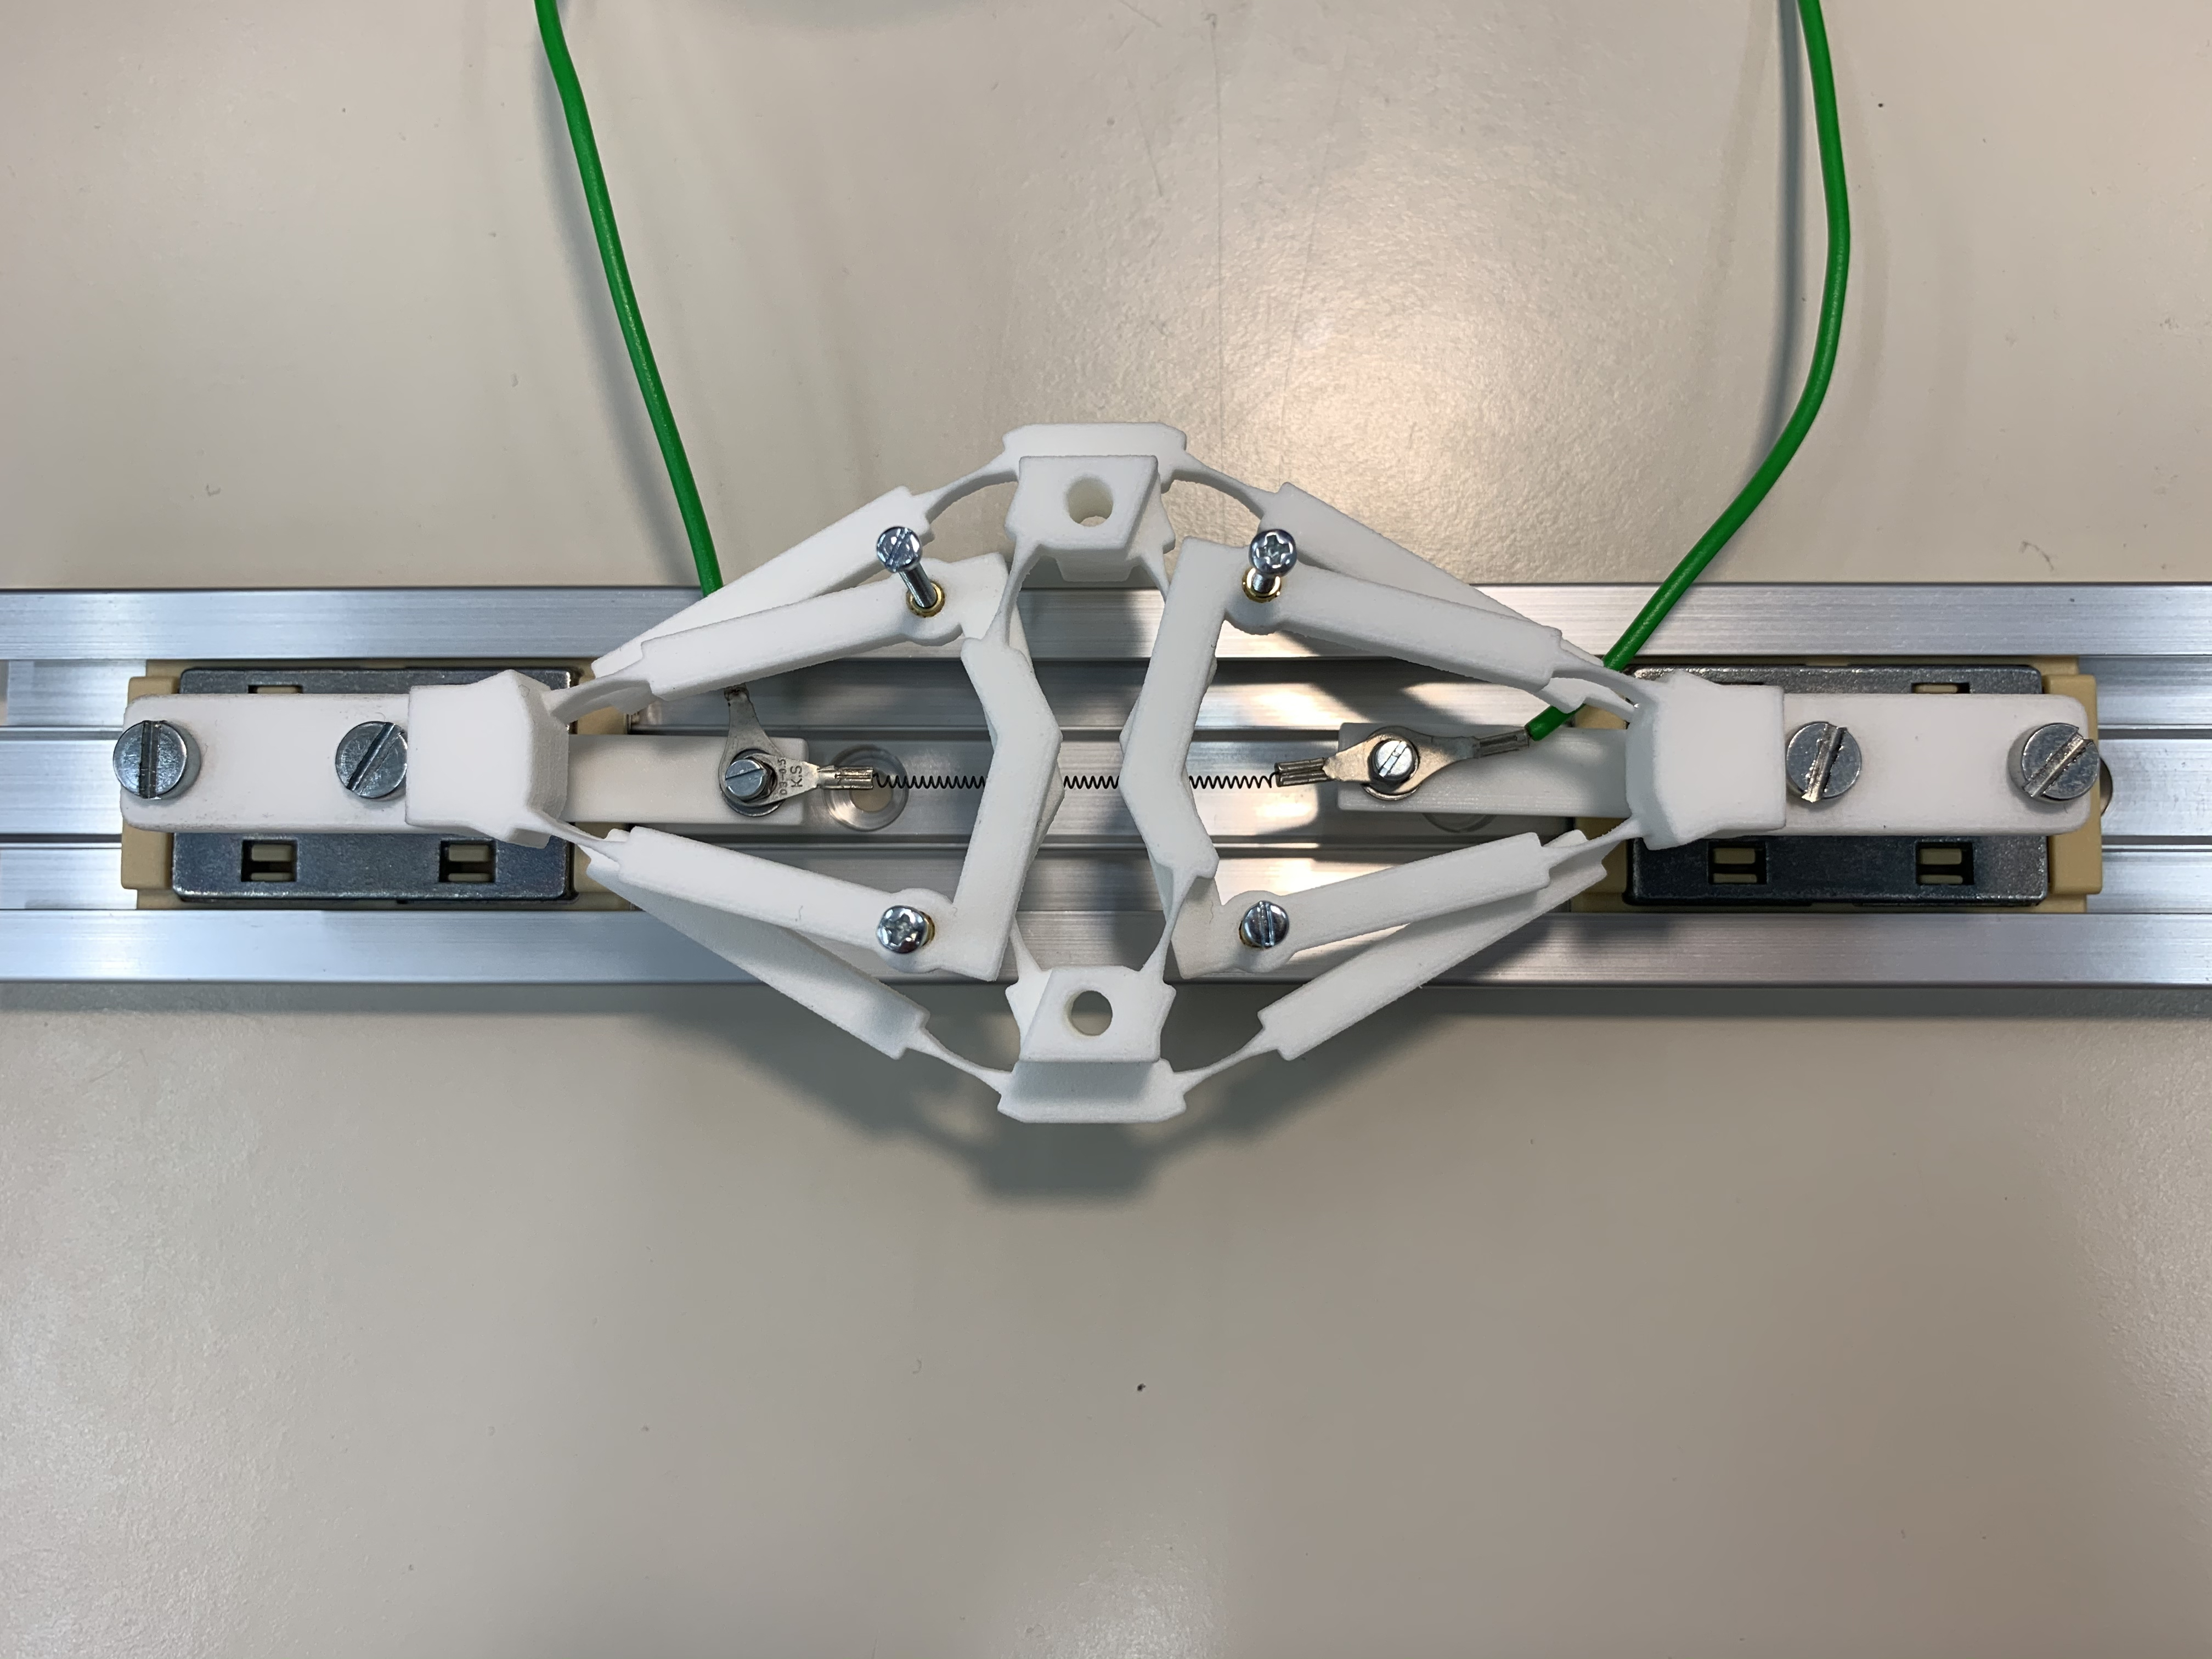
\includegraphics[trim={45cm 50cm 48cm 45cm},clip,width=0.6\columnwidth]{images/chap7/proto_open.jpeg}}}
    \end{overpic}
    }{197.8}{1}{20}};
    \begin{scope}[x={(graph.south east)},y={(graph.north west)}]
       \node[align=left] at (\xFigLetter,\yFigLetter) {\Large \color{white}(a)};
    \end{scope}

     \node[anchor=south west,inner sep=0] (graph1) at (0.06,-3.4){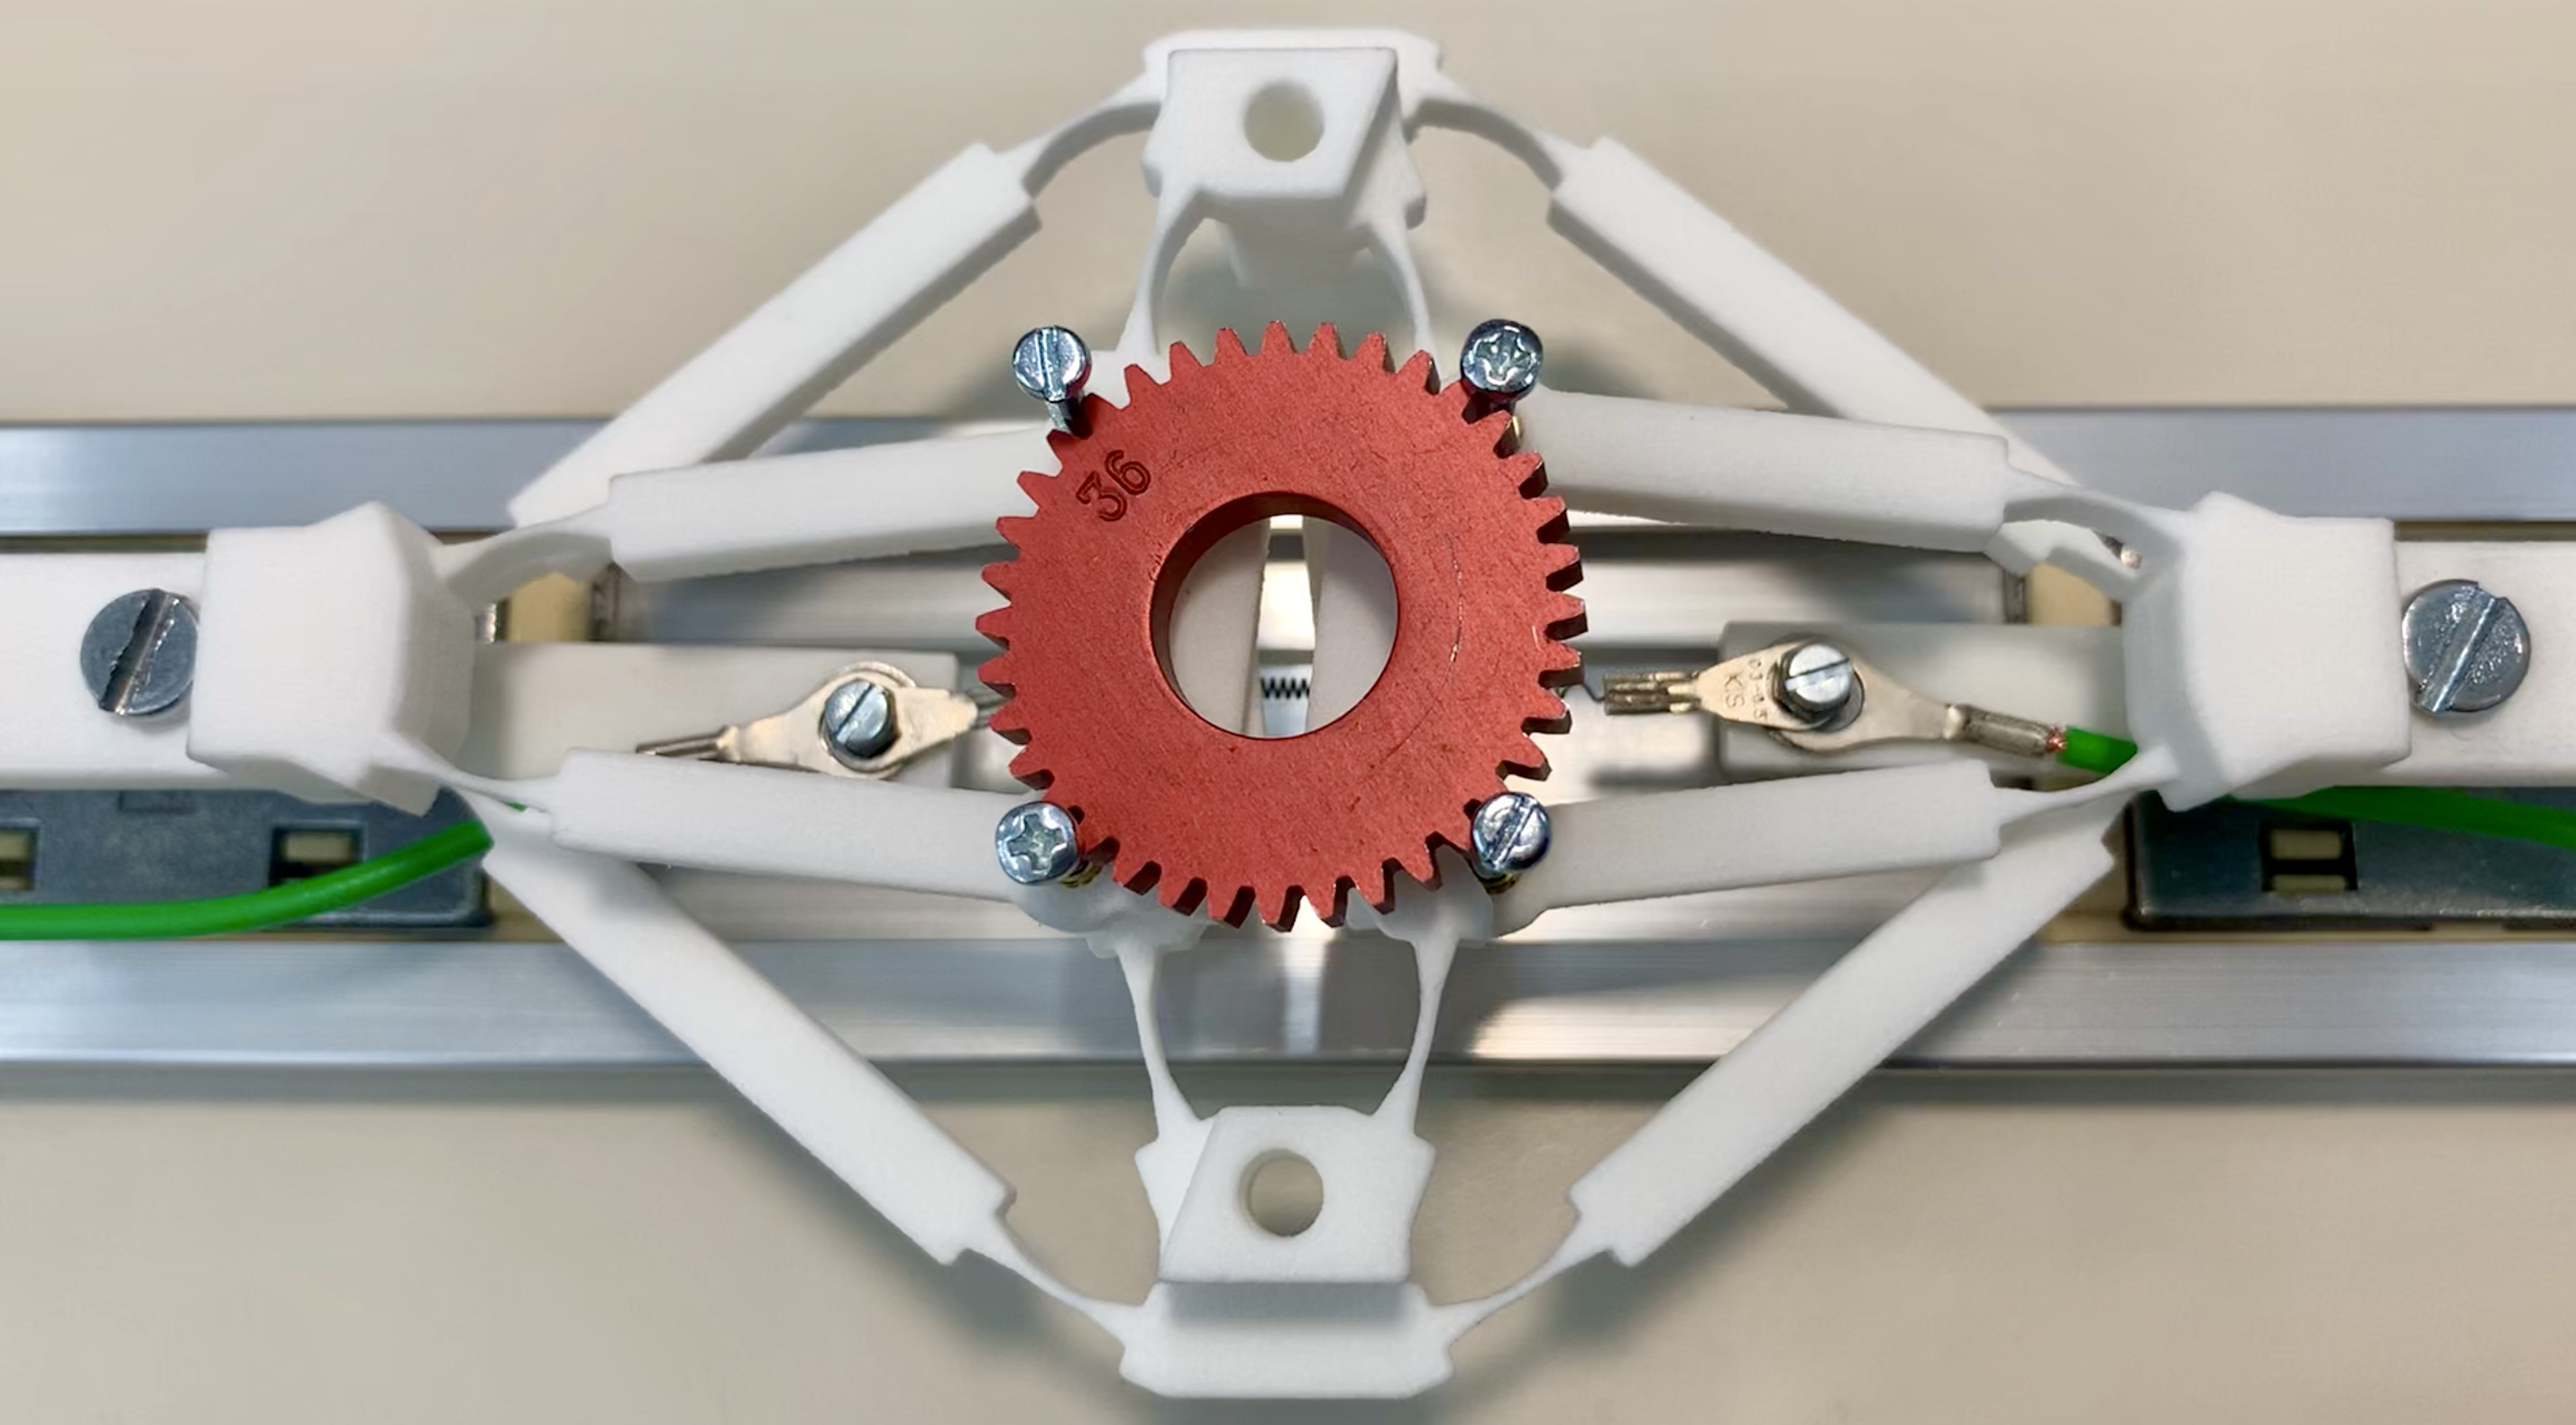
\includegraphics[width=0.98\columnwidth]{images/chap7/closed_with_object.jpeg}};
     \begin{scope}[x={(graph1.south east)},y={(graph1.north west)}]
        \node[align=left] at (\xFigLetter,\yFigLetter) {\Large \color{white}(b)};
     \end{scope}


% \draw[thick,cyan,arrows={-Triangle[angle=90:10pt,cyan,fill=cyan]}] (1.7,\yTopPicture+2.8) -- (3.1,\yTopPicture+2.8);
% \draw[help lines] (0,0) grid (8,4); % $$$$$$$$$$$$$ HELPS A LOT FOR COORDINATES $$$$$$$
 \end{tikzpicture}
\end{document}
}
    \caption{The working prototype of the biased-compliant SMA gripper (a) opened configuration with a $0.2$mm wire diameter SMA coil (framed in red), (b) closed configuration grasping an object.}
    \label{fig:mandrel-finalproto}
\end{figure}

In this prototype, the design parameters used are $e=0.5$ mm, $r=15$ mm, $b=4$ mm, $L_h=42.4$ mm, $x_\text{off}=27.5$ mm and $\theta_0 = \frac{\pi}{8}$. Here, a linear output stroke of up to $4$ mm is observed for each claw. The gripper force, however, is dependant on the size of the gripped object. For an object of diameter close to $x_1$, the gripping force will be maximal. Using a pair of load cells attached to two opposing claws, the gripping force was measured. The load cells were placed at different distances from the claws to simulated objects of varying sizes. The results of the gripper force measurements can be seen in \cref{fig:mandrel-force-temp}. The gripper shows a force close to constant for large span of SMA temperatures above its transition temperature of 80\degreeC. This constant force behaviour is ideal for a gripper and greatly simplifies the control, preventing any unintended damage to the gripped object. A maximum steady-state force of $1.78$ N was measured for the biggest payload size while using the smallest available SMA coil, whose wire diameter is $0.2$ mm. While this result is promising, it should be noted that the fabricated prototype is sub-optimal and can be further optimised for greater forces, either by optimising the compliant mechanism or by using thicker SMA coils. Increasing the wire diameter of the SMA coil comes with higher gripping forces but comes at the cost of slower cooling time or increased time delay between the opening and closing sequence of the gripper.
\begin{figure}[hbt!] % t for top of the page, H could be put to impose the position of the float
  \centering
  \resizebox{0.7\textwidth}{!}{%% Creator: Matplotlib, PGF backend
%%
%% To include the figure in your LaTeX document, write
%%   \input{<filename>.pgf}
%%
%% Make sure the required packages are loaded in your preamble
%%   \usepackage{pgf}
%%
%% Figures using additional raster images can only be included by \input if
%% they are in the same directory as the main LaTeX file. For loading figures
%% from other directories you can use the `import` package
%%   \usepackage{import}
%% and then include the figures with
%%   \import{<path to file>}{<filename>.pgf}
%%
%% Matplotlib used the following preamble
%%
\begingroup%
\makeatletter%
\begin{pgfpicture}%
\pgfpathrectangle{\pgfpointorigin}{\pgfqpoint{5.660000in}{2.780000in}}%
\pgfusepath{use as bounding box, clip}%
\begin{pgfscope}%
\pgfsetbuttcap%
\pgfsetmiterjoin%
\pgfsetlinewidth{0.000000pt}%
\definecolor{currentstroke}{rgb}{0.000000,0.000000,0.000000}%
\pgfsetstrokecolor{currentstroke}%
\pgfsetstrokeopacity{0.000000}%
\pgfsetdash{}{0pt}%
\pgfpathmoveto{\pgfqpoint{0.000000in}{0.000000in}}%
\pgfpathlineto{\pgfqpoint{5.660000in}{0.000000in}}%
\pgfpathlineto{\pgfqpoint{5.660000in}{2.780000in}}%
\pgfpathlineto{\pgfqpoint{0.000000in}{2.780000in}}%
\pgfpathclose%
\pgfusepath{}%
\end{pgfscope}%
\begin{pgfscope}%
\pgfsetbuttcap%
\pgfsetmiterjoin%
\pgfsetlinewidth{0.000000pt}%
\definecolor{currentstroke}{rgb}{0.000000,0.000000,0.000000}%
\pgfsetstrokecolor{currentstroke}%
\pgfsetstrokeopacity{0.000000}%
\pgfsetdash{}{0pt}%
\pgfpathmoveto{\pgfqpoint{0.840504in}{0.670138in}}%
\pgfpathlineto{\pgfqpoint{5.560000in}{0.670138in}}%
\pgfpathlineto{\pgfqpoint{5.560000in}{2.680000in}}%
\pgfpathlineto{\pgfqpoint{0.840504in}{2.680000in}}%
\pgfpathclose%
\pgfusepath{}%
\end{pgfscope}%
\begin{pgfscope}%
\pgfpathrectangle{\pgfqpoint{0.840504in}{0.670138in}}{\pgfqpoint{4.719496in}{2.009862in}}%
\pgfusepath{clip}%
\pgfsetrectcap%
\pgfsetroundjoin%
\pgfsetlinewidth{0.803000pt}%
\definecolor{currentstroke}{rgb}{0.690196,0.690196,0.690196}%
\pgfsetstrokecolor{currentstroke}%
\pgfsetstrokeopacity{0.200000}%
\pgfsetdash{}{0pt}%
\pgfpathmoveto{\pgfqpoint{0.876046in}{0.670138in}}%
\pgfpathlineto{\pgfqpoint{0.876046in}{2.680000in}}%
\pgfusepath{stroke}%
\end{pgfscope}%
\begin{pgfscope}%
\pgfsetbuttcap%
\pgfsetroundjoin%
\definecolor{currentfill}{rgb}{0.000000,0.000000,0.000000}%
\pgfsetfillcolor{currentfill}%
\pgfsetlinewidth{0.803000pt}%
\definecolor{currentstroke}{rgb}{0.000000,0.000000,0.000000}%
\pgfsetstrokecolor{currentstroke}%
\pgfsetdash{}{0pt}%
\pgfsys@defobject{currentmarker}{\pgfqpoint{0.000000in}{-0.048611in}}{\pgfqpoint{0.000000in}{0.000000in}}{%
\pgfpathmoveto{\pgfqpoint{0.000000in}{0.000000in}}%
\pgfpathlineto{\pgfqpoint{0.000000in}{-0.048611in}}%
\pgfusepath{stroke,fill}%
}%
\begin{pgfscope}%
\pgfsys@transformshift{0.876046in}{0.670138in}%
\pgfsys@useobject{currentmarker}{}%
\end{pgfscope}%
\end{pgfscope}%
\begin{pgfscope}%
\definecolor{textcolor}{rgb}{0.000000,0.000000,0.000000}%
\pgfsetstrokecolor{textcolor}%
\pgfsetfillcolor{textcolor}%
\pgftext[x=0.876046in,y=0.572916in,,top]{\color{textcolor}\rmfamily\fontsize{14.000000}{16.800000}\selectfont \(\displaystyle 20\)}%
\end{pgfscope}%
\begin{pgfscope}%
\pgfpathrectangle{\pgfqpoint{0.840504in}{0.670138in}}{\pgfqpoint{4.719496in}{2.009862in}}%
\pgfusepath{clip}%
\pgfsetrectcap%
\pgfsetroundjoin%
\pgfsetlinewidth{0.803000pt}%
\definecolor{currentstroke}{rgb}{0.690196,0.690196,0.690196}%
\pgfsetstrokecolor{currentstroke}%
\pgfsetstrokeopacity{0.200000}%
\pgfsetdash{}{0pt}%
\pgfpathmoveto{\pgfqpoint{1.665058in}{0.670138in}}%
\pgfpathlineto{\pgfqpoint{1.665058in}{2.680000in}}%
\pgfusepath{stroke}%
\end{pgfscope}%
\begin{pgfscope}%
\pgfsetbuttcap%
\pgfsetroundjoin%
\definecolor{currentfill}{rgb}{0.000000,0.000000,0.000000}%
\pgfsetfillcolor{currentfill}%
\pgfsetlinewidth{0.803000pt}%
\definecolor{currentstroke}{rgb}{0.000000,0.000000,0.000000}%
\pgfsetstrokecolor{currentstroke}%
\pgfsetdash{}{0pt}%
\pgfsys@defobject{currentmarker}{\pgfqpoint{0.000000in}{-0.048611in}}{\pgfqpoint{0.000000in}{0.000000in}}{%
\pgfpathmoveto{\pgfqpoint{0.000000in}{0.000000in}}%
\pgfpathlineto{\pgfqpoint{0.000000in}{-0.048611in}}%
\pgfusepath{stroke,fill}%
}%
\begin{pgfscope}%
\pgfsys@transformshift{1.665058in}{0.670138in}%
\pgfsys@useobject{currentmarker}{}%
\end{pgfscope}%
\end{pgfscope}%
\begin{pgfscope}%
\definecolor{textcolor}{rgb}{0.000000,0.000000,0.000000}%
\pgfsetstrokecolor{textcolor}%
\pgfsetfillcolor{textcolor}%
\pgftext[x=1.665058in,y=0.572916in,,top]{\color{textcolor}\rmfamily\fontsize{14.000000}{16.800000}\selectfont \(\displaystyle 40\)}%
\end{pgfscope}%
\begin{pgfscope}%
\pgfpathrectangle{\pgfqpoint{0.840504in}{0.670138in}}{\pgfqpoint{4.719496in}{2.009862in}}%
\pgfusepath{clip}%
\pgfsetrectcap%
\pgfsetroundjoin%
\pgfsetlinewidth{0.803000pt}%
\definecolor{currentstroke}{rgb}{0.690196,0.690196,0.690196}%
\pgfsetstrokecolor{currentstroke}%
\pgfsetstrokeopacity{0.200000}%
\pgfsetdash{}{0pt}%
\pgfpathmoveto{\pgfqpoint{2.454070in}{0.670138in}}%
\pgfpathlineto{\pgfqpoint{2.454070in}{2.680000in}}%
\pgfusepath{stroke}%
\end{pgfscope}%
\begin{pgfscope}%
\pgfsetbuttcap%
\pgfsetroundjoin%
\definecolor{currentfill}{rgb}{0.000000,0.000000,0.000000}%
\pgfsetfillcolor{currentfill}%
\pgfsetlinewidth{0.803000pt}%
\definecolor{currentstroke}{rgb}{0.000000,0.000000,0.000000}%
\pgfsetstrokecolor{currentstroke}%
\pgfsetdash{}{0pt}%
\pgfsys@defobject{currentmarker}{\pgfqpoint{0.000000in}{-0.048611in}}{\pgfqpoint{0.000000in}{0.000000in}}{%
\pgfpathmoveto{\pgfqpoint{0.000000in}{0.000000in}}%
\pgfpathlineto{\pgfqpoint{0.000000in}{-0.048611in}}%
\pgfusepath{stroke,fill}%
}%
\begin{pgfscope}%
\pgfsys@transformshift{2.454070in}{0.670138in}%
\pgfsys@useobject{currentmarker}{}%
\end{pgfscope}%
\end{pgfscope}%
\begin{pgfscope}%
\definecolor{textcolor}{rgb}{0.000000,0.000000,0.000000}%
\pgfsetstrokecolor{textcolor}%
\pgfsetfillcolor{textcolor}%
\pgftext[x=2.454070in,y=0.572916in,,top]{\color{textcolor}\rmfamily\fontsize{14.000000}{16.800000}\selectfont \(\displaystyle 60\)}%
\end{pgfscope}%
\begin{pgfscope}%
\pgfpathrectangle{\pgfqpoint{0.840504in}{0.670138in}}{\pgfqpoint{4.719496in}{2.009862in}}%
\pgfusepath{clip}%
\pgfsetrectcap%
\pgfsetroundjoin%
\pgfsetlinewidth{0.803000pt}%
\definecolor{currentstroke}{rgb}{0.690196,0.690196,0.690196}%
\pgfsetstrokecolor{currentstroke}%
\pgfsetstrokeopacity{0.200000}%
\pgfsetdash{}{0pt}%
\pgfpathmoveto{\pgfqpoint{3.243082in}{0.670138in}}%
\pgfpathlineto{\pgfqpoint{3.243082in}{2.680000in}}%
\pgfusepath{stroke}%
\end{pgfscope}%
\begin{pgfscope}%
\pgfsetbuttcap%
\pgfsetroundjoin%
\definecolor{currentfill}{rgb}{0.000000,0.000000,0.000000}%
\pgfsetfillcolor{currentfill}%
\pgfsetlinewidth{0.803000pt}%
\definecolor{currentstroke}{rgb}{0.000000,0.000000,0.000000}%
\pgfsetstrokecolor{currentstroke}%
\pgfsetdash{}{0pt}%
\pgfsys@defobject{currentmarker}{\pgfqpoint{0.000000in}{-0.048611in}}{\pgfqpoint{0.000000in}{0.000000in}}{%
\pgfpathmoveto{\pgfqpoint{0.000000in}{0.000000in}}%
\pgfpathlineto{\pgfqpoint{0.000000in}{-0.048611in}}%
\pgfusepath{stroke,fill}%
}%
\begin{pgfscope}%
\pgfsys@transformshift{3.243082in}{0.670138in}%
\pgfsys@useobject{currentmarker}{}%
\end{pgfscope}%
\end{pgfscope}%
\begin{pgfscope}%
\definecolor{textcolor}{rgb}{0.000000,0.000000,0.000000}%
\pgfsetstrokecolor{textcolor}%
\pgfsetfillcolor{textcolor}%
\pgftext[x=3.243082in,y=0.572916in,,top]{\color{textcolor}\rmfamily\fontsize{14.000000}{16.800000}\selectfont \(\displaystyle 80\)}%
\end{pgfscope}%
\begin{pgfscope}%
\pgfpathrectangle{\pgfqpoint{0.840504in}{0.670138in}}{\pgfqpoint{4.719496in}{2.009862in}}%
\pgfusepath{clip}%
\pgfsetrectcap%
\pgfsetroundjoin%
\pgfsetlinewidth{0.803000pt}%
\definecolor{currentstroke}{rgb}{0.690196,0.690196,0.690196}%
\pgfsetstrokecolor{currentstroke}%
\pgfsetstrokeopacity{0.200000}%
\pgfsetdash{}{0pt}%
\pgfpathmoveto{\pgfqpoint{4.032094in}{0.670138in}}%
\pgfpathlineto{\pgfqpoint{4.032094in}{2.680000in}}%
\pgfusepath{stroke}%
\end{pgfscope}%
\begin{pgfscope}%
\pgfsetbuttcap%
\pgfsetroundjoin%
\definecolor{currentfill}{rgb}{0.000000,0.000000,0.000000}%
\pgfsetfillcolor{currentfill}%
\pgfsetlinewidth{0.803000pt}%
\definecolor{currentstroke}{rgb}{0.000000,0.000000,0.000000}%
\pgfsetstrokecolor{currentstroke}%
\pgfsetdash{}{0pt}%
\pgfsys@defobject{currentmarker}{\pgfqpoint{0.000000in}{-0.048611in}}{\pgfqpoint{0.000000in}{0.000000in}}{%
\pgfpathmoveto{\pgfqpoint{0.000000in}{0.000000in}}%
\pgfpathlineto{\pgfqpoint{0.000000in}{-0.048611in}}%
\pgfusepath{stroke,fill}%
}%
\begin{pgfscope}%
\pgfsys@transformshift{4.032094in}{0.670138in}%
\pgfsys@useobject{currentmarker}{}%
\end{pgfscope}%
\end{pgfscope}%
\begin{pgfscope}%
\definecolor{textcolor}{rgb}{0.000000,0.000000,0.000000}%
\pgfsetstrokecolor{textcolor}%
\pgfsetfillcolor{textcolor}%
\pgftext[x=4.032094in,y=0.572916in,,top]{\color{textcolor}\rmfamily\fontsize{14.000000}{16.800000}\selectfont \(\displaystyle 100\)}%
\end{pgfscope}%
\begin{pgfscope}%
\pgfpathrectangle{\pgfqpoint{0.840504in}{0.670138in}}{\pgfqpoint{4.719496in}{2.009862in}}%
\pgfusepath{clip}%
\pgfsetrectcap%
\pgfsetroundjoin%
\pgfsetlinewidth{0.803000pt}%
\definecolor{currentstroke}{rgb}{0.690196,0.690196,0.690196}%
\pgfsetstrokecolor{currentstroke}%
\pgfsetstrokeopacity{0.200000}%
\pgfsetdash{}{0pt}%
\pgfpathmoveto{\pgfqpoint{4.821106in}{0.670138in}}%
\pgfpathlineto{\pgfqpoint{4.821106in}{2.680000in}}%
\pgfusepath{stroke}%
\end{pgfscope}%
\begin{pgfscope}%
\pgfsetbuttcap%
\pgfsetroundjoin%
\definecolor{currentfill}{rgb}{0.000000,0.000000,0.000000}%
\pgfsetfillcolor{currentfill}%
\pgfsetlinewidth{0.803000pt}%
\definecolor{currentstroke}{rgb}{0.000000,0.000000,0.000000}%
\pgfsetstrokecolor{currentstroke}%
\pgfsetdash{}{0pt}%
\pgfsys@defobject{currentmarker}{\pgfqpoint{0.000000in}{-0.048611in}}{\pgfqpoint{0.000000in}{0.000000in}}{%
\pgfpathmoveto{\pgfqpoint{0.000000in}{0.000000in}}%
\pgfpathlineto{\pgfqpoint{0.000000in}{-0.048611in}}%
\pgfusepath{stroke,fill}%
}%
\begin{pgfscope}%
\pgfsys@transformshift{4.821106in}{0.670138in}%
\pgfsys@useobject{currentmarker}{}%
\end{pgfscope}%
\end{pgfscope}%
\begin{pgfscope}%
\definecolor{textcolor}{rgb}{0.000000,0.000000,0.000000}%
\pgfsetstrokecolor{textcolor}%
\pgfsetfillcolor{textcolor}%
\pgftext[x=4.821106in,y=0.572916in,,top]{\color{textcolor}\rmfamily\fontsize{14.000000}{16.800000}\selectfont \(\displaystyle 120\)}%
\end{pgfscope}%
\begin{pgfscope}%
\definecolor{textcolor}{rgb}{0.000000,0.000000,0.000000}%
\pgfsetstrokecolor{textcolor}%
\pgfsetfillcolor{textcolor}%
\pgftext[x=3.200252in,y=0.339583in,,top]{\color{textcolor}\rmfamily\fontsize{16.000000}{19.200000}\selectfont Temperature [°C]}%
\end{pgfscope}%
\begin{pgfscope}%
\pgfpathrectangle{\pgfqpoint{0.840504in}{0.670138in}}{\pgfqpoint{4.719496in}{2.009862in}}%
\pgfusepath{clip}%
\pgfsetrectcap%
\pgfsetroundjoin%
\pgfsetlinewidth{0.803000pt}%
\definecolor{currentstroke}{rgb}{0.690196,0.690196,0.690196}%
\pgfsetstrokecolor{currentstroke}%
\pgfsetstrokeopacity{0.200000}%
\pgfsetdash{}{0pt}%
\pgfpathmoveto{\pgfqpoint{0.840504in}{0.803176in}}%
\pgfpathlineto{\pgfqpoint{5.560000in}{0.803176in}}%
\pgfusepath{stroke}%
\end{pgfscope}%
\begin{pgfscope}%
\pgfsetbuttcap%
\pgfsetroundjoin%
\definecolor{currentfill}{rgb}{0.000000,0.000000,0.000000}%
\pgfsetfillcolor{currentfill}%
\pgfsetlinewidth{0.803000pt}%
\definecolor{currentstroke}{rgb}{0.000000,0.000000,0.000000}%
\pgfsetstrokecolor{currentstroke}%
\pgfsetdash{}{0pt}%
\pgfsys@defobject{currentmarker}{\pgfqpoint{-0.048611in}{0.000000in}}{\pgfqpoint{0.000000in}{0.000000in}}{%
\pgfpathmoveto{\pgfqpoint{0.000000in}{0.000000in}}%
\pgfpathlineto{\pgfqpoint{-0.048611in}{0.000000in}}%
\pgfusepath{stroke,fill}%
}%
\begin{pgfscope}%
\pgfsys@transformshift{0.840504in}{0.803176in}%
\pgfsys@useobject{currentmarker}{}%
\end{pgfscope}%
\end{pgfscope}%
\begin{pgfscope}%
\definecolor{textcolor}{rgb}{0.000000,0.000000,0.000000}%
\pgfsetstrokecolor{textcolor}%
\pgfsetfillcolor{textcolor}%
\pgftext[x=0.395138in,y=0.733732in,left,base]{\color{textcolor}\rmfamily\fontsize{14.000000}{16.800000}\selectfont 0.00}%
\end{pgfscope}%
\begin{pgfscope}%
\pgfpathrectangle{\pgfqpoint{0.840504in}{0.670138in}}{\pgfqpoint{4.719496in}{2.009862in}}%
\pgfusepath{clip}%
\pgfsetrectcap%
\pgfsetroundjoin%
\pgfsetlinewidth{0.803000pt}%
\definecolor{currentstroke}{rgb}{0.690196,0.690196,0.690196}%
\pgfsetstrokecolor{currentstroke}%
\pgfsetstrokeopacity{0.200000}%
\pgfsetdash{}{0pt}%
\pgfpathmoveto{\pgfqpoint{0.840504in}{2.606523in}}%
\pgfpathlineto{\pgfqpoint{5.560000in}{2.606523in}}%
\pgfusepath{stroke}%
\end{pgfscope}%
\begin{pgfscope}%
\pgfsetbuttcap%
\pgfsetroundjoin%
\definecolor{currentfill}{rgb}{0.000000,0.000000,0.000000}%
\pgfsetfillcolor{currentfill}%
\pgfsetlinewidth{0.803000pt}%
\definecolor{currentstroke}{rgb}{0.000000,0.000000,0.000000}%
\pgfsetstrokecolor{currentstroke}%
\pgfsetdash{}{0pt}%
\pgfsys@defobject{currentmarker}{\pgfqpoint{-0.048611in}{0.000000in}}{\pgfqpoint{0.000000in}{0.000000in}}{%
\pgfpathmoveto{\pgfqpoint{0.000000in}{0.000000in}}%
\pgfpathlineto{\pgfqpoint{-0.048611in}{0.000000in}}%
\pgfusepath{stroke,fill}%
}%
\begin{pgfscope}%
\pgfsys@transformshift{0.840504in}{2.606523in}%
\pgfsys@useobject{currentmarker}{}%
\end{pgfscope}%
\end{pgfscope}%
\begin{pgfscope}%
\definecolor{textcolor}{rgb}{0.000000,0.000000,0.000000}%
\pgfsetstrokecolor{textcolor}%
\pgfsetfillcolor{textcolor}%
\pgftext[x=0.395138in,y=2.537078in,left,base]{\color{textcolor}\rmfamily\fontsize{14.000000}{16.800000}\selectfont 1.78}%
\end{pgfscope}%
\begin{pgfscope}%
\pgfpathrectangle{\pgfqpoint{0.840504in}{0.670138in}}{\pgfqpoint{4.719496in}{2.009862in}}%
\pgfusepath{clip}%
\pgfsetrectcap%
\pgfsetroundjoin%
\pgfsetlinewidth{0.803000pt}%
\definecolor{currentstroke}{rgb}{0.690196,0.690196,0.690196}%
\pgfsetstrokecolor{currentstroke}%
\pgfsetstrokeopacity{0.200000}%
\pgfsetdash{}{0pt}%
\pgfpathmoveto{\pgfqpoint{0.840504in}{1.899871in}}%
\pgfpathlineto{\pgfqpoint{5.560000in}{1.899871in}}%
\pgfusepath{stroke}%
\end{pgfscope}%
\begin{pgfscope}%
\pgfsetbuttcap%
\pgfsetroundjoin%
\definecolor{currentfill}{rgb}{0.000000,0.000000,0.000000}%
\pgfsetfillcolor{currentfill}%
\pgfsetlinewidth{0.803000pt}%
\definecolor{currentstroke}{rgb}{0.000000,0.000000,0.000000}%
\pgfsetstrokecolor{currentstroke}%
\pgfsetdash{}{0pt}%
\pgfsys@defobject{currentmarker}{\pgfqpoint{-0.048611in}{0.000000in}}{\pgfqpoint{0.000000in}{0.000000in}}{%
\pgfpathmoveto{\pgfqpoint{0.000000in}{0.000000in}}%
\pgfpathlineto{\pgfqpoint{-0.048611in}{0.000000in}}%
\pgfusepath{stroke,fill}%
}%
\begin{pgfscope}%
\pgfsys@transformshift{0.840504in}{1.899871in}%
\pgfsys@useobject{currentmarker}{}%
\end{pgfscope}%
\end{pgfscope}%
\begin{pgfscope}%
\definecolor{textcolor}{rgb}{0.000000,0.000000,0.000000}%
\pgfsetstrokecolor{textcolor}%
\pgfsetfillcolor{textcolor}%
\pgftext[x=0.395138in,y=1.830427in,left,base]{\color{textcolor}\rmfamily\fontsize{14.000000}{16.800000}\selectfont 1.08}%
\end{pgfscope}%
\begin{pgfscope}%
\definecolor{textcolor}{rgb}{0.000000,0.000000,0.000000}%
\pgfsetstrokecolor{textcolor}%
\pgfsetfillcolor{textcolor}%
\pgftext[x=0.339583in,y=1.675069in,,bottom,rotate=90.000000]{\color{textcolor}\rmfamily\fontsize{16.000000}{19.200000}\selectfont Force [N]}%
\end{pgfscope}%
\begin{pgfscope}%
\pgfpathrectangle{\pgfqpoint{0.840504in}{0.670138in}}{\pgfqpoint{4.719496in}{2.009862in}}%
\pgfusepath{clip}%
\pgfsetrectcap%
\pgfsetroundjoin%
\pgfsetlinewidth{2.007500pt}%
\definecolor{currentstroke}{rgb}{0.035294,0.160784,0.619608}%
\pgfsetstrokecolor{currentstroke}%
\pgfsetdash{}{0pt}%
\pgfpathmoveto{\pgfqpoint{1.244869in}{0.761495in}}%
\pgfpathlineto{\pgfqpoint{1.273579in}{0.815516in}}%
\pgfpathlineto{\pgfqpoint{1.303943in}{0.867175in}}%
\pgfpathlineto{\pgfqpoint{1.335895in}{0.916534in}}%
\pgfpathlineto{\pgfqpoint{1.369366in}{0.963653in}}%
\pgfpathlineto{\pgfqpoint{1.404290in}{1.008593in}}%
\pgfpathlineto{\pgfqpoint{1.440599in}{1.051414in}}%
\pgfpathlineto{\pgfqpoint{1.478225in}{1.092177in}}%
\pgfpathlineto{\pgfqpoint{1.517101in}{1.130942in}}%
\pgfpathlineto{\pgfqpoint{1.557159in}{1.167769in}}%
\pgfpathlineto{\pgfqpoint{1.598331in}{1.202720in}}%
\pgfpathlineto{\pgfqpoint{1.640551in}{1.235854in}}%
\pgfpathlineto{\pgfqpoint{1.683749in}{1.267232in}}%
\pgfpathlineto{\pgfqpoint{1.727860in}{1.296915in}}%
\pgfpathlineto{\pgfqpoint{1.772815in}{1.324963in}}%
\pgfpathlineto{\pgfqpoint{1.818547in}{1.351437in}}%
\pgfpathlineto{\pgfqpoint{1.864989in}{1.376397in}}%
\pgfpathlineto{\pgfqpoint{1.912072in}{1.399903in}}%
\pgfpathlineto{\pgfqpoint{1.959729in}{1.422017in}}%
\pgfpathlineto{\pgfqpoint{2.007892in}{1.442798in}}%
\pgfpathlineto{\pgfqpoint{2.056495in}{1.462307in}}%
\pgfpathlineto{\pgfqpoint{2.105469in}{1.480604in}}%
\pgfpathlineto{\pgfqpoint{2.154747in}{1.497751in}}%
\pgfpathlineto{\pgfqpoint{2.204261in}{1.513807in}}%
\pgfpathlineto{\pgfqpoint{2.253944in}{1.528834in}}%
\pgfpathlineto{\pgfqpoint{2.303728in}{1.542890in}}%
\pgfpathlineto{\pgfqpoint{2.350338in}{1.558806in}}%
\pgfpathlineto{\pgfqpoint{2.395594in}{1.573387in}}%
\pgfpathlineto{\pgfqpoint{2.445962in}{1.585983in}}%
\pgfpathlineto{\pgfqpoint{2.496794in}{1.596393in}}%
\pgfpathlineto{\pgfqpoint{2.547602in}{1.604952in}}%
\pgfpathlineto{\pgfqpoint{2.592773in}{1.614257in}}%
\pgfpathlineto{\pgfqpoint{2.634227in}{1.623279in}}%
\pgfpathlineto{\pgfqpoint{2.675183in}{1.631699in}}%
\pgfpathlineto{\pgfqpoint{2.771937in}{1.648148in}}%
\pgfpathlineto{\pgfqpoint{2.961430in}{1.675473in}}%
\pgfpathlineto{\pgfqpoint{3.055382in}{1.690227in}}%
\pgfpathlineto{\pgfqpoint{3.100762in}{1.697079in}}%
\pgfpathlineto{\pgfqpoint{3.145641in}{1.702876in}}%
\pgfpathlineto{\pgfqpoint{3.189491in}{1.708948in}}%
\pgfpathlineto{\pgfqpoint{3.270927in}{1.722680in}}%
\pgfpathlineto{\pgfqpoint{3.307070in}{1.727967in}}%
\pgfpathlineto{\pgfqpoint{3.427264in}{1.746530in}}%
\pgfpathlineto{\pgfqpoint{3.468727in}{1.751562in}}%
\pgfpathlineto{\pgfqpoint{3.549120in}{1.762560in}}%
\pgfpathlineto{\pgfqpoint{3.629549in}{1.770287in}}%
\pgfpathlineto{\pgfqpoint{3.740731in}{1.784666in}}%
\pgfpathlineto{\pgfqpoint{3.819114in}{1.792121in}}%
\pgfpathlineto{\pgfqpoint{3.855916in}{1.794161in}}%
\pgfpathlineto{\pgfqpoint{3.935221in}{1.801321in}}%
\pgfpathlineto{\pgfqpoint{4.014985in}{1.808220in}}%
\pgfpathlineto{\pgfqpoint{4.050009in}{1.810281in}}%
\pgfpathlineto{\pgfqpoint{4.088042in}{1.814551in}}%
\pgfpathlineto{\pgfqpoint{4.162976in}{1.820382in}}%
\pgfpathlineto{\pgfqpoint{4.195995in}{1.822948in}}%
\pgfpathlineto{\pgfqpoint{4.257662in}{1.829458in}}%
\pgfpathlineto{\pgfqpoint{4.291175in}{1.832262in}}%
\pgfpathlineto{\pgfqpoint{4.415510in}{1.840219in}}%
\pgfpathlineto{\pgfqpoint{4.447220in}{1.842774in}}%
\pgfpathlineto{\pgfqpoint{4.536476in}{1.847913in}}%
\pgfpathlineto{\pgfqpoint{4.564100in}{1.849289in}}%
\pgfpathlineto{\pgfqpoint{4.624996in}{1.853569in}}%
\pgfpathlineto{\pgfqpoint{4.654524in}{1.855442in}}%
\pgfpathlineto{\pgfqpoint{4.710133in}{1.859724in}}%
\pgfpathlineto{\pgfqpoint{4.762426in}{1.862614in}}%
\pgfpathlineto{\pgfqpoint{4.787336in}{1.864811in}}%
\pgfpathlineto{\pgfqpoint{4.838465in}{1.866683in}}%
\pgfpathlineto{\pgfqpoint{4.864933in}{1.868916in}}%
\pgfpathlineto{\pgfqpoint{4.917629in}{1.872259in}}%
\pgfpathlineto{\pgfqpoint{5.002447in}{1.875361in}}%
\pgfpathlineto{\pgfqpoint{5.031476in}{1.877004in}}%
\pgfpathlineto{\pgfqpoint{5.086410in}{1.878979in}}%
\pgfpathlineto{\pgfqpoint{5.192093in}{1.885596in}}%
\pgfpathlineto{\pgfqpoint{5.214166in}{1.887479in}}%
\pgfpathlineto{\pgfqpoint{5.277533in}{1.888224in}}%
\pgfpathlineto{\pgfqpoint{5.295207in}{1.889191in}}%
\pgfpathlineto{\pgfqpoint{5.310983in}{1.888994in}}%
\pgfpathlineto{\pgfqpoint{5.322916in}{1.890764in}}%
\pgfpathlineto{\pgfqpoint{5.332634in}{1.890571in}}%
\pgfpathlineto{\pgfqpoint{5.345394in}{1.890945in}}%
\pgfpathlineto{\pgfqpoint{5.345477in}{1.891401in}}%
\pgfpathlineto{\pgfqpoint{5.345111in}{1.892275in}}%
\pgfpathlineto{\pgfqpoint{5.341200in}{1.892042in}}%
\pgfpathlineto{\pgfqpoint{5.329432in}{1.892513in}}%
\pgfpathlineto{\pgfqpoint{5.311454in}{1.892893in}}%
\pgfpathlineto{\pgfqpoint{5.267046in}{1.890788in}}%
\pgfpathlineto{\pgfqpoint{5.225624in}{1.889693in}}%
\pgfpathlineto{\pgfqpoint{5.201350in}{1.889618in}}%
\pgfpathlineto{\pgfqpoint{5.175322in}{1.888614in}}%
\pgfpathlineto{\pgfqpoint{5.150072in}{1.888104in}}%
\pgfpathlineto{\pgfqpoint{5.121641in}{1.887993in}}%
\pgfpathlineto{\pgfqpoint{5.090239in}{1.888285in}}%
\pgfpathlineto{\pgfqpoint{5.059826in}{1.888098in}}%
\pgfpathlineto{\pgfqpoint{5.030348in}{1.887438in}}%
\pgfpathlineto{\pgfqpoint{4.965569in}{1.888061in}}%
\pgfpathlineto{\pgfqpoint{4.898611in}{1.885637in}}%
\pgfpathlineto{\pgfqpoint{4.834092in}{1.885145in}}%
\pgfpathlineto{\pgfqpoint{4.801923in}{1.883820in}}%
\pgfpathlineto{\pgfqpoint{4.770246in}{1.882943in}}%
\pgfpathlineto{\pgfqpoint{4.740257in}{1.882613in}}%
\pgfpathlineto{\pgfqpoint{4.710588in}{1.881759in}}%
\pgfpathlineto{\pgfqpoint{4.680060in}{1.881367in}}%
\pgfpathlineto{\pgfqpoint{4.652785in}{1.880461in}}%
\pgfpathlineto{\pgfqpoint{4.625911in}{1.880030in}}%
\pgfpathlineto{\pgfqpoint{4.599703in}{1.880080in}}%
\pgfpathlineto{\pgfqpoint{4.572779in}{1.879196in}}%
\pgfpathlineto{\pgfqpoint{4.546131in}{1.878808in}}%
\pgfpathlineto{\pgfqpoint{4.520135in}{1.877940in}}%
\pgfpathlineto{\pgfqpoint{4.497001in}{1.878120in}}%
\pgfpathlineto{\pgfqpoint{4.471534in}{1.877740in}}%
\pgfpathlineto{\pgfqpoint{4.446636in}{1.876806in}}%
\pgfpathlineto{\pgfqpoint{4.421302in}{1.876307in}}%
\pgfpathlineto{\pgfqpoint{4.396240in}{1.875266in}}%
\pgfpathlineto{\pgfqpoint{4.373412in}{1.875114in}}%
\pgfpathlineto{\pgfqpoint{4.300842in}{1.873052in}}%
\pgfpathlineto{\pgfqpoint{4.275139in}{1.871725in}}%
\pgfpathlineto{\pgfqpoint{4.249548in}{1.871326in}}%
\pgfpathlineto{\pgfqpoint{4.224340in}{1.870438in}}%
\pgfpathlineto{\pgfqpoint{4.175048in}{1.869737in}}%
\pgfpathlineto{\pgfqpoint{4.150614in}{1.869849in}}%
\pgfpathlineto{\pgfqpoint{4.128205in}{1.869326in}}%
\pgfpathlineto{\pgfqpoint{4.106338in}{1.868274in}}%
\pgfpathlineto{\pgfqpoint{4.085325in}{1.867684in}}%
\pgfpathlineto{\pgfqpoint{4.062478in}{1.866585in}}%
\pgfpathlineto{\pgfqpoint{4.039498in}{1.864983in}}%
\pgfpathlineto{\pgfqpoint{4.016700in}{1.863867in}}%
\pgfpathlineto{\pgfqpoint{3.974763in}{1.861052in}}%
\pgfpathlineto{\pgfqpoint{3.951793in}{1.859713in}}%
\pgfpathlineto{\pgfqpoint{3.929238in}{1.859330in}}%
\pgfpathlineto{\pgfqpoint{3.865692in}{1.856814in}}%
\pgfpathlineto{\pgfqpoint{3.845889in}{1.856985in}}%
\pgfpathlineto{\pgfqpoint{3.803097in}{1.855395in}}%
\pgfpathlineto{\pgfqpoint{3.783938in}{1.853559in}}%
\pgfpathlineto{\pgfqpoint{3.765287in}{1.854105in}}%
\pgfpathlineto{\pgfqpoint{3.743890in}{1.853563in}}%
\pgfpathlineto{\pgfqpoint{3.722805in}{1.852392in}}%
\pgfpathlineto{\pgfqpoint{3.702333in}{1.849524in}}%
\pgfpathlineto{\pgfqpoint{3.682159in}{1.848990in}}%
\pgfpathlineto{\pgfqpoint{3.663240in}{1.847953in}}%
\pgfpathlineto{\pgfqpoint{3.624764in}{1.844874in}}%
\pgfpathlineto{\pgfqpoint{3.586910in}{1.843398in}}%
\pgfpathlineto{\pgfqpoint{3.551823in}{1.840714in}}%
\pgfpathlineto{\pgfqpoint{3.516902in}{1.837038in}}%
\pgfpathlineto{\pgfqpoint{3.500697in}{1.836187in}}%
\pgfpathlineto{\pgfqpoint{3.485541in}{1.834248in}}%
\pgfpathlineto{\pgfqpoint{3.468900in}{1.833297in}}%
\pgfpathlineto{\pgfqpoint{3.452718in}{1.831385in}}%
\pgfpathlineto{\pgfqpoint{3.437179in}{1.830490in}}%
\pgfpathlineto{\pgfqpoint{3.405388in}{1.827251in}}%
\pgfpathlineto{\pgfqpoint{3.390960in}{1.826264in}}%
\pgfpathlineto{\pgfqpoint{3.375150in}{1.823851in}}%
\pgfpathlineto{\pgfqpoint{3.359760in}{1.823415in}}%
\pgfpathlineto{\pgfqpoint{3.342973in}{1.820948in}}%
\pgfpathlineto{\pgfqpoint{3.328008in}{1.819504in}}%
\pgfpathlineto{\pgfqpoint{3.313318in}{1.817671in}}%
\pgfpathlineto{\pgfqpoint{3.283701in}{1.815009in}}%
\pgfpathlineto{\pgfqpoint{3.256733in}{1.813143in}}%
\pgfpathlineto{\pgfqpoint{3.218713in}{1.808701in}}%
\pgfpathlineto{\pgfqpoint{3.191554in}{1.806439in}}%
\pgfpathlineto{\pgfqpoint{3.179380in}{1.804433in}}%
\pgfpathlineto{\pgfqpoint{3.140564in}{1.800695in}}%
\pgfpathlineto{\pgfqpoint{3.127548in}{1.798802in}}%
\pgfpathlineto{\pgfqpoint{3.114511in}{1.797919in}}%
\pgfpathlineto{\pgfqpoint{3.101587in}{1.796449in}}%
\pgfpathlineto{\pgfqpoint{3.075949in}{1.794238in}}%
\pgfpathlineto{\pgfqpoint{3.051318in}{1.790915in}}%
\pgfpathlineto{\pgfqpoint{3.039761in}{1.788342in}}%
\pgfpathlineto{\pgfqpoint{3.014552in}{1.785285in}}%
\pgfpathlineto{\pgfqpoint{3.001382in}{1.784298in}}%
\pgfpathlineto{\pgfqpoint{2.976199in}{1.778931in}}%
\pgfpathlineto{\pgfqpoint{2.964282in}{1.776981in}}%
\pgfpathlineto{\pgfqpoint{2.951168in}{1.775984in}}%
\pgfpathlineto{\pgfqpoint{2.938161in}{1.773992in}}%
\pgfpathlineto{\pgfqpoint{2.925501in}{1.772451in}}%
\pgfpathlineto{\pgfqpoint{2.912901in}{1.770489in}}%
\pgfpathlineto{\pgfqpoint{2.900479in}{1.769108in}}%
\pgfpathlineto{\pgfqpoint{2.888412in}{1.766705in}}%
\pgfpathlineto{\pgfqpoint{2.875277in}{1.764719in}}%
\pgfpathlineto{\pgfqpoint{2.850994in}{1.762320in}}%
\pgfpathlineto{\pgfqpoint{2.828894in}{1.759671in}}%
\pgfpathlineto{\pgfqpoint{2.816346in}{1.757374in}}%
\pgfpathlineto{\pgfqpoint{2.790971in}{1.753681in}}%
\pgfpathlineto{\pgfqpoint{2.779080in}{1.750991in}}%
\pgfpathlineto{\pgfqpoint{2.767478in}{1.750316in}}%
\pgfpathlineto{\pgfqpoint{2.755107in}{1.748191in}}%
\pgfpathlineto{\pgfqpoint{2.731793in}{1.744921in}}%
\pgfpathlineto{\pgfqpoint{2.720693in}{1.744257in}}%
\pgfpathlineto{\pgfqpoint{2.699458in}{1.741306in}}%
\pgfpathlineto{\pgfqpoint{2.668922in}{1.737746in}}%
\pgfpathlineto{\pgfqpoint{2.638502in}{1.733496in}}%
\pgfpathlineto{\pgfqpoint{2.628115in}{1.732931in}}%
\pgfpathlineto{\pgfqpoint{2.617852in}{1.731878in}}%
\pgfpathlineto{\pgfqpoint{2.598673in}{1.728105in}}%
\pgfpathlineto{\pgfqpoint{2.578059in}{1.724252in}}%
\pgfpathlineto{\pgfqpoint{2.559560in}{1.719769in}}%
\pgfpathlineto{\pgfqpoint{2.550863in}{1.718168in}}%
\pgfpathlineto{\pgfqpoint{2.540944in}{1.717117in}}%
\pgfpathlineto{\pgfqpoint{2.522074in}{1.712796in}}%
\pgfpathlineto{\pgfqpoint{2.513357in}{1.710006in}}%
\pgfpathlineto{\pgfqpoint{2.495211in}{1.705472in}}%
\pgfpathlineto{\pgfqpoint{2.485742in}{1.703769in}}%
\pgfpathlineto{\pgfqpoint{2.478420in}{1.701587in}}%
\pgfpathlineto{\pgfqpoint{2.471274in}{1.699935in}}%
\pgfpathlineto{\pgfqpoint{2.465833in}{1.697661in}}%
\pgfpathlineto{\pgfqpoint{2.459553in}{1.696217in}}%
\pgfpathlineto{\pgfqpoint{2.453268in}{1.694204in}}%
\pgfpathlineto{\pgfqpoint{2.445917in}{1.692286in}}%
\pgfpathlineto{\pgfqpoint{2.438808in}{1.689948in}}%
\pgfpathlineto{\pgfqpoint{2.417552in}{1.684233in}}%
\pgfpathlineto{\pgfqpoint{2.410316in}{1.681572in}}%
\pgfpathlineto{\pgfqpoint{2.404095in}{1.679952in}}%
\pgfpathlineto{\pgfqpoint{2.384256in}{1.672885in}}%
\pgfpathlineto{\pgfqpoint{2.376341in}{1.669917in}}%
\pgfpathlineto{\pgfqpoint{2.368236in}{1.667733in}}%
\pgfpathlineto{\pgfqpoint{2.352244in}{1.662090in}}%
\pgfpathlineto{\pgfqpoint{2.327866in}{1.655230in}}%
\pgfpathlineto{\pgfqpoint{2.319967in}{1.651407in}}%
\pgfpathlineto{\pgfqpoint{2.312147in}{1.649104in}}%
\pgfpathlineto{\pgfqpoint{2.296139in}{1.643620in}}%
\pgfpathlineto{\pgfqpoint{2.287753in}{1.641283in}}%
\pgfpathlineto{\pgfqpoint{2.279933in}{1.637879in}}%
\pgfpathlineto{\pgfqpoint{2.272172in}{1.634954in}}%
\pgfpathlineto{\pgfqpoint{2.263077in}{1.632092in}}%
\pgfpathlineto{\pgfqpoint{2.253961in}{1.630747in}}%
\pgfpathlineto{\pgfqpoint{2.245074in}{1.628795in}}%
\pgfpathlineto{\pgfqpoint{2.236150in}{1.625828in}}%
\pgfpathlineto{\pgfqpoint{2.227514in}{1.623394in}}%
\pgfpathlineto{\pgfqpoint{2.209706in}{1.616656in}}%
\pgfpathlineto{\pgfqpoint{2.200553in}{1.613381in}}%
\pgfpathlineto{\pgfqpoint{2.192450in}{1.611181in}}%
\pgfpathlineto{\pgfqpoint{2.184278in}{1.608025in}}%
\pgfpathlineto{\pgfqpoint{2.168127in}{1.603568in}}%
\pgfpathlineto{\pgfqpoint{2.159425in}{1.601884in}}%
\pgfpathlineto{\pgfqpoint{2.136116in}{1.595328in}}%
\pgfpathlineto{\pgfqpoint{2.128689in}{1.592201in}}%
\pgfpathlineto{\pgfqpoint{2.109055in}{1.586183in}}%
\pgfpathlineto{\pgfqpoint{2.092893in}{1.578959in}}%
\pgfpathlineto{\pgfqpoint{2.080024in}{1.574883in}}%
\pgfpathlineto{\pgfqpoint{2.067779in}{1.569986in}}%
\pgfpathlineto{\pgfqpoint{2.061841in}{1.568542in}}%
\pgfpathlineto{\pgfqpoint{2.055857in}{1.566202in}}%
\pgfpathlineto{\pgfqpoint{2.050613in}{1.562994in}}%
\pgfpathlineto{\pgfqpoint{2.045581in}{1.561695in}}%
\pgfpathlineto{\pgfqpoint{2.040209in}{1.558308in}}%
\pgfpathlineto{\pgfqpoint{2.034992in}{1.556979in}}%
\pgfpathlineto{\pgfqpoint{2.028861in}{1.553807in}}%
\pgfpathlineto{\pgfqpoint{2.022785in}{1.552110in}}%
\pgfpathlineto{\pgfqpoint{2.016821in}{1.550837in}}%
\pgfpathlineto{\pgfqpoint{2.011986in}{1.548056in}}%
\pgfpathlineto{\pgfqpoint{2.006625in}{1.546200in}}%
\pgfpathlineto{\pgfqpoint{2.001295in}{1.543680in}}%
\pgfpathlineto{\pgfqpoint{1.990283in}{1.539263in}}%
\pgfpathlineto{\pgfqpoint{1.980052in}{1.533163in}}%
\pgfpathlineto{\pgfqpoint{1.974501in}{1.530338in}}%
\pgfpathlineto{\pgfqpoint{1.969056in}{1.528536in}}%
\pgfpathlineto{\pgfqpoint{1.959256in}{1.524000in}}%
\pgfpathlineto{\pgfqpoint{1.954319in}{1.521674in}}%
\pgfpathlineto{\pgfqpoint{1.940461in}{1.514155in}}%
\pgfpathlineto{\pgfqpoint{1.935813in}{1.511697in}}%
\pgfpathlineto{\pgfqpoint{1.926482in}{1.504183in}}%
\pgfpathlineto{\pgfqpoint{1.922299in}{1.502024in}}%
\pgfpathlineto{\pgfqpoint{1.917934in}{1.498855in}}%
\pgfpathlineto{\pgfqpoint{1.913693in}{1.497557in}}%
\pgfpathlineto{\pgfqpoint{1.909630in}{1.494776in}}%
\pgfpathlineto{\pgfqpoint{1.897073in}{1.488147in}}%
\pgfpathlineto{\pgfqpoint{1.892469in}{1.484492in}}%
\pgfpathlineto{\pgfqpoint{1.888168in}{1.481825in}}%
\pgfpathlineto{\pgfqpoint{1.883939in}{1.478652in}}%
\pgfpathlineto{\pgfqpoint{1.869092in}{1.470080in}}%
\pgfpathlineto{\pgfqpoint{1.860126in}{1.464840in}}%
\pgfpathlineto{\pgfqpoint{1.852057in}{1.458256in}}%
\pgfpathlineto{\pgfqpoint{1.847997in}{1.455507in}}%
\pgfpathlineto{\pgfqpoint{1.843980in}{1.452325in}}%
\pgfpathlineto{\pgfqpoint{1.840030in}{1.451146in}}%
\pgfpathlineto{\pgfqpoint{1.836214in}{1.447980in}}%
\pgfpathlineto{\pgfqpoint{1.828235in}{1.442844in}}%
\pgfpathlineto{\pgfqpoint{1.819968in}{1.437070in}}%
\pgfpathlineto{\pgfqpoint{1.817058in}{1.434221in}}%
\pgfpathlineto{\pgfqpoint{1.813613in}{1.432519in}}%
\pgfpathlineto{\pgfqpoint{1.810146in}{1.428856in}}%
\pgfpathlineto{\pgfqpoint{1.806432in}{1.427096in}}%
\pgfpathlineto{\pgfqpoint{1.802711in}{1.424419in}}%
\pgfpathlineto{\pgfqpoint{1.799047in}{1.423268in}}%
\pgfpathlineto{\pgfqpoint{1.795745in}{1.420193in}}%
\pgfpathlineto{\pgfqpoint{1.792543in}{1.416648in}}%
\pgfpathlineto{\pgfqpoint{1.788606in}{1.413735in}}%
\pgfpathlineto{\pgfqpoint{1.776503in}{1.406647in}}%
\pgfpathlineto{\pgfqpoint{1.764679in}{1.398528in}}%
\pgfpathlineto{\pgfqpoint{1.760810in}{1.396448in}}%
\pgfpathlineto{\pgfqpoint{1.757597in}{1.393433in}}%
\pgfpathlineto{\pgfqpoint{1.754463in}{1.391381in}}%
\pgfpathlineto{\pgfqpoint{1.744721in}{1.382885in}}%
\pgfpathlineto{\pgfqpoint{1.741055in}{1.380586in}}%
\pgfpathlineto{\pgfqpoint{1.737389in}{1.377785in}}%
\pgfpathlineto{\pgfqpoint{1.733762in}{1.375495in}}%
\pgfpathlineto{\pgfqpoint{1.727229in}{1.370172in}}%
\pgfpathlineto{\pgfqpoint{1.723515in}{1.367643in}}%
\pgfpathlineto{\pgfqpoint{1.719835in}{1.364669in}}%
\pgfpathlineto{\pgfqpoint{1.716737in}{1.361626in}}%
\pgfpathlineto{\pgfqpoint{1.713642in}{1.359427in}}%
\pgfpathlineto{\pgfqpoint{1.709994in}{1.355791in}}%
\pgfpathlineto{\pgfqpoint{1.702712in}{1.349665in}}%
\pgfpathlineto{\pgfqpoint{1.699149in}{1.348116in}}%
\pgfpathlineto{\pgfqpoint{1.689285in}{1.340234in}}%
\pgfpathlineto{\pgfqpoint{1.683171in}{1.334327in}}%
\pgfpathlineto{\pgfqpoint{1.680392in}{1.332865in}}%
\pgfpathlineto{\pgfqpoint{1.677374in}{1.330759in}}%
\pgfpathlineto{\pgfqpoint{1.674330in}{1.328138in}}%
\pgfpathlineto{\pgfqpoint{1.670766in}{1.325671in}}%
\pgfpathlineto{\pgfqpoint{1.667201in}{1.323735in}}%
\pgfpathlineto{\pgfqpoint{1.660983in}{1.318981in}}%
\pgfpathlineto{\pgfqpoint{1.646419in}{1.305337in}}%
\pgfpathlineto{\pgfqpoint{1.639529in}{1.299911in}}%
\pgfpathlineto{\pgfqpoint{1.635983in}{1.298434in}}%
\pgfpathlineto{\pgfqpoint{1.632652in}{1.295370in}}%
\pgfpathlineto{\pgfqpoint{1.629328in}{1.293254in}}%
\pgfpathlineto{\pgfqpoint{1.625962in}{1.289612in}}%
\pgfpathlineto{\pgfqpoint{1.614916in}{1.282976in}}%
\pgfpathlineto{\pgfqpoint{1.611367in}{1.280249in}}%
\pgfpathlineto{\pgfqpoint{1.607835in}{1.276936in}}%
\pgfpathlineto{\pgfqpoint{1.604359in}{1.274486in}}%
\pgfpathlineto{\pgfqpoint{1.592507in}{1.264384in}}%
\pgfpathlineto{\pgfqpoint{1.582428in}{1.257217in}}%
\pgfpathlineto{\pgfqpoint{1.578889in}{1.253685in}}%
\pgfpathlineto{\pgfqpoint{1.575932in}{1.251623in}}%
\pgfpathlineto{\pgfqpoint{1.572983in}{1.249003in}}%
\pgfpathlineto{\pgfqpoint{1.567309in}{1.242300in}}%
\pgfpathlineto{\pgfqpoint{1.564335in}{1.240677in}}%
\pgfpathlineto{\pgfqpoint{1.561463in}{1.238516in}}%
\pgfpathlineto{\pgfqpoint{1.558726in}{1.234962in}}%
\pgfpathlineto{\pgfqpoint{1.550588in}{1.227183in}}%
\pgfpathlineto{\pgfqpoint{1.546121in}{1.222551in}}%
\pgfpathlineto{\pgfqpoint{1.544256in}{1.220825in}}%
\pgfpathlineto{\pgfqpoint{1.542452in}{1.217179in}}%
\pgfpathlineto{\pgfqpoint{1.537936in}{1.212972in}}%
\pgfpathlineto{\pgfqpoint{1.533982in}{1.208182in}}%
\pgfpathlineto{\pgfqpoint{1.531936in}{1.206832in}}%
\pgfpathlineto{\pgfqpoint{1.527744in}{1.200977in}}%
\pgfpathlineto{\pgfqpoint{1.523573in}{1.196977in}}%
\pgfpathlineto{\pgfqpoint{1.521641in}{1.194071in}}%
\pgfpathlineto{\pgfqpoint{1.519263in}{1.193090in}}%
\pgfpathlineto{\pgfqpoint{1.517150in}{1.190482in}}%
\pgfpathlineto{\pgfqpoint{1.515079in}{1.188784in}}%
\pgfpathlineto{\pgfqpoint{1.511511in}{1.183764in}}%
\pgfpathlineto{\pgfqpoint{1.507588in}{1.179152in}}%
\pgfpathlineto{\pgfqpoint{1.505355in}{1.176356in}}%
\pgfpathlineto{\pgfqpoint{1.503152in}{1.174646in}}%
\pgfpathlineto{\pgfqpoint{1.500982in}{1.171355in}}%
\pgfpathlineto{\pgfqpoint{1.498567in}{1.169362in}}%
\pgfpathlineto{\pgfqpoint{1.496174in}{1.166289in}}%
\pgfpathlineto{\pgfqpoint{1.493882in}{1.164130in}}%
\pgfpathlineto{\pgfqpoint{1.489909in}{1.159097in}}%
\pgfpathlineto{\pgfqpoint{1.485885in}{1.154082in}}%
\pgfpathlineto{\pgfqpoint{1.480775in}{1.145038in}}%
\pgfpathlineto{\pgfqpoint{1.478708in}{1.142883in}}%
\pgfpathlineto{\pgfqpoint{1.472868in}{1.134467in}}%
\pgfpathlineto{\pgfqpoint{1.468159in}{1.125364in}}%
\pgfpathlineto{\pgfqpoint{1.464227in}{1.118442in}}%
\pgfpathlineto{\pgfqpoint{1.459900in}{1.113576in}}%
\pgfpathlineto{\pgfqpoint{1.455992in}{1.106428in}}%
\pgfpathlineto{\pgfqpoint{1.453019in}{1.102370in}}%
\pgfpathlineto{\pgfqpoint{1.449490in}{1.094353in}}%
\pgfpathlineto{\pgfqpoint{1.446367in}{1.088748in}}%
\pgfpathlineto{\pgfqpoint{1.444861in}{1.087419in}}%
\pgfpathlineto{\pgfqpoint{1.443351in}{1.084676in}}%
\pgfpathlineto{\pgfqpoint{1.440344in}{1.081662in}}%
\pgfpathlineto{\pgfqpoint{1.438575in}{1.079495in}}%
\pgfpathlineto{\pgfqpoint{1.433926in}{1.071750in}}%
\pgfpathlineto{\pgfqpoint{1.432364in}{1.069827in}}%
\pgfpathlineto{\pgfqpoint{1.430802in}{1.067074in}}%
\pgfpathlineto{\pgfqpoint{1.429267in}{1.065926in}}%
\pgfpathlineto{\pgfqpoint{1.427787in}{1.063273in}}%
\pgfpathlineto{\pgfqpoint{1.426094in}{1.061453in}}%
\pgfpathlineto{\pgfqpoint{1.424440in}{1.058625in}}%
\pgfpathlineto{\pgfqpoint{1.419300in}{1.051854in}}%
\pgfpathlineto{\pgfqpoint{1.416038in}{1.047139in}}%
\pgfpathlineto{\pgfqpoint{1.411739in}{1.040068in}}%
\pgfpathlineto{\pgfqpoint{1.405452in}{1.028199in}}%
\pgfpathlineto{\pgfqpoint{1.402822in}{1.024936in}}%
\pgfpathlineto{\pgfqpoint{1.401448in}{1.022685in}}%
\pgfpathlineto{\pgfqpoint{1.399830in}{1.020973in}}%
\pgfpathlineto{\pgfqpoint{1.398476in}{1.018300in}}%
\pgfpathlineto{\pgfqpoint{1.395743in}{1.014540in}}%
\pgfpathlineto{\pgfqpoint{1.391431in}{1.008363in}}%
\pgfpathlineto{\pgfqpoint{1.383283in}{0.998234in}}%
\pgfpathlineto{\pgfqpoint{1.380964in}{0.993064in}}%
\pgfpathlineto{\pgfqpoint{1.379942in}{0.991461in}}%
\pgfpathlineto{\pgfqpoint{1.378458in}{0.988289in}}%
\pgfpathlineto{\pgfqpoint{1.360959in}{0.955278in}}%
\pgfpathlineto{\pgfqpoint{1.353718in}{0.946637in}}%
\pgfpathlineto{\pgfqpoint{1.352073in}{0.946353in}}%
\pgfpathlineto{\pgfqpoint{1.344409in}{0.939085in}}%
\pgfpathlineto{\pgfqpoint{1.343344in}{0.939314in}}%
\pgfpathlineto{\pgfqpoint{1.341566in}{0.936859in}}%
\pgfpathlineto{\pgfqpoint{1.338497in}{0.934230in}}%
\pgfpathlineto{\pgfqpoint{1.337512in}{0.933265in}}%
\pgfpathlineto{\pgfqpoint{1.336528in}{0.932825in}}%
\pgfpathlineto{\pgfqpoint{1.335617in}{0.932829in}}%
\pgfpathlineto{\pgfqpoint{1.334750in}{0.931771in}}%
\pgfpathlineto{\pgfqpoint{1.333927in}{0.931632in}}%
\pgfpathlineto{\pgfqpoint{1.331872in}{0.928140in}}%
\pgfpathlineto{\pgfqpoint{1.331247in}{0.926828in}}%
\pgfpathlineto{\pgfqpoint{1.330639in}{0.926868in}}%
\pgfpathlineto{\pgfqpoint{1.326632in}{0.917988in}}%
\pgfpathlineto{\pgfqpoint{1.323513in}{0.908836in}}%
\pgfpathlineto{\pgfqpoint{1.322195in}{0.906035in}}%
\pgfpathlineto{\pgfqpoint{1.320223in}{0.903342in}}%
\pgfpathlineto{\pgfqpoint{1.319217in}{0.901747in}}%
\pgfpathlineto{\pgfqpoint{1.316009in}{0.894315in}}%
\pgfpathlineto{\pgfqpoint{1.312826in}{0.888970in}}%
\pgfpathlineto{\pgfqpoint{1.311748in}{0.887602in}}%
\pgfpathlineto{\pgfqpoint{1.308409in}{0.880987in}}%
\pgfpathlineto{\pgfqpoint{1.306564in}{0.879098in}}%
\pgfpathlineto{\pgfqpoint{1.305334in}{0.875459in}}%
\pgfpathlineto{\pgfqpoint{1.303580in}{0.873371in}}%
\pgfpathlineto{\pgfqpoint{1.301832in}{0.870398in}}%
\pgfpathlineto{\pgfqpoint{1.300120in}{0.870055in}}%
\pgfpathlineto{\pgfqpoint{1.297778in}{0.869204in}}%
\pgfpathlineto{\pgfqpoint{1.296180in}{0.867074in}}%
\pgfpathlineto{\pgfqpoint{1.295028in}{0.867361in}}%
\pgfpathlineto{\pgfqpoint{1.293439in}{0.865225in}}%
\pgfpathlineto{\pgfqpoint{1.292909in}{0.865319in}}%
\pgfpathlineto{\pgfqpoint{1.291277in}{0.861842in}}%
\pgfpathlineto{\pgfqpoint{1.290758in}{0.862402in}}%
\pgfpathlineto{\pgfqpoint{1.290245in}{0.861657in}}%
\pgfpathlineto{\pgfqpoint{1.289462in}{0.861926in}}%
\pgfpathlineto{\pgfqpoint{1.288670in}{0.861253in}}%
\pgfpathlineto{\pgfqpoint{1.285442in}{0.860671in}}%
\pgfpathlineto{\pgfqpoint{1.283897in}{0.860032in}}%
\pgfpathlineto{\pgfqpoint{1.282983in}{0.858635in}}%
\pgfpathlineto{\pgfqpoint{1.282060in}{0.855335in}}%
\pgfpathlineto{\pgfqpoint{1.280246in}{0.853391in}}%
\pgfpathlineto{\pgfqpoint{1.279726in}{0.854094in}}%
\pgfpathlineto{\pgfqpoint{1.278997in}{0.854293in}}%
\pgfpathlineto{\pgfqpoint{1.277950in}{0.853393in}}%
\pgfpathlineto{\pgfqpoint{1.276710in}{0.853415in}}%
\pgfpathlineto{\pgfqpoint{1.275316in}{0.852487in}}%
\pgfpathlineto{\pgfqpoint{1.273397in}{0.850177in}}%
\pgfpathlineto{\pgfqpoint{1.269429in}{0.849052in}}%
\pgfpathlineto{\pgfqpoint{1.268692in}{0.850204in}}%
\pgfpathlineto{\pgfqpoint{1.268020in}{0.849921in}}%
\pgfpathlineto{\pgfqpoint{1.266809in}{0.850768in}}%
\pgfpathlineto{\pgfqpoint{1.265782in}{0.849365in}}%
\pgfpathlineto{\pgfqpoint{1.265345in}{0.849330in}}%
\pgfpathlineto{\pgfqpoint{1.265854in}{0.849274in}}%
\pgfpathlineto{\pgfqpoint{1.266293in}{0.848817in}}%
\pgfpathlineto{\pgfqpoint{1.265496in}{0.849143in}}%
\pgfpathlineto{\pgfqpoint{1.264281in}{0.849131in}}%
\pgfpathlineto{\pgfqpoint{1.262230in}{0.848370in}}%
\pgfpathlineto{\pgfqpoint{1.258081in}{0.845890in}}%
\pgfpathlineto{\pgfqpoint{1.253959in}{0.842958in}}%
\pgfpathlineto{\pgfqpoint{1.253959in}{0.842958in}}%
\pgfusepath{stroke}%
\end{pgfscope}%
\begin{pgfscope}%
\pgfpathrectangle{\pgfqpoint{0.840504in}{0.670138in}}{\pgfqpoint{4.719496in}{2.009862in}}%
\pgfusepath{clip}%
\pgfsetrectcap%
\pgfsetroundjoin%
\pgfsetlinewidth{2.007500pt}%
\definecolor{currentstroke}{rgb}{0.211765,0.490196,0.850980}%
\pgfsetstrokecolor{currentstroke}%
\pgfsetdash{}{0pt}%
\pgfpathmoveto{\pgfqpoint{1.090689in}{0.846838in}}%
\pgfpathlineto{\pgfqpoint{1.088782in}{0.846125in}}%
\pgfpathlineto{\pgfqpoint{1.087729in}{0.845060in}}%
\pgfpathlineto{\pgfqpoint{1.087323in}{0.843539in}}%
\pgfpathlineto{\pgfqpoint{1.087693in}{0.841550in}}%
\pgfpathlineto{\pgfqpoint{1.087778in}{0.841333in}}%
\pgfpathlineto{\pgfqpoint{1.087780in}{0.838944in}}%
\pgfpathlineto{\pgfqpoint{1.088070in}{0.839382in}}%
\pgfpathlineto{\pgfqpoint{1.088890in}{0.841354in}}%
\pgfpathlineto{\pgfqpoint{1.089470in}{0.840974in}}%
\pgfpathlineto{\pgfqpoint{1.089215in}{0.842312in}}%
\pgfpathlineto{\pgfqpoint{1.088880in}{0.842105in}}%
\pgfpathlineto{\pgfqpoint{1.088461in}{0.842314in}}%
\pgfpathlineto{\pgfqpoint{1.087963in}{0.842053in}}%
\pgfpathlineto{\pgfqpoint{1.087982in}{0.842842in}}%
\pgfpathlineto{\pgfqpoint{1.088008in}{0.841734in}}%
\pgfpathlineto{\pgfqpoint{1.088295in}{0.842599in}}%
\pgfpathlineto{\pgfqpoint{1.088420in}{0.843292in}}%
\pgfpathlineto{\pgfqpoint{1.088553in}{0.842607in}}%
\pgfpathlineto{\pgfqpoint{1.088884in}{0.842371in}}%
\pgfpathlineto{\pgfqpoint{1.089464in}{0.839619in}}%
\pgfpathlineto{\pgfqpoint{1.066673in}{0.836812in}}%
\pgfpathlineto{\pgfqpoint{1.063001in}{0.835624in}}%
\pgfpathlineto{\pgfqpoint{1.058741in}{0.833621in}}%
\pgfpathlineto{\pgfqpoint{1.055730in}{0.830584in}}%
\pgfpathlineto{\pgfqpoint{1.055027in}{0.828686in}}%
\pgfpathlineto{\pgfqpoint{1.056530in}{0.826162in}}%
\pgfpathlineto{\pgfqpoint{1.062764in}{0.826669in}}%
\pgfpathlineto{\pgfqpoint{1.067342in}{0.826127in}}%
\pgfpathlineto{\pgfqpoint{1.074256in}{0.828064in}}%
\pgfpathlineto{\pgfqpoint{1.083346in}{0.830218in}}%
\pgfpathlineto{\pgfqpoint{1.094477in}{0.834688in}}%
\pgfpathlineto{\pgfqpoint{1.104368in}{0.840962in}}%
\pgfpathlineto{\pgfqpoint{1.116667in}{0.849605in}}%
\pgfpathlineto{\pgfqpoint{1.131233in}{0.860634in}}%
\pgfpathlineto{\pgfqpoint{1.148185in}{0.872638in}}%
\pgfpathlineto{\pgfqpoint{1.165692in}{0.885712in}}%
\pgfpathlineto{\pgfqpoint{1.185300in}{0.901269in}}%
\pgfpathlineto{\pgfqpoint{1.204239in}{0.918750in}}%
\pgfpathlineto{\pgfqpoint{1.248797in}{0.958287in}}%
\pgfpathlineto{\pgfqpoint{1.270663in}{0.982421in}}%
\pgfpathlineto{\pgfqpoint{1.320441in}{1.035707in}}%
\pgfpathlineto{\pgfqpoint{1.377622in}{1.094305in}}%
\pgfpathlineto{\pgfqpoint{1.433382in}{1.159290in}}%
\pgfpathlineto{\pgfqpoint{1.464555in}{1.194891in}}%
\pgfpathlineto{\pgfqpoint{1.497609in}{1.231447in}}%
\pgfpathlineto{\pgfqpoint{1.527895in}{1.270289in}}%
\pgfpathlineto{\pgfqpoint{1.593497in}{1.349330in}}%
\pgfpathlineto{\pgfqpoint{1.628466in}{1.389912in}}%
\pgfpathlineto{\pgfqpoint{1.661127in}{1.430100in}}%
\pgfpathlineto{\pgfqpoint{1.695760in}{1.471738in}}%
\pgfpathlineto{\pgfqpoint{1.767371in}{1.555088in}}%
\pgfpathlineto{\pgfqpoint{1.805089in}{1.596351in}}%
\pgfpathlineto{\pgfqpoint{1.843608in}{1.637626in}}%
\pgfpathlineto{\pgfqpoint{1.878707in}{1.678235in}}%
\pgfpathlineto{\pgfqpoint{1.914665in}{1.717944in}}%
\pgfpathlineto{\pgfqpoint{1.951091in}{1.757401in}}%
\pgfpathlineto{\pgfqpoint{1.984659in}{1.795385in}}%
\pgfpathlineto{\pgfqpoint{2.018498in}{1.832737in}}%
\pgfpathlineto{\pgfqpoint{2.049333in}{1.868238in}}%
\pgfpathlineto{\pgfqpoint{2.080200in}{1.903172in}}%
\pgfpathlineto{\pgfqpoint{2.110662in}{1.935434in}}%
\pgfpathlineto{\pgfqpoint{2.137876in}{1.966310in}}%
\pgfpathlineto{\pgfqpoint{2.174758in}{1.996104in}}%
\pgfpathlineto{\pgfqpoint{2.212838in}{2.024142in}}%
\pgfpathlineto{\pgfqpoint{2.251729in}{2.050742in}}%
\pgfpathlineto{\pgfqpoint{2.329911in}{2.099082in}}%
\pgfpathlineto{\pgfqpoint{2.370816in}{2.122856in}}%
\pgfpathlineto{\pgfqpoint{2.412385in}{2.144799in}}%
\pgfpathlineto{\pgfqpoint{2.451850in}{2.166890in}}%
\pgfpathlineto{\pgfqpoint{2.491653in}{2.186114in}}%
\pgfpathlineto{\pgfqpoint{2.534249in}{2.204912in}}%
\pgfpathlineto{\pgfqpoint{2.577474in}{2.223518in}}%
\pgfpathlineto{\pgfqpoint{2.620649in}{2.240565in}}%
\pgfpathlineto{\pgfqpoint{2.701417in}{2.273737in}}%
\pgfpathlineto{\pgfqpoint{2.742849in}{2.288500in}}%
\pgfpathlineto{\pgfqpoint{2.782992in}{2.302364in}}%
\pgfpathlineto{\pgfqpoint{2.822932in}{2.314789in}}%
\pgfpathlineto{\pgfqpoint{2.862255in}{2.327746in}}%
\pgfpathlineto{\pgfqpoint{2.937749in}{2.350121in}}%
\pgfpathlineto{\pgfqpoint{2.975608in}{2.360579in}}%
\pgfpathlineto{\pgfqpoint{3.046794in}{2.379606in}}%
\pgfpathlineto{\pgfqpoint{3.083869in}{2.387932in}}%
\pgfpathlineto{\pgfqpoint{3.118745in}{2.394857in}}%
\pgfpathlineto{\pgfqpoint{3.254989in}{2.423729in}}%
\pgfpathlineto{\pgfqpoint{3.319335in}{2.435136in}}%
\pgfpathlineto{\pgfqpoint{3.349251in}{2.440024in}}%
\pgfpathlineto{\pgfqpoint{3.382911in}{2.443049in}}%
\pgfpathlineto{\pgfqpoint{3.415626in}{2.447704in}}%
\pgfpathlineto{\pgfqpoint{3.445911in}{2.451407in}}%
\pgfpathlineto{\pgfqpoint{3.475332in}{2.453733in}}%
\pgfpathlineto{\pgfqpoint{3.508188in}{2.457845in}}%
\pgfpathlineto{\pgfqpoint{3.540299in}{2.460382in}}%
\pgfpathlineto{\pgfqpoint{3.572337in}{2.463437in}}%
\pgfpathlineto{\pgfqpoint{3.659218in}{2.473263in}}%
\pgfpathlineto{\pgfqpoint{3.717937in}{2.479161in}}%
\pgfpathlineto{\pgfqpoint{3.741867in}{2.481688in}}%
\pgfpathlineto{\pgfqpoint{3.768077in}{2.483793in}}%
\pgfpathlineto{\pgfqpoint{3.792387in}{2.486517in}}%
\pgfpathlineto{\pgfqpoint{3.819132in}{2.487953in}}%
\pgfpathlineto{\pgfqpoint{3.870108in}{2.492107in}}%
\pgfpathlineto{\pgfqpoint{3.894237in}{2.494950in}}%
\pgfpathlineto{\pgfqpoint{3.919485in}{2.497102in}}%
\pgfpathlineto{\pgfqpoint{3.944171in}{2.498629in}}%
\pgfpathlineto{\pgfqpoint{3.968023in}{2.500925in}}%
\pgfpathlineto{\pgfqpoint{4.061276in}{2.508247in}}%
\pgfpathlineto{\pgfqpoint{4.085810in}{2.509123in}}%
\pgfpathlineto{\pgfqpoint{4.132573in}{2.512516in}}%
\pgfpathlineto{\pgfqpoint{4.174840in}{2.517274in}}%
\pgfpathlineto{\pgfqpoint{4.214963in}{2.521014in}}%
\pgfpathlineto{\pgfqpoint{4.235223in}{2.523056in}}%
\pgfpathlineto{\pgfqpoint{4.249199in}{2.525039in}}%
\pgfpathlineto{\pgfqpoint{4.276446in}{2.527863in}}%
\pgfpathlineto{\pgfqpoint{4.289235in}{2.530087in}}%
\pgfpathlineto{\pgfqpoint{4.332250in}{2.535004in}}%
\pgfpathlineto{\pgfqpoint{4.377876in}{2.539232in}}%
\pgfpathlineto{\pgfqpoint{4.422651in}{2.543413in}}%
\pgfpathlineto{\pgfqpoint{4.440245in}{2.544158in}}%
\pgfpathlineto{\pgfqpoint{4.456130in}{2.545846in}}%
\pgfpathlineto{\pgfqpoint{4.473579in}{2.546937in}}%
\pgfpathlineto{\pgfqpoint{4.491184in}{2.548840in}}%
\pgfpathlineto{\pgfqpoint{4.524854in}{2.553014in}}%
\pgfpathlineto{\pgfqpoint{4.543931in}{2.553202in}}%
\pgfpathlineto{\pgfqpoint{4.562721in}{2.554883in}}%
\pgfpathlineto{\pgfqpoint{4.581582in}{2.556076in}}%
\pgfpathlineto{\pgfqpoint{4.600389in}{2.558194in}}%
\pgfpathlineto{\pgfqpoint{4.619431in}{2.559899in}}%
\pgfpathlineto{\pgfqpoint{4.638327in}{2.560639in}}%
\pgfpathlineto{\pgfqpoint{4.657756in}{2.561822in}}%
\pgfpathlineto{\pgfqpoint{4.675847in}{2.563338in}}%
\pgfpathlineto{\pgfqpoint{4.693315in}{2.564192in}}%
\pgfpathlineto{\pgfqpoint{4.709983in}{2.565447in}}%
\pgfpathlineto{\pgfqpoint{4.729460in}{2.565126in}}%
\pgfpathlineto{\pgfqpoint{4.746798in}{2.566254in}}%
\pgfpathlineto{\pgfqpoint{4.765015in}{2.566754in}}%
\pgfpathlineto{\pgfqpoint{4.782973in}{2.568580in}}%
\pgfpathlineto{\pgfqpoint{4.800540in}{2.569317in}}%
\pgfpathlineto{\pgfqpoint{4.816563in}{2.570477in}}%
\pgfpathlineto{\pgfqpoint{4.834990in}{2.570624in}}%
\pgfpathlineto{\pgfqpoint{4.869920in}{2.572557in}}%
\pgfpathlineto{\pgfqpoint{4.886995in}{2.572456in}}%
\pgfpathlineto{\pgfqpoint{4.904717in}{2.573805in}}%
\pgfpathlineto{\pgfqpoint{4.920569in}{2.574188in}}%
\pgfpathlineto{\pgfqpoint{4.936166in}{2.575468in}}%
\pgfpathlineto{\pgfqpoint{4.951076in}{2.576210in}}%
\pgfpathlineto{\pgfqpoint{4.965415in}{2.577933in}}%
\pgfpathlineto{\pgfqpoint{4.979055in}{2.579112in}}%
\pgfpathlineto{\pgfqpoint{4.991797in}{2.579300in}}%
\pgfpathlineto{\pgfqpoint{5.002109in}{2.579912in}}%
\pgfpathlineto{\pgfqpoint{5.011498in}{2.579418in}}%
\pgfpathlineto{\pgfqpoint{5.019795in}{2.580311in}}%
\pgfpathlineto{\pgfqpoint{5.026806in}{2.580174in}}%
\pgfpathlineto{\pgfqpoint{5.061794in}{2.582399in}}%
\pgfpathlineto{\pgfqpoint{5.070963in}{2.582373in}}%
\pgfpathlineto{\pgfqpoint{5.081114in}{2.582805in}}%
\pgfpathlineto{\pgfqpoint{5.090785in}{2.582262in}}%
\pgfpathlineto{\pgfqpoint{5.100283in}{2.582162in}}%
\pgfpathlineto{\pgfqpoint{5.198254in}{2.585776in}}%
\pgfpathlineto{\pgfqpoint{5.233726in}{2.587578in}}%
\pgfpathlineto{\pgfqpoint{5.250335in}{2.587000in}}%
\pgfpathlineto{\pgfqpoint{5.266670in}{2.587725in}}%
\pgfpathlineto{\pgfqpoint{5.280452in}{2.587249in}}%
\pgfpathlineto{\pgfqpoint{5.290583in}{2.588077in}}%
\pgfpathlineto{\pgfqpoint{5.307520in}{2.587830in}}%
\pgfpathlineto{\pgfqpoint{5.309998in}{2.588289in}}%
\pgfpathlineto{\pgfqpoint{5.307743in}{2.588643in}}%
\pgfpathlineto{\pgfqpoint{5.301146in}{2.588010in}}%
\pgfpathlineto{\pgfqpoint{5.291264in}{2.586392in}}%
\pgfpathlineto{\pgfqpoint{5.280363in}{2.586637in}}%
\pgfpathlineto{\pgfqpoint{5.265099in}{2.585799in}}%
\pgfpathlineto{\pgfqpoint{5.245670in}{2.586387in}}%
\pgfpathlineto{\pgfqpoint{5.224260in}{2.586000in}}%
\pgfpathlineto{\pgfqpoint{5.182364in}{2.584091in}}%
\pgfpathlineto{\pgfqpoint{5.152159in}{2.583455in}}%
\pgfpathlineto{\pgfqpoint{5.083850in}{2.583636in}}%
\pgfpathlineto{\pgfqpoint{4.978335in}{2.580545in}}%
\pgfpathlineto{\pgfqpoint{4.904822in}{2.579056in}}%
\pgfpathlineto{\pgfqpoint{4.864027in}{2.577284in}}%
\pgfpathlineto{\pgfqpoint{4.820037in}{2.576469in}}%
\pgfpathlineto{\pgfqpoint{4.772980in}{2.575983in}}%
\pgfpathlineto{\pgfqpoint{4.723204in}{2.574758in}}%
\pgfpathlineto{\pgfqpoint{4.671086in}{2.574419in}}%
\pgfpathlineto{\pgfqpoint{4.568838in}{2.572431in}}%
\pgfpathlineto{\pgfqpoint{4.515435in}{2.570899in}}%
\pgfpathlineto{\pgfqpoint{4.461036in}{2.570744in}}%
\pgfpathlineto{\pgfqpoint{4.409528in}{2.569574in}}%
\pgfpathlineto{\pgfqpoint{4.357395in}{2.567398in}}%
\pgfpathlineto{\pgfqpoint{4.258886in}{2.565131in}}%
\pgfpathlineto{\pgfqpoint{4.210134in}{2.564081in}}%
\pgfpathlineto{\pgfqpoint{4.162288in}{2.562516in}}%
\pgfpathlineto{\pgfqpoint{4.123558in}{2.561971in}}%
\pgfpathlineto{\pgfqpoint{4.085353in}{2.560940in}}%
\pgfpathlineto{\pgfqpoint{4.047584in}{2.558995in}}%
\pgfpathlineto{\pgfqpoint{4.011265in}{2.557571in}}%
\pgfpathlineto{\pgfqpoint{3.902814in}{2.555032in}}%
\pgfpathlineto{\pgfqpoint{3.791473in}{2.553409in}}%
\pgfpathlineto{\pgfqpoint{3.604438in}{2.544364in}}%
\pgfpathlineto{\pgfqpoint{3.569907in}{2.543405in}}%
\pgfpathlineto{\pgfqpoint{3.437307in}{2.536062in}}%
\pgfpathlineto{\pgfqpoint{3.409193in}{2.534915in}}%
\pgfpathlineto{\pgfqpoint{3.382702in}{2.534353in}}%
\pgfpathlineto{\pgfqpoint{3.355891in}{2.533222in}}%
\pgfpathlineto{\pgfqpoint{3.330476in}{2.532874in}}%
\pgfpathlineto{\pgfqpoint{3.215853in}{2.527706in}}%
\pgfpathlineto{\pgfqpoint{3.184009in}{2.524105in}}%
\pgfpathlineto{\pgfqpoint{3.171720in}{2.522077in}}%
\pgfpathlineto{\pgfqpoint{3.156658in}{2.520325in}}%
\pgfpathlineto{\pgfqpoint{3.123978in}{2.515199in}}%
\pgfpathlineto{\pgfqpoint{3.103828in}{2.512858in}}%
\pgfpathlineto{\pgfqpoint{3.082967in}{2.510994in}}%
\pgfpathlineto{\pgfqpoint{3.062458in}{2.508211in}}%
\pgfpathlineto{\pgfqpoint{3.043733in}{2.504878in}}%
\pgfpathlineto{\pgfqpoint{2.989239in}{2.497095in}}%
\pgfpathlineto{\pgfqpoint{2.971833in}{2.494431in}}%
\pgfpathlineto{\pgfqpoint{2.940750in}{2.487586in}}%
\pgfpathlineto{\pgfqpoint{2.908237in}{2.481801in}}%
\pgfpathlineto{\pgfqpoint{2.891013in}{2.478412in}}%
\pgfpathlineto{\pgfqpoint{2.878145in}{2.475341in}}%
\pgfpathlineto{\pgfqpoint{2.853214in}{2.468396in}}%
\pgfpathlineto{\pgfqpoint{2.811829in}{2.460942in}}%
\pgfpathlineto{\pgfqpoint{2.790109in}{2.458301in}}%
\pgfpathlineto{\pgfqpoint{2.769116in}{2.454820in}}%
\pgfpathlineto{\pgfqpoint{2.748764in}{2.451953in}}%
\pgfpathlineto{\pgfqpoint{2.728504in}{2.449634in}}%
\pgfpathlineto{\pgfqpoint{2.708800in}{2.446275in}}%
\pgfpathlineto{\pgfqpoint{2.692944in}{2.442889in}}%
\pgfpathlineto{\pgfqpoint{2.677043in}{2.439944in}}%
\pgfpathlineto{\pgfqpoint{2.659191in}{2.435504in}}%
\pgfpathlineto{\pgfqpoint{2.616582in}{2.429746in}}%
\pgfpathlineto{\pgfqpoint{2.597830in}{2.427698in}}%
\pgfpathlineto{\pgfqpoint{2.582867in}{2.424808in}}%
\pgfpathlineto{\pgfqpoint{2.568413in}{2.422530in}}%
\pgfpathlineto{\pgfqpoint{2.498048in}{2.413326in}}%
\pgfpathlineto{\pgfqpoint{2.481290in}{2.412135in}}%
\pgfpathlineto{\pgfqpoint{2.434863in}{2.406472in}}%
\pgfpathlineto{\pgfqpoint{2.409731in}{2.402492in}}%
\pgfpathlineto{\pgfqpoint{2.397607in}{2.401621in}}%
\pgfpathlineto{\pgfqpoint{2.374688in}{2.398997in}}%
\pgfpathlineto{\pgfqpoint{2.365372in}{2.397097in}}%
\pgfpathlineto{\pgfqpoint{2.349170in}{2.392658in}}%
\pgfpathlineto{\pgfqpoint{2.336976in}{2.390153in}}%
\pgfpathlineto{\pgfqpoint{2.326390in}{2.389564in}}%
\pgfpathlineto{\pgfqpoint{2.268215in}{2.381440in}}%
\pgfpathlineto{\pgfqpoint{2.242748in}{2.375987in}}%
\pgfpathlineto{\pgfqpoint{2.235058in}{2.375312in}}%
\pgfpathlineto{\pgfqpoint{2.226913in}{2.373650in}}%
\pgfpathlineto{\pgfqpoint{2.221050in}{2.371462in}}%
\pgfpathlineto{\pgfqpoint{2.215528in}{2.370289in}}%
\pgfpathlineto{\pgfqpoint{2.210507in}{2.368184in}}%
\pgfpathlineto{\pgfqpoint{2.201664in}{2.366052in}}%
\pgfpathlineto{\pgfqpoint{2.192730in}{2.364349in}}%
\pgfpathlineto{\pgfqpoint{2.183782in}{2.363541in}}%
\pgfpathlineto{\pgfqpoint{2.160222in}{2.359551in}}%
\pgfpathlineto{\pgfqpoint{2.152270in}{2.357549in}}%
\pgfpathlineto{\pgfqpoint{2.145584in}{2.357001in}}%
\pgfpathlineto{\pgfqpoint{2.139128in}{2.353905in}}%
\pgfpathlineto{\pgfqpoint{2.133242in}{2.352653in}}%
\pgfpathlineto{\pgfqpoint{2.123632in}{2.351206in}}%
\pgfpathlineto{\pgfqpoint{2.113735in}{2.349051in}}%
\pgfpathlineto{\pgfqpoint{2.107208in}{2.348179in}}%
\pgfpathlineto{\pgfqpoint{2.100824in}{2.346115in}}%
\pgfpathlineto{\pgfqpoint{2.094680in}{2.345298in}}%
\pgfpathlineto{\pgfqpoint{2.088847in}{2.342814in}}%
\pgfpathlineto{\pgfqpoint{2.071804in}{2.338315in}}%
\pgfpathlineto{\pgfqpoint{2.063448in}{2.334741in}}%
\pgfpathlineto{\pgfqpoint{2.055373in}{2.331925in}}%
\pgfpathlineto{\pgfqpoint{2.045059in}{2.328912in}}%
\pgfpathlineto{\pgfqpoint{2.034261in}{2.326718in}}%
\pgfpathlineto{\pgfqpoint{2.019717in}{2.320893in}}%
\pgfpathlineto{\pgfqpoint{2.007259in}{2.316222in}}%
\pgfpathlineto{\pgfqpoint{2.000345in}{2.312626in}}%
\pgfpathlineto{\pgfqpoint{1.986107in}{2.306941in}}%
\pgfpathlineto{\pgfqpoint{1.973982in}{2.298684in}}%
\pgfpathlineto{\pgfqpoint{1.968029in}{2.293877in}}%
\pgfpathlineto{\pgfqpoint{1.953500in}{2.285475in}}%
\pgfpathlineto{\pgfqpoint{1.939855in}{2.278107in}}%
\pgfpathlineto{\pgfqpoint{1.931572in}{2.273189in}}%
\pgfpathlineto{\pgfqpoint{1.903899in}{2.260106in}}%
\pgfpathlineto{\pgfqpoint{1.884716in}{2.252327in}}%
\pgfpathlineto{\pgfqpoint{1.858577in}{2.239122in}}%
\pgfpathlineto{\pgfqpoint{1.850389in}{2.235364in}}%
\pgfpathlineto{\pgfqpoint{1.835104in}{2.225418in}}%
\pgfpathlineto{\pgfqpoint{1.826148in}{2.222164in}}%
\pgfpathlineto{\pgfqpoint{1.818841in}{2.218355in}}%
\pgfpathlineto{\pgfqpoint{1.811498in}{2.215024in}}%
\pgfpathlineto{\pgfqpoint{1.804238in}{2.211239in}}%
\pgfpathlineto{\pgfqpoint{1.797068in}{2.208826in}}%
\pgfpathlineto{\pgfqpoint{1.790104in}{2.203812in}}%
\pgfpathlineto{\pgfqpoint{1.783113in}{2.199732in}}%
\pgfpathlineto{\pgfqpoint{1.775938in}{2.194665in}}%
\pgfpathlineto{\pgfqpoint{1.763279in}{2.187208in}}%
\pgfpathlineto{\pgfqpoint{1.756745in}{2.182411in}}%
\pgfpathlineto{\pgfqpoint{1.750625in}{2.180113in}}%
\pgfpathlineto{\pgfqpoint{1.744665in}{2.176342in}}%
\pgfpathlineto{\pgfqpoint{1.740194in}{2.172478in}}%
\pgfpathlineto{\pgfqpoint{1.736056in}{2.167684in}}%
\pgfpathlineto{\pgfqpoint{1.726505in}{2.159561in}}%
\pgfpathlineto{\pgfqpoint{1.722422in}{2.155056in}}%
\pgfpathlineto{\pgfqpoint{1.718673in}{2.151827in}}%
\pgfpathlineto{\pgfqpoint{1.715586in}{2.147520in}}%
\pgfpathlineto{\pgfqpoint{1.708222in}{2.138819in}}%
\pgfpathlineto{\pgfqpoint{1.704437in}{2.134079in}}%
\pgfpathlineto{\pgfqpoint{1.697769in}{2.126434in}}%
\pgfpathlineto{\pgfqpoint{1.694967in}{2.122013in}}%
\pgfpathlineto{\pgfqpoint{1.687547in}{2.113365in}}%
\pgfpathlineto{\pgfqpoint{1.681221in}{2.103120in}}%
\pgfpathlineto{\pgfqpoint{1.678682in}{2.098145in}}%
\pgfpathlineto{\pgfqpoint{1.676372in}{2.092550in}}%
\pgfpathlineto{\pgfqpoint{1.666126in}{2.078020in}}%
\pgfpathlineto{\pgfqpoint{1.650877in}{2.060817in}}%
\pgfpathlineto{\pgfqpoint{1.638530in}{2.047905in}}%
\pgfpathlineto{\pgfqpoint{1.635408in}{2.043811in}}%
\pgfpathlineto{\pgfqpoint{1.620548in}{2.020586in}}%
\pgfpathlineto{\pgfqpoint{1.615393in}{2.011533in}}%
\pgfpathlineto{\pgfqpoint{1.613207in}{2.008129in}}%
\pgfpathlineto{\pgfqpoint{1.611469in}{2.002769in}}%
\pgfpathlineto{\pgfqpoint{1.601347in}{1.988972in}}%
\pgfpathlineto{\pgfqpoint{1.598124in}{1.983378in}}%
\pgfpathlineto{\pgfqpoint{1.594837in}{1.978639in}}%
\pgfpathlineto{\pgfqpoint{1.591781in}{1.973477in}}%
\pgfpathlineto{\pgfqpoint{1.586896in}{1.963349in}}%
\pgfpathlineto{\pgfqpoint{1.584379in}{1.959712in}}%
\pgfpathlineto{\pgfqpoint{1.580150in}{1.951149in}}%
\pgfpathlineto{\pgfqpoint{1.578256in}{1.946132in}}%
\pgfpathlineto{\pgfqpoint{1.575575in}{1.941638in}}%
\pgfpathlineto{\pgfqpoint{1.572843in}{1.938700in}}%
\pgfpathlineto{\pgfqpoint{1.553234in}{1.909029in}}%
\pgfpathlineto{\pgfqpoint{1.547420in}{1.900836in}}%
\pgfpathlineto{\pgfqpoint{1.544473in}{1.896402in}}%
\pgfpathlineto{\pgfqpoint{1.541347in}{1.892877in}}%
\pgfpathlineto{\pgfqpoint{1.535482in}{1.882512in}}%
\pgfpathlineto{\pgfqpoint{1.529950in}{1.873662in}}%
\pgfpathlineto{\pgfqpoint{1.524457in}{1.865091in}}%
\pgfpathlineto{\pgfqpoint{1.516255in}{1.853296in}}%
\pgfpathlineto{\pgfqpoint{1.510588in}{1.844829in}}%
\pgfpathlineto{\pgfqpoint{1.507745in}{1.841197in}}%
\pgfpathlineto{\pgfqpoint{1.504988in}{1.836655in}}%
\pgfpathlineto{\pgfqpoint{1.502098in}{1.833116in}}%
\pgfpathlineto{\pgfqpoint{1.499808in}{1.828565in}}%
\pgfpathlineto{\pgfqpoint{1.497286in}{1.824470in}}%
\pgfpathlineto{\pgfqpoint{1.492316in}{1.815067in}}%
\pgfpathlineto{\pgfqpoint{1.487320in}{1.806755in}}%
\pgfpathlineto{\pgfqpoint{1.484789in}{1.804241in}}%
\pgfpathlineto{\pgfqpoint{1.480105in}{1.795810in}}%
\pgfpathlineto{\pgfqpoint{1.477686in}{1.792036in}}%
\pgfpathlineto{\pgfqpoint{1.475863in}{1.787828in}}%
\pgfpathlineto{\pgfqpoint{1.473818in}{1.785095in}}%
\pgfpathlineto{\pgfqpoint{1.472029in}{1.780934in}}%
\pgfpathlineto{\pgfqpoint{1.470259in}{1.778238in}}%
\pgfpathlineto{\pgfqpoint{1.468530in}{1.774105in}}%
\pgfpathlineto{\pgfqpoint{1.462911in}{1.764069in}}%
\pgfpathlineto{\pgfqpoint{1.460928in}{1.761986in}}%
\pgfpathlineto{\pgfqpoint{1.456527in}{1.755008in}}%
\pgfpathlineto{\pgfqpoint{1.451533in}{1.748429in}}%
\pgfpathlineto{\pgfqpoint{1.444625in}{1.739463in}}%
\pgfpathlineto{\pgfqpoint{1.436146in}{1.734252in}}%
\pgfpathlineto{\pgfqpoint{1.432776in}{1.731308in}}%
\pgfpathlineto{\pgfqpoint{1.429957in}{1.726440in}}%
\pgfpathlineto{\pgfqpoint{1.427440in}{1.723070in}}%
\pgfpathlineto{\pgfqpoint{1.425437in}{1.719711in}}%
\pgfpathlineto{\pgfqpoint{1.423151in}{1.712382in}}%
\pgfpathlineto{\pgfqpoint{1.422531in}{1.708925in}}%
\pgfpathlineto{\pgfqpoint{1.422285in}{1.704982in}}%
\pgfpathlineto{\pgfqpoint{1.422897in}{1.701471in}}%
\pgfpathlineto{\pgfqpoint{1.424961in}{1.695192in}}%
\pgfpathlineto{\pgfqpoint{1.429357in}{1.686226in}}%
\pgfpathlineto{\pgfqpoint{1.432388in}{1.678956in}}%
\pgfpathlineto{\pgfqpoint{1.436225in}{1.673659in}}%
\pgfpathlineto{\pgfqpoint{1.444267in}{1.665623in}}%
\pgfpathlineto{\pgfqpoint{1.451344in}{1.658927in}}%
\pgfpathlineto{\pgfqpoint{1.454471in}{1.655395in}}%
\pgfpathlineto{\pgfqpoint{1.457836in}{1.652373in}}%
\pgfpathlineto{\pgfqpoint{1.461152in}{1.649896in}}%
\pgfpathlineto{\pgfqpoint{1.464386in}{1.646668in}}%
\pgfpathlineto{\pgfqpoint{1.467604in}{1.644148in}}%
\pgfpathlineto{\pgfqpoint{1.470747in}{1.642718in}}%
\pgfpathlineto{\pgfqpoint{1.473836in}{1.638831in}}%
\pgfpathlineto{\pgfqpoint{1.476827in}{1.636001in}}%
\pgfpathlineto{\pgfqpoint{1.479937in}{1.634704in}}%
\pgfpathlineto{\pgfqpoint{1.482924in}{1.632915in}}%
\pgfpathlineto{\pgfqpoint{1.485202in}{1.630228in}}%
\pgfpathlineto{\pgfqpoint{1.487195in}{1.628451in}}%
\pgfpathlineto{\pgfqpoint{1.488649in}{1.626095in}}%
\pgfpathlineto{\pgfqpoint{1.490520in}{1.620859in}}%
\pgfpathlineto{\pgfqpoint{1.490944in}{1.617503in}}%
\pgfpathlineto{\pgfqpoint{1.490025in}{1.611683in}}%
\pgfpathlineto{\pgfqpoint{1.488911in}{1.608644in}}%
\pgfpathlineto{\pgfqpoint{1.487341in}{1.606574in}}%
\pgfpathlineto{\pgfqpoint{1.485914in}{1.603987in}}%
\pgfpathlineto{\pgfqpoint{1.484111in}{1.602343in}}%
\pgfpathlineto{\pgfqpoint{1.482939in}{1.599622in}}%
\pgfpathlineto{\pgfqpoint{1.481154in}{1.596840in}}%
\pgfpathlineto{\pgfqpoint{1.478790in}{1.594031in}}%
\pgfpathlineto{\pgfqpoint{1.475830in}{1.591134in}}%
\pgfpathlineto{\pgfqpoint{1.473884in}{1.583489in}}%
\pgfpathlineto{\pgfqpoint{1.472558in}{1.580130in}}%
\pgfpathlineto{\pgfqpoint{1.471230in}{1.578138in}}%
\pgfpathlineto{\pgfqpoint{1.468570in}{1.570998in}}%
\pgfpathlineto{\pgfqpoint{1.459256in}{1.553818in}}%
\pgfpathlineto{\pgfqpoint{1.456895in}{1.550751in}}%
\pgfpathlineto{\pgfqpoint{1.451631in}{1.540505in}}%
\pgfpathlineto{\pgfqpoint{1.447967in}{1.535005in}}%
\pgfpathlineto{\pgfqpoint{1.446244in}{1.532372in}}%
\pgfpathlineto{\pgfqpoint{1.437362in}{1.512415in}}%
\pgfpathlineto{\pgfqpoint{1.430719in}{1.503416in}}%
\pgfpathlineto{\pgfqpoint{1.420587in}{1.495117in}}%
\pgfpathlineto{\pgfqpoint{1.418329in}{1.494370in}}%
\pgfpathlineto{\pgfqpoint{1.413371in}{1.488831in}}%
\pgfpathlineto{\pgfqpoint{1.410895in}{1.486695in}}%
\pgfpathlineto{\pgfqpoint{1.408946in}{1.483614in}}%
\pgfpathlineto{\pgfqpoint{1.404940in}{1.479790in}}%
\pgfpathlineto{\pgfqpoint{1.402946in}{1.476795in}}%
\pgfpathlineto{\pgfqpoint{1.398652in}{1.473150in}}%
\pgfpathlineto{\pgfqpoint{1.392240in}{1.464672in}}%
\pgfpathlineto{\pgfqpoint{1.390991in}{1.462157in}}%
\pgfpathlineto{\pgfqpoint{1.381933in}{1.453549in}}%
\pgfpathlineto{\pgfqpoint{1.375689in}{1.446442in}}%
\pgfpathlineto{\pgfqpoint{1.372416in}{1.439615in}}%
\pgfpathlineto{\pgfqpoint{1.369890in}{1.434224in}}%
\pgfpathlineto{\pgfqpoint{1.366524in}{1.427169in}}%
\pgfpathlineto{\pgfqpoint{1.363593in}{1.418931in}}%
\pgfpathlineto{\pgfqpoint{1.359842in}{1.405815in}}%
\pgfpathlineto{\pgfqpoint{1.359147in}{1.405083in}}%
\pgfpathlineto{\pgfqpoint{1.357949in}{1.401999in}}%
\pgfpathlineto{\pgfqpoint{1.355119in}{1.396945in}}%
\pgfpathlineto{\pgfqpoint{1.350724in}{1.392693in}}%
\pgfpathlineto{\pgfqpoint{1.348640in}{1.388620in}}%
\pgfpathlineto{\pgfqpoint{1.347085in}{1.384123in}}%
\pgfpathlineto{\pgfqpoint{1.344663in}{1.377068in}}%
\pgfpathlineto{\pgfqpoint{1.343948in}{1.374739in}}%
\pgfpathlineto{\pgfqpoint{1.340389in}{1.369658in}}%
\pgfpathlineto{\pgfqpoint{1.337400in}{1.368635in}}%
\pgfpathlineto{\pgfqpoint{1.334946in}{1.367132in}}%
\pgfpathlineto{\pgfqpoint{1.332815in}{1.364635in}}%
\pgfpathlineto{\pgfqpoint{1.328902in}{1.362012in}}%
\pgfpathlineto{\pgfqpoint{1.327335in}{1.359338in}}%
\pgfpathlineto{\pgfqpoint{1.326035in}{1.358176in}}%
\pgfpathlineto{\pgfqpoint{1.324969in}{1.356494in}}%
\pgfpathlineto{\pgfqpoint{1.324176in}{1.354220in}}%
\pgfpathlineto{\pgfqpoint{1.323625in}{1.351475in}}%
\pgfpathlineto{\pgfqpoint{1.323691in}{1.346517in}}%
\pgfpathlineto{\pgfqpoint{1.324554in}{1.342233in}}%
\pgfpathlineto{\pgfqpoint{1.327238in}{1.339115in}}%
\pgfpathlineto{\pgfqpoint{1.329705in}{1.337865in}}%
\pgfpathlineto{\pgfqpoint{1.331478in}{1.336101in}}%
\pgfpathlineto{\pgfqpoint{1.339838in}{1.323229in}}%
\pgfpathlineto{\pgfqpoint{1.341335in}{1.318895in}}%
\pgfpathlineto{\pgfqpoint{1.341627in}{1.312170in}}%
\pgfpathlineto{\pgfqpoint{1.340782in}{1.308188in}}%
\pgfpathlineto{\pgfqpoint{1.336430in}{1.300023in}}%
\pgfpathlineto{\pgfqpoint{1.334872in}{1.298078in}}%
\pgfpathlineto{\pgfqpoint{1.333154in}{1.296745in}}%
\pgfpathlineto{\pgfqpoint{1.335439in}{1.295066in}}%
\pgfpathlineto{\pgfqpoint{1.336714in}{1.293411in}}%
\pgfpathlineto{\pgfqpoint{1.337034in}{1.291167in}}%
\pgfpathlineto{\pgfqpoint{1.336164in}{1.287909in}}%
\pgfpathlineto{\pgfqpoint{1.328269in}{1.282345in}}%
\pgfpathlineto{\pgfqpoint{1.324019in}{1.281308in}}%
\pgfpathlineto{\pgfqpoint{1.319037in}{1.278915in}}%
\pgfpathlineto{\pgfqpoint{1.313071in}{1.277592in}}%
\pgfpathlineto{\pgfqpoint{1.306411in}{1.276823in}}%
\pgfpathlineto{\pgfqpoint{1.299119in}{1.276633in}}%
\pgfpathlineto{\pgfqpoint{1.291220in}{1.275530in}}%
\pgfpathlineto{\pgfqpoint{1.282442in}{1.273439in}}%
\pgfpathlineto{\pgfqpoint{1.249340in}{1.267376in}}%
\pgfpathlineto{\pgfqpoint{1.241346in}{1.265604in}}%
\pgfpathlineto{\pgfqpoint{1.233399in}{1.262325in}}%
\pgfpathlineto{\pgfqpoint{1.225565in}{1.260594in}}%
\pgfpathlineto{\pgfqpoint{1.203319in}{1.253489in}}%
\pgfpathlineto{\pgfqpoint{1.196495in}{1.252544in}}%
\pgfpathlineto{\pgfqpoint{1.189764in}{1.250719in}}%
\pgfpathlineto{\pgfqpoint{1.183454in}{1.249901in}}%
\pgfpathlineto{\pgfqpoint{1.177847in}{1.247796in}}%
\pgfpathlineto{\pgfqpoint{1.172674in}{1.246384in}}%
\pgfpathlineto{\pgfqpoint{1.165619in}{1.245584in}}%
\pgfpathlineto{\pgfqpoint{1.158706in}{1.243350in}}%
\pgfpathlineto{\pgfqpoint{1.152574in}{1.242546in}}%
\pgfpathlineto{\pgfqpoint{1.140828in}{1.240128in}}%
\pgfpathlineto{\pgfqpoint{1.135630in}{1.238004in}}%
\pgfpathlineto{\pgfqpoint{1.130316in}{1.238350in}}%
\pgfpathlineto{\pgfqpoint{1.125407in}{1.237701in}}%
\pgfpathlineto{\pgfqpoint{1.106382in}{1.230778in}}%
\pgfpathlineto{\pgfqpoint{1.105074in}{1.230024in}}%
\pgfpathlineto{\pgfqpoint{1.104421in}{1.228393in}}%
\pgfpathlineto{\pgfqpoint{1.104485in}{1.226778in}}%
\pgfpathlineto{\pgfqpoint{1.106883in}{1.225065in}}%
\pgfpathlineto{\pgfqpoint{1.116951in}{1.222996in}}%
\pgfpathlineto{\pgfqpoint{1.116343in}{1.214671in}}%
\pgfpathlineto{\pgfqpoint{1.117221in}{1.205140in}}%
\pgfpathlineto{\pgfqpoint{1.118720in}{1.202011in}}%
\pgfpathlineto{\pgfqpoint{1.118744in}{1.199011in}}%
\pgfpathlineto{\pgfqpoint{1.117939in}{1.194750in}}%
\pgfpathlineto{\pgfqpoint{1.118644in}{1.191252in}}%
\pgfpathlineto{\pgfqpoint{1.118466in}{1.191386in}}%
\pgfpathlineto{\pgfqpoint{1.117288in}{1.184110in}}%
\pgfpathlineto{\pgfqpoint{1.116899in}{1.183603in}}%
\pgfpathlineto{\pgfqpoint{1.116519in}{1.178024in}}%
\pgfpathlineto{\pgfqpoint{1.117251in}{1.171702in}}%
\pgfpathlineto{\pgfqpoint{1.118012in}{1.169841in}}%
\pgfpathlineto{\pgfqpoint{1.118102in}{1.168193in}}%
\pgfpathlineto{\pgfqpoint{1.118379in}{1.168428in}}%
\pgfpathlineto{\pgfqpoint{1.119190in}{1.165426in}}%
\pgfpathlineto{\pgfqpoint{1.119455in}{1.165227in}}%
\pgfpathlineto{\pgfqpoint{1.120006in}{1.163303in}}%
\pgfpathlineto{\pgfqpoint{1.120112in}{1.163744in}}%
\pgfpathlineto{\pgfqpoint{1.120237in}{1.163970in}}%
\pgfpathlineto{\pgfqpoint{1.120218in}{1.160690in}}%
\pgfpathlineto{\pgfqpoint{1.121882in}{1.143057in}}%
\pgfpathlineto{\pgfqpoint{1.121644in}{1.142832in}}%
\pgfpathlineto{\pgfqpoint{1.119091in}{1.133941in}}%
\pgfpathlineto{\pgfqpoint{1.118390in}{1.124440in}}%
\pgfpathlineto{\pgfqpoint{1.117720in}{1.123044in}}%
\pgfpathlineto{\pgfqpoint{1.117407in}{1.123016in}}%
\pgfpathlineto{\pgfqpoint{1.115873in}{1.118145in}}%
\pgfpathlineto{\pgfqpoint{1.116223in}{1.115680in}}%
\pgfpathlineto{\pgfqpoint{1.117013in}{1.112264in}}%
\pgfpathlineto{\pgfqpoint{1.116060in}{1.100672in}}%
\pgfpathlineto{\pgfqpoint{1.116299in}{1.098578in}}%
\pgfpathlineto{\pgfqpoint{1.116007in}{1.096519in}}%
\pgfpathlineto{\pgfqpoint{1.116652in}{1.092804in}}%
\pgfpathlineto{\pgfqpoint{1.117441in}{1.088494in}}%
\pgfpathlineto{\pgfqpoint{1.117499in}{1.089325in}}%
\pgfpathlineto{\pgfqpoint{1.117691in}{1.089140in}}%
\pgfpathlineto{\pgfqpoint{1.117878in}{1.089404in}}%
\pgfpathlineto{\pgfqpoint{1.118481in}{1.088757in}}%
\pgfpathlineto{\pgfqpoint{1.118675in}{1.087902in}}%
\pgfpathlineto{\pgfqpoint{1.118805in}{1.082857in}}%
\pgfpathlineto{\pgfqpoint{1.119032in}{1.083255in}}%
\pgfpathlineto{\pgfqpoint{1.118953in}{1.083288in}}%
\pgfpathlineto{\pgfqpoint{1.118576in}{1.080694in}}%
\pgfpathlineto{\pgfqpoint{1.117821in}{1.080001in}}%
\pgfpathlineto{\pgfqpoint{1.117652in}{1.079994in}}%
\pgfpathlineto{\pgfqpoint{1.117671in}{1.080899in}}%
\pgfpathlineto{\pgfqpoint{1.117276in}{1.078013in}}%
\pgfpathlineto{\pgfqpoint{1.116438in}{1.076019in}}%
\pgfpathlineto{\pgfqpoint{1.116216in}{1.075963in}}%
\pgfpathlineto{\pgfqpoint{1.116016in}{1.076317in}}%
\pgfpathlineto{\pgfqpoint{1.115819in}{1.076012in}}%
\pgfpathlineto{\pgfqpoint{1.115511in}{1.075172in}}%
\pgfpathlineto{\pgfqpoint{1.115389in}{1.068549in}}%
\pgfpathlineto{\pgfqpoint{1.116427in}{1.064977in}}%
\pgfpathlineto{\pgfqpoint{1.117220in}{1.066013in}}%
\pgfpathlineto{\pgfqpoint{1.117177in}{1.066317in}}%
\pgfpathlineto{\pgfqpoint{1.117349in}{1.064417in}}%
\pgfpathlineto{\pgfqpoint{1.116545in}{1.058864in}}%
\pgfpathlineto{\pgfqpoint{1.116507in}{1.056352in}}%
\pgfpathlineto{\pgfqpoint{1.116331in}{1.054816in}}%
\pgfpathlineto{\pgfqpoint{1.116413in}{1.055008in}}%
\pgfpathlineto{\pgfqpoint{1.116810in}{1.053868in}}%
\pgfpathlineto{\pgfqpoint{1.116402in}{1.051815in}}%
\pgfpathlineto{\pgfqpoint{1.116736in}{1.051408in}}%
\pgfpathlineto{\pgfqpoint{1.117022in}{1.051960in}}%
\pgfpathlineto{\pgfqpoint{1.117407in}{1.049127in}}%
\pgfpathlineto{\pgfqpoint{1.117391in}{1.049170in}}%
\pgfpathlineto{\pgfqpoint{1.117437in}{1.047114in}}%
\pgfpathlineto{\pgfqpoint{1.118028in}{1.046274in}}%
\pgfpathlineto{\pgfqpoint{1.118513in}{1.044443in}}%
\pgfpathlineto{\pgfqpoint{1.118722in}{1.041082in}}%
\pgfpathlineto{\pgfqpoint{1.118303in}{1.041524in}}%
\pgfpathlineto{\pgfqpoint{1.117290in}{1.037689in}}%
\pgfpathlineto{\pgfqpoint{1.117132in}{1.037935in}}%
\pgfpathlineto{\pgfqpoint{1.116666in}{1.037572in}}%
\pgfpathlineto{\pgfqpoint{1.115234in}{1.033452in}}%
\pgfpathlineto{\pgfqpoint{1.114487in}{1.033136in}}%
\pgfpathlineto{\pgfqpoint{1.113104in}{1.031815in}}%
\pgfpathlineto{\pgfqpoint{1.112741in}{1.032139in}}%
\pgfpathlineto{\pgfqpoint{1.112018in}{1.031481in}}%
\pgfpathlineto{\pgfqpoint{1.111370in}{1.031855in}}%
\pgfpathlineto{\pgfqpoint{1.111051in}{1.031680in}}%
\pgfpathlineto{\pgfqpoint{1.109673in}{1.028563in}}%
\pgfpathlineto{\pgfqpoint{1.109289in}{1.029173in}}%
\pgfpathlineto{\pgfqpoint{1.108619in}{1.027300in}}%
\pgfpathlineto{\pgfqpoint{1.108364in}{1.028151in}}%
\pgfpathlineto{\pgfqpoint{1.108392in}{1.027003in}}%
\pgfpathlineto{\pgfqpoint{1.108425in}{1.024540in}}%
\pgfpathlineto{\pgfqpoint{1.109081in}{1.023502in}}%
\pgfpathlineto{\pgfqpoint{1.109539in}{1.023319in}}%
\pgfpathlineto{\pgfqpoint{1.110327in}{1.022148in}}%
\pgfpathlineto{\pgfqpoint{1.110619in}{1.021573in}}%
\pgfpathlineto{\pgfqpoint{1.111252in}{1.022070in}}%
\pgfpathlineto{\pgfqpoint{1.111932in}{1.021583in}}%
\pgfpathlineto{\pgfqpoint{1.112387in}{1.022968in}}%
\pgfpathlineto{\pgfqpoint{1.113366in}{1.022449in}}%
\pgfpathlineto{\pgfqpoint{1.113851in}{1.021634in}}%
\pgfpathlineto{\pgfqpoint{1.114362in}{1.022269in}}%
\pgfpathlineto{\pgfqpoint{1.114880in}{1.022302in}}%
\pgfpathlineto{\pgfqpoint{1.115113in}{1.021836in}}%
\pgfpathlineto{\pgfqpoint{1.115283in}{1.021956in}}%
\pgfpathlineto{\pgfqpoint{1.115387in}{1.022476in}}%
\pgfpathlineto{\pgfqpoint{1.115429in}{1.021344in}}%
\pgfpathlineto{\pgfqpoint{1.116236in}{1.018998in}}%
\pgfpathlineto{\pgfqpoint{1.116475in}{1.019724in}}%
\pgfpathlineto{\pgfqpoint{1.116985in}{1.018573in}}%
\pgfpathlineto{\pgfqpoint{1.117522in}{1.018400in}}%
\pgfpathlineto{\pgfqpoint{1.118036in}{1.016732in}}%
\pgfpathlineto{\pgfqpoint{1.119031in}{1.010941in}}%
\pgfpathlineto{\pgfqpoint{1.118950in}{1.010931in}}%
\pgfpathlineto{\pgfqpoint{1.118811in}{1.009225in}}%
\pgfpathlineto{\pgfqpoint{1.119004in}{1.005814in}}%
\pgfpathlineto{\pgfqpoint{1.118770in}{1.004586in}}%
\pgfpathlineto{\pgfqpoint{1.118830in}{1.002592in}}%
\pgfpathlineto{\pgfqpoint{1.119074in}{1.003376in}}%
\pgfpathlineto{\pgfqpoint{1.119266in}{1.002578in}}%
\pgfpathlineto{\pgfqpoint{1.119417in}{1.002802in}}%
\pgfpathlineto{\pgfqpoint{1.119322in}{1.003333in}}%
\pgfpathlineto{\pgfqpoint{1.119152in}{1.003904in}}%
\pgfpathlineto{\pgfqpoint{1.118975in}{1.003362in}}%
\pgfpathlineto{\pgfqpoint{1.118632in}{1.002530in}}%
\pgfpathlineto{\pgfqpoint{1.118486in}{1.002880in}}%
\pgfpathlineto{\pgfqpoint{1.117231in}{1.000491in}}%
\pgfpathlineto{\pgfqpoint{1.116935in}{0.997046in}}%
\pgfpathlineto{\pgfqpoint{1.117288in}{0.997657in}}%
\pgfpathlineto{\pgfqpoint{1.119863in}{0.993698in}}%
\pgfpathlineto{\pgfqpoint{1.120412in}{0.994324in}}%
\pgfpathlineto{\pgfqpoint{1.121468in}{0.993811in}}%
\pgfpathlineto{\pgfqpoint{1.121942in}{0.994544in}}%
\pgfpathlineto{\pgfqpoint{1.123204in}{0.993277in}}%
\pgfpathlineto{\pgfqpoint{1.123436in}{0.992640in}}%
\pgfpathlineto{\pgfqpoint{1.123595in}{0.993056in}}%
\pgfpathlineto{\pgfqpoint{1.123780in}{0.992542in}}%
\pgfpathlineto{\pgfqpoint{1.124219in}{0.992528in}}%
\pgfpathlineto{\pgfqpoint{1.125276in}{0.993175in}}%
\pgfpathlineto{\pgfqpoint{1.125569in}{0.993051in}}%
\pgfpathlineto{\pgfqpoint{1.125805in}{0.993355in}}%
\pgfpathlineto{\pgfqpoint{1.126112in}{0.991780in}}%
\pgfpathlineto{\pgfqpoint{1.125822in}{0.991167in}}%
\pgfpathlineto{\pgfqpoint{1.124917in}{0.992256in}}%
\pgfpathlineto{\pgfqpoint{1.123890in}{0.989689in}}%
\pgfpathlineto{\pgfqpoint{1.123436in}{0.989927in}}%
\pgfpathlineto{\pgfqpoint{1.121623in}{0.987278in}}%
\pgfpathlineto{\pgfqpoint{1.121174in}{0.987402in}}%
\pgfpathlineto{\pgfqpoint{1.120766in}{0.987041in}}%
\pgfpathlineto{\pgfqpoint{1.120596in}{0.987370in}}%
\pgfpathlineto{\pgfqpoint{1.120450in}{0.987656in}}%
\pgfpathlineto{\pgfqpoint{1.119948in}{0.986055in}}%
\pgfpathlineto{\pgfqpoint{1.118745in}{0.981565in}}%
\pgfpathlineto{\pgfqpoint{1.118545in}{0.982025in}}%
\pgfpathlineto{\pgfqpoint{1.118447in}{0.982457in}}%
\pgfpathlineto{\pgfqpoint{1.118424in}{0.981443in}}%
\pgfpathlineto{\pgfqpoint{1.118495in}{0.980509in}}%
\pgfpathlineto{\pgfqpoint{1.118540in}{0.982102in}}%
\pgfpathlineto{\pgfqpoint{1.118830in}{0.980924in}}%
\pgfpathlineto{\pgfqpoint{1.120957in}{0.979065in}}%
\pgfpathlineto{\pgfqpoint{1.121501in}{0.979498in}}%
\pgfpathlineto{\pgfqpoint{1.122006in}{0.977974in}}%
\pgfpathlineto{\pgfqpoint{1.122757in}{0.976142in}}%
\pgfpathlineto{\pgfqpoint{1.123061in}{0.977214in}}%
\pgfpathlineto{\pgfqpoint{1.123138in}{0.976482in}}%
\pgfpathlineto{\pgfqpoint{1.123022in}{0.975403in}}%
\pgfpathlineto{\pgfqpoint{1.122822in}{0.975475in}}%
\pgfpathlineto{\pgfqpoint{1.122697in}{0.975470in}}%
\pgfpathlineto{\pgfqpoint{1.122364in}{0.976479in}}%
\pgfpathlineto{\pgfqpoint{1.121682in}{0.975513in}}%
\pgfpathlineto{\pgfqpoint{1.121404in}{0.975540in}}%
\pgfpathlineto{\pgfqpoint{1.120859in}{0.975027in}}%
\pgfpathlineto{\pgfqpoint{1.120342in}{0.975054in}}%
\pgfpathlineto{\pgfqpoint{1.119845in}{0.974100in}}%
\pgfpathlineto{\pgfqpoint{1.119391in}{0.974035in}}%
\pgfpathlineto{\pgfqpoint{1.118990in}{0.973278in}}%
\pgfpathlineto{\pgfqpoint{1.118462in}{0.974239in}}%
\pgfpathlineto{\pgfqpoint{1.118466in}{0.974125in}}%
\pgfpathlineto{\pgfqpoint{1.118825in}{0.971401in}}%
\pgfpathlineto{\pgfqpoint{1.119213in}{0.970294in}}%
\pgfpathlineto{\pgfqpoint{1.119948in}{0.965639in}}%
\pgfpathlineto{\pgfqpoint{1.120186in}{0.965783in}}%
\pgfpathlineto{\pgfqpoint{1.120334in}{0.965091in}}%
\pgfpathlineto{\pgfqpoint{1.120567in}{0.963950in}}%
\pgfpathlineto{\pgfqpoint{1.120796in}{0.963172in}}%
\pgfpathlineto{\pgfqpoint{1.121023in}{0.963454in}}%
\pgfpathlineto{\pgfqpoint{1.121390in}{0.962939in}}%
\pgfpathlineto{\pgfqpoint{1.122128in}{0.961708in}}%
\pgfpathlineto{\pgfqpoint{1.122149in}{0.962111in}}%
\pgfpathlineto{\pgfqpoint{1.121164in}{0.965612in}}%
\pgfpathlineto{\pgfqpoint{1.119662in}{0.970004in}}%
\pgfpathlineto{\pgfqpoint{1.119662in}{0.970004in}}%
\pgfusepath{stroke}%
\end{pgfscope}%
\begin{pgfscope}%
\pgfsetrectcap%
\pgfsetmiterjoin%
\pgfsetlinewidth{0.803000pt}%
\definecolor{currentstroke}{rgb}{0.000000,0.000000,0.000000}%
\pgfsetstrokecolor{currentstroke}%
\pgfsetdash{}{0pt}%
\pgfpathmoveto{\pgfqpoint{0.840504in}{0.670138in}}%
\pgfpathlineto{\pgfqpoint{0.840504in}{2.680000in}}%
\pgfusepath{stroke}%
\end{pgfscope}%
\begin{pgfscope}%
\pgfsetrectcap%
\pgfsetmiterjoin%
\pgfsetlinewidth{0.803000pt}%
\definecolor{currentstroke}{rgb}{0.000000,0.000000,0.000000}%
\pgfsetstrokecolor{currentstroke}%
\pgfsetdash{}{0pt}%
\pgfpathmoveto{\pgfqpoint{5.560000in}{0.670138in}}%
\pgfpathlineto{\pgfqpoint{5.560000in}{2.680000in}}%
\pgfusepath{stroke}%
\end{pgfscope}%
\begin{pgfscope}%
\pgfsetrectcap%
\pgfsetmiterjoin%
\pgfsetlinewidth{0.803000pt}%
\definecolor{currentstroke}{rgb}{0.000000,0.000000,0.000000}%
\pgfsetstrokecolor{currentstroke}%
\pgfsetdash{}{0pt}%
\pgfpathmoveto{\pgfqpoint{0.840504in}{0.670138in}}%
\pgfpathlineto{\pgfqpoint{5.560000in}{0.670138in}}%
\pgfusepath{stroke}%
\end{pgfscope}%
\begin{pgfscope}%
\pgfsetrectcap%
\pgfsetmiterjoin%
\pgfsetlinewidth{0.803000pt}%
\definecolor{currentstroke}{rgb}{0.000000,0.000000,0.000000}%
\pgfsetstrokecolor{currentstroke}%
\pgfsetdash{}{0pt}%
\pgfpathmoveto{\pgfqpoint{0.840504in}{2.680000in}}%
\pgfpathlineto{\pgfqpoint{5.560000in}{2.680000in}}%
\pgfusepath{stroke}%
\end{pgfscope}%
\begin{pgfscope}%
\pgfsetbuttcap%
\pgfsetmiterjoin%
\definecolor{currentfill}{rgb}{1.000000,1.000000,1.000000}%
\pgfsetfillcolor{currentfill}%
\pgfsetfillopacity{0.800000}%
\pgfsetlinewidth{1.003750pt}%
\definecolor{currentstroke}{rgb}{0.800000,0.800000,0.800000}%
\pgfsetstrokecolor{currentstroke}%
\pgfsetstrokeopacity{0.800000}%
\pgfsetdash{}{0pt}%
\pgfpathmoveto{\pgfqpoint{3.184047in}{0.781249in}}%
\pgfpathlineto{\pgfqpoint{5.404444in}{0.781249in}}%
\pgfpathquadraticcurveto{\pgfqpoint{5.448889in}{0.781249in}}{\pgfqpoint{5.448889in}{0.825694in}}%
\pgfpathlineto{\pgfqpoint{5.448889in}{1.614990in}}%
\pgfpathquadraticcurveto{\pgfqpoint{5.448889in}{1.659435in}}{\pgfqpoint{5.404444in}{1.659435in}}%
\pgfpathlineto{\pgfqpoint{3.184047in}{1.659435in}}%
\pgfpathquadraticcurveto{\pgfqpoint{3.139603in}{1.659435in}}{\pgfqpoint{3.139603in}{1.614990in}}%
\pgfpathlineto{\pgfqpoint{3.139603in}{0.825694in}}%
\pgfpathquadraticcurveto{\pgfqpoint{3.139603in}{0.781249in}}{\pgfqpoint{3.184047in}{0.781249in}}%
\pgfpathclose%
\pgfusepath{stroke,fill}%
\end{pgfscope}%
\begin{pgfscope}%
\pgfsetrectcap%
\pgfsetroundjoin%
\pgfsetlinewidth{2.007500pt}%
\definecolor{currentstroke}{rgb}{0.035294,0.160784,0.619608}%
\pgfsetstrokecolor{currentstroke}%
\pgfsetdash{}{0pt}%
\pgfpathmoveto{\pgfqpoint{3.228492in}{1.481657in}}%
\pgfpathlineto{\pgfqpoint{3.672936in}{1.481657in}}%
\pgfusepath{stroke}%
\end{pgfscope}%
\begin{pgfscope}%
\definecolor{textcolor}{rgb}{0.000000,0.000000,0.000000}%
\pgfsetstrokecolor{textcolor}%
\pgfsetfillcolor{textcolor}%
\pgftext[x=3.850714in,y=1.403879in,left,base]{\color{textcolor}\rmfamily\fontsize{16.000000}{19.200000}\selectfont \(\displaystyle F_{\textrm{Grip}}\) @ 30mm}%
\end{pgfscope}%
\begin{pgfscope}%
\pgfsetrectcap%
\pgfsetroundjoin%
\pgfsetlinewidth{2.007500pt}%
\definecolor{currentstroke}{rgb}{0.211765,0.490196,0.850980}%
\pgfsetstrokecolor{currentstroke}%
\pgfsetdash{}{0pt}%
\pgfpathmoveto{\pgfqpoint{3.228492in}{1.075897in}}%
\pgfpathlineto{\pgfqpoint{3.672936in}{1.075897in}}%
\pgfusepath{stroke}%
\end{pgfscope}%
\begin{pgfscope}%
\definecolor{textcolor}{rgb}{0.000000,0.000000,0.000000}%
\pgfsetstrokecolor{textcolor}%
\pgfsetfillcolor{textcolor}%
\pgftext[x=3.850714in,y=0.998120in,left,base]{\color{textcolor}\rmfamily\fontsize{16.000000}{19.200000}\selectfont \(\displaystyle F_{\textrm{Grip}}\) @ 35mm}%
\end{pgfscope}%
\end{pgfpicture}%
\makeatother%
\endgroup%
}
  \caption{Results of the gripping force performed at different object diameters. The temperature and force output were recorded in real-time using a thermal imaging camera and a force sensor, respectively.}
  \label{fig:mandrel-force-temp}
\end{figure}

In the end, the final prototype, as seen in \cref{fig:mandrel-finalproto}, was measured to weigh only $17$ g, which implies that the gripper has a maximum force-density of around $105$ N/kg. This shows that proposed mandrel gripper can be ideal for lightweight applications such as drone deliveries. Furthermore, this demonstrates the highly integrated nature of the gripper, thus, validating the design methodology presented in \cref{chap:design-methodology}.
